\chapter{Результаты экспериментальных исследований} \label{chapt3}
В данной главе описаны результаты прецизионных дифракционных экспериментов монокристаллического образца методом рентгеноструктурного анализа в диапазоне температур от 85 до 293~К, просвечивающей микроскопии монокристаллического образца в плоскости (011) Cu\textsubscript{12}As\textsubscript{4}S\textsubscript{13},
моделирования структур теннантита с разным расположением атомов в лавесовском полиэдре методом первопринципных расчетов,
измерений экспериментальных и расчетных температурных зависимостей теплоёмкости для соединений Cu\textsubscript{12}As\textsubscript{4}S\textsubscript{13} и Cu\textsubscript{3}AsSe\textsubscript{3},
измерений температурных зависимостей намагниченности для образцов Cu\textsubscript{12}As\textsubscript{4}S\textsubscript{13}, Cu\textsubscript{3}AsS\textsubscript{3}, Cu\textsubscript{12}Sb\textsubscript{4}S\textsubscript{13} и Cu\textsubscript{3}SbSe\textsubscript{3}.



\section{Рентгеноструктурный анализ синтетического теннантита Cu\textsubscript{12}As\textsubscript{4}S\textsubscript{13} в диапазоне температур от 85 до 293~К} \label{sect3_1}

Исследование монокристаллического образца  Cu\textsubscript{12}As\textsubscript{4}S\textsubscript{13} проведено при температурах 85, 115, 180, 250 и 293~К. Образец обладал сложной формой с линейными размерами от 100 до 300~мкм и являлся сколом от монокристалла.  Результаты дифракционных экспериментов при разных температурах представлены в таблице~\ref{xray1}. С понижением температуры объем элементарной ячейки ожидаемо уменьшается и возрастает значение R-фактора.
Также, с~понижением температуры возрастает заселенность позиции Cu2 (pис.~\ref{img:xray}a) и  наблюдается аномальное изменение значения коэффициента атомарного смещения для позиции S2 (pис.~\ref{img:xray}б), которое показывает наличие фазового перехода 2 рода в диапазоне от 115 до 180 К.

\begin{landscape}
\begin{table} [htbp]
\centering
\caption{Сводная таблица данных рентгеноструктурных исследований для синтетического теннантита Cu\textsubscript{12}As\textsubscript{4}S\textsubscript{13} при температурах 85, 115, 180, 250 и 293~К}%
	\label{xray1}% label всегда желательно идти после caption
    \renewcommand{\arraystretch}{1.5}
	\begin{tabular}{@{}@{\extracolsep{20pt}}llllll@{}}
 \toprule     %%% верхняя линейка
T, K                       & 85          & 115         & 180         & 250         & 293         \\
   \midrule
a, $\angstrom$                       & 10.1439(2)  & 10.1446(2)  & 10.1463(2)  & 10.1523(2)  & 10.1572(2)  \\ \hline
V, $\angstrom^3$                      & 1043.79(4)      & 1044.01(4)      & 1044.54(4)      & 1046.39(4)      & 1047.91(4)      \\ \hline
Группа симметрии                     &\multicolumn{5}{c}{ I–43m  }                                         \\ \hline
Длинна волны, ($\angstrom$) & \multicolumn{5}{c}{Mo K\textsubscript{$\alpha$}, 0.71069 } \\ \hline
Дифрактометр             & \multicolumn{5}{c}{Xcalibur}                                       \\ \hline
Коррекция абсорбции      & \multicolumn{5}{c}{аналитическая (по форме кристалла)} \\ \hline
$\theta_{max}$,\textsuperscript{ $\circ$ }                 &  \multicolumn{5}{c}{42.08 } \\ \hline
R\textsubscript{int}                       & 0.052       & 0.054       & 0.049       & 0.050       & 0.049       \\ \hline
N\textsubscript{ref} , регистрированный           & 11028       & 11029       & 11036       & 11010       & 11026       \\ \hline
I $\geq \sigma$(I)                  & 693         & 691         & 686         & 677         & 667         \\ \hline
N\textsubscript{paf}                       & 36          & 42          & 47          & 47          & 44          \\ \hline
GOF                        & 1.06        & 1.15        & 1.03        & 1.01        & 1.00        \\ \hline
R/R\textsubscript{w}                     & 0.034/0.052 & 0.037/0.056 & 0.031/0.045 & 0.032/0.045 & 0.029/0.038 \\ \hline
$\pm\Delta\rho   $                     & +2.9/–1.8   & +3.5/–1.7   & +2.3/–1.1   & +1.8/–1.1   & +1.7/–1.2   \\ \hline
R\textsubscript{MEM}                     & 0.017/0.021 & 0.016/0.021 & 0.018/0.022 & 0.018/0.022 & 0.019/0.021\\ \hline
 \bottomrule
\end{tabular}
\end{table}
\end{landscape}


\begin{landscape}
\begin{table} [htbp]
\centering
\caption{Сводная таблица положения некоторых атомов и их величины параметров атомного смещения для синтетического теннантита Cu\textsubscript{12}As\textsubscript{4}S\textsubscript{13} при температурах 85, 115, 180, 250 и 293~К}%
	\label{xray2}% label всегда желательно идти после caption
    \renewcommand{\arraystretch}{1.5}
	\begin{tabular}{@{}@{\extracolsep{20pt}}llllll@{}}
 \toprule     %%% верхняя линейка
T, K             	          & 85 	         & 115  	       & 180    	     & 250    	     & 293         \\
   \midrule
Заселенность, Cu(2) & 0.758(3)    & 0.752(3)    	 & 0.703(10)     & 0.686(11)    & 0.679(11)    \\
x, Cu(2)         		 & 0.2173(3)   & 0.2176(3)   	 & 0.2177(4)   	& 0.2176(4)   & 0.2172(5) \\
x, Cu(21)        		 & 0.2123(4)   & 0.2124(4)   	 & 0.2130(10)   & 0.2137(12)   & 0.2149(12)   \\
y, Cu(21)       		 & 0.0777(3)   & 0.0776(4)   	 & 0.0694(19)   & 0.0675(19)   & 0.0662(19)   \\
x, As(1)         		& 0.24271(11)  & 0.24265(12)  	 & 0.24177(10)  & 0.24169(10)  & 0.24162(4)  \\
x. S(1)          		& 0.35734(10) & 0.3575(2) 	 & 0.35734(8)  & 0.35730(8)  & 0.35722(7)  \\
–y, S(1)         		 & 0.11822(7) & 0.11807(14)	 & 0.11850(6) 	& 0.11853(6) & 0.11854(6) \\
U\textsubscript{eq},$ \times$10\textsuperscript{4}, Cu(1)   & 69.8(12)       & 83.1(14)       & 111(3)      	    & 155(3)       & 184(3)      \\
U\textsubscript{eq},$ \times$10\textsuperscript{4}, Cu(2)   & 196(2)   	& 216(3)          & 234(3)         & 295(4)       & 339(5)      \\
U\textsubscript{eq},$ \times$10\textsuperscript{4}, Cu(21)  & 134(8)      	& 174(9)          & 320(30)       & 390(30)     & 420(30)     \\
U\textsubscript{eq},$ \times$10\textsuperscript{4}, As(1)   & 76.4(10)     	& 84.6(10)      & 88.3(8)         & 103.8(8)    & 114.0(7)    \\
U\textsubscript{eq},$ \times$10\textsuperscript{4}, S(1)    & 76.4(15)    	& 80.8(16)      & 79.5(13)        & 97.2(13)    & 111.0(13)   \\
U\textsubscript{eq},$ \times$10\textsuperscript{4}, S(2)    & 175(9)      	& 167(9)         & 133(7)  	     & 139(7)       & 160.7(7)  \\ \hline
 \bottomrule
\end{tabular}
\end{table}
\end{landscape}

Температурное исследование показывает изменение  заселенности \ref{img:structure1}. Данные описываются. На рисунке \ref{img:structure2} показано изменение  параметров атомного смещения и расстояния между позициями Cu21--S2.
На Рис. \ref{img:figure2} представлена электронная плотность для расстояния 2 $\angstrom$ от центра ячейки для синтетического теннантита Cu\textsubscript{12}As\textsubscript{4}S\textsubscript{13}( данные получены впервые) и синтетического тетраэдрита Cu\textsubscript{12}Sb\textsubscript{4}S\textsubscript{13} (литературные данные), по которым видно неоднозначное распределение для атомов меди.

\begin{figure}[p!]
  \begin{minipage}[ht]{0.9\linewidth}\centering
    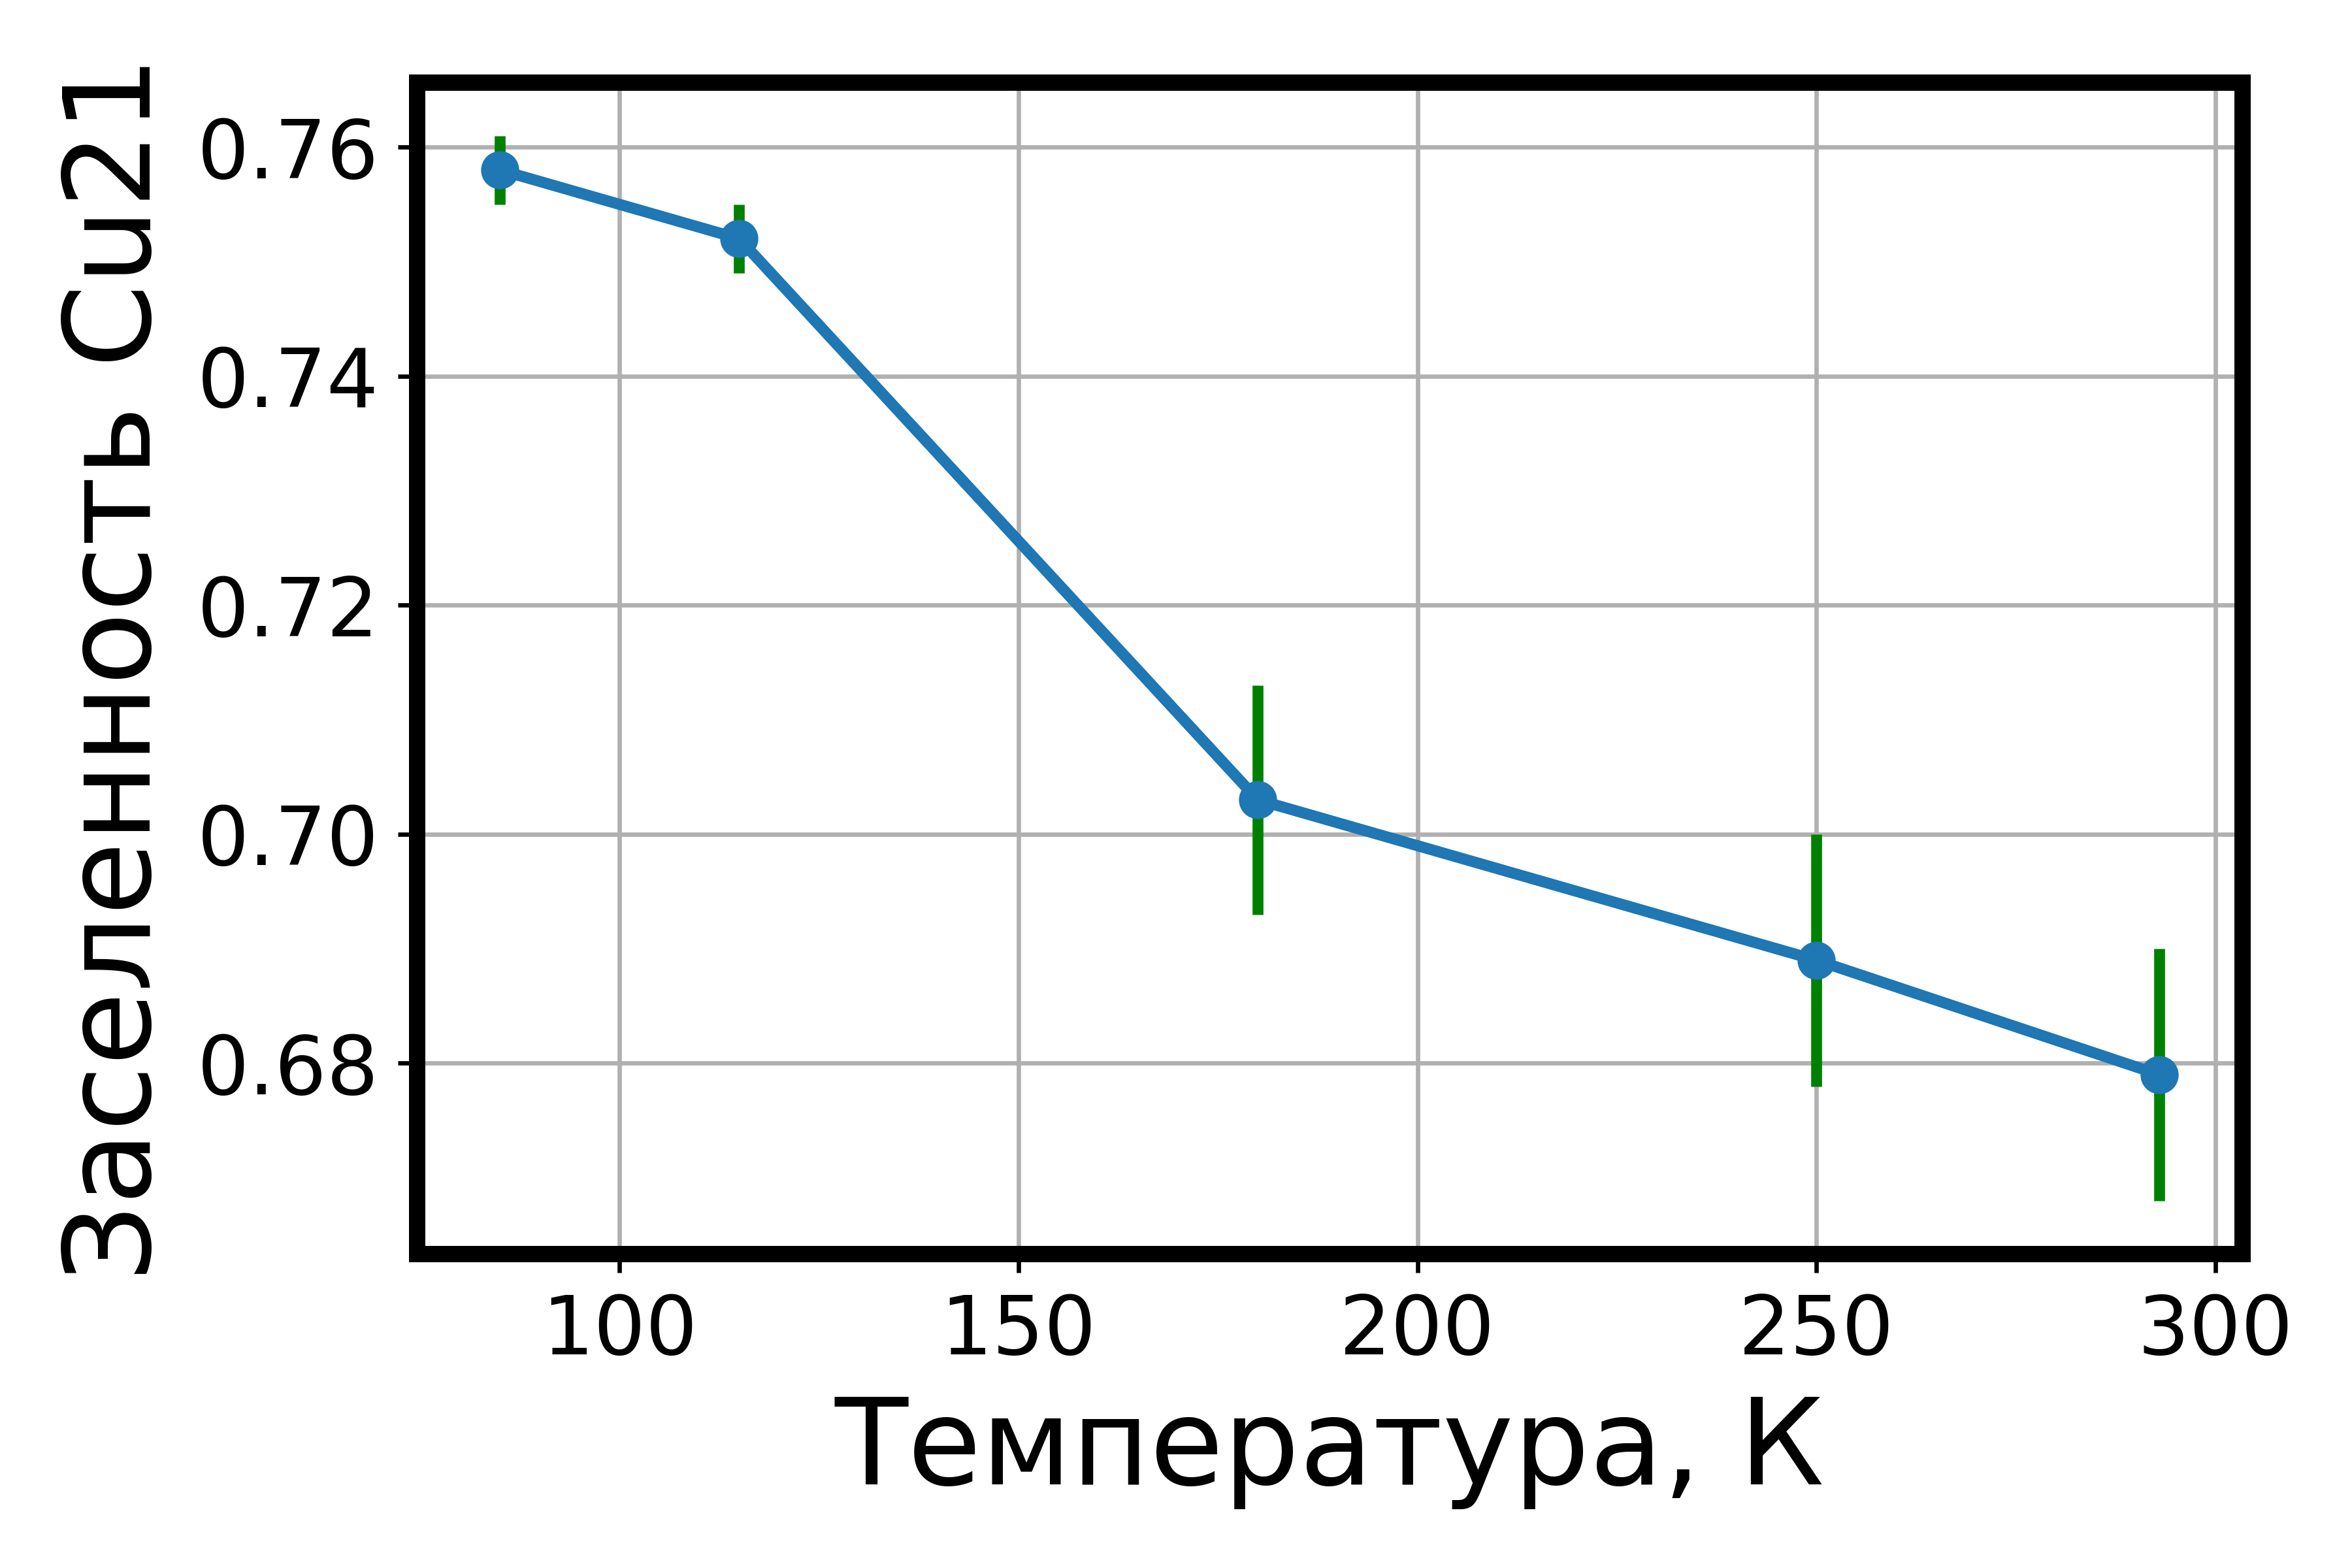
\includegraphics[width=0.9\linewidth]{structure_occCu2} \\ а)
  \end{minipage}
  \vfill
  \begin{minipage}[ht]{0.9\linewidth}\centering
    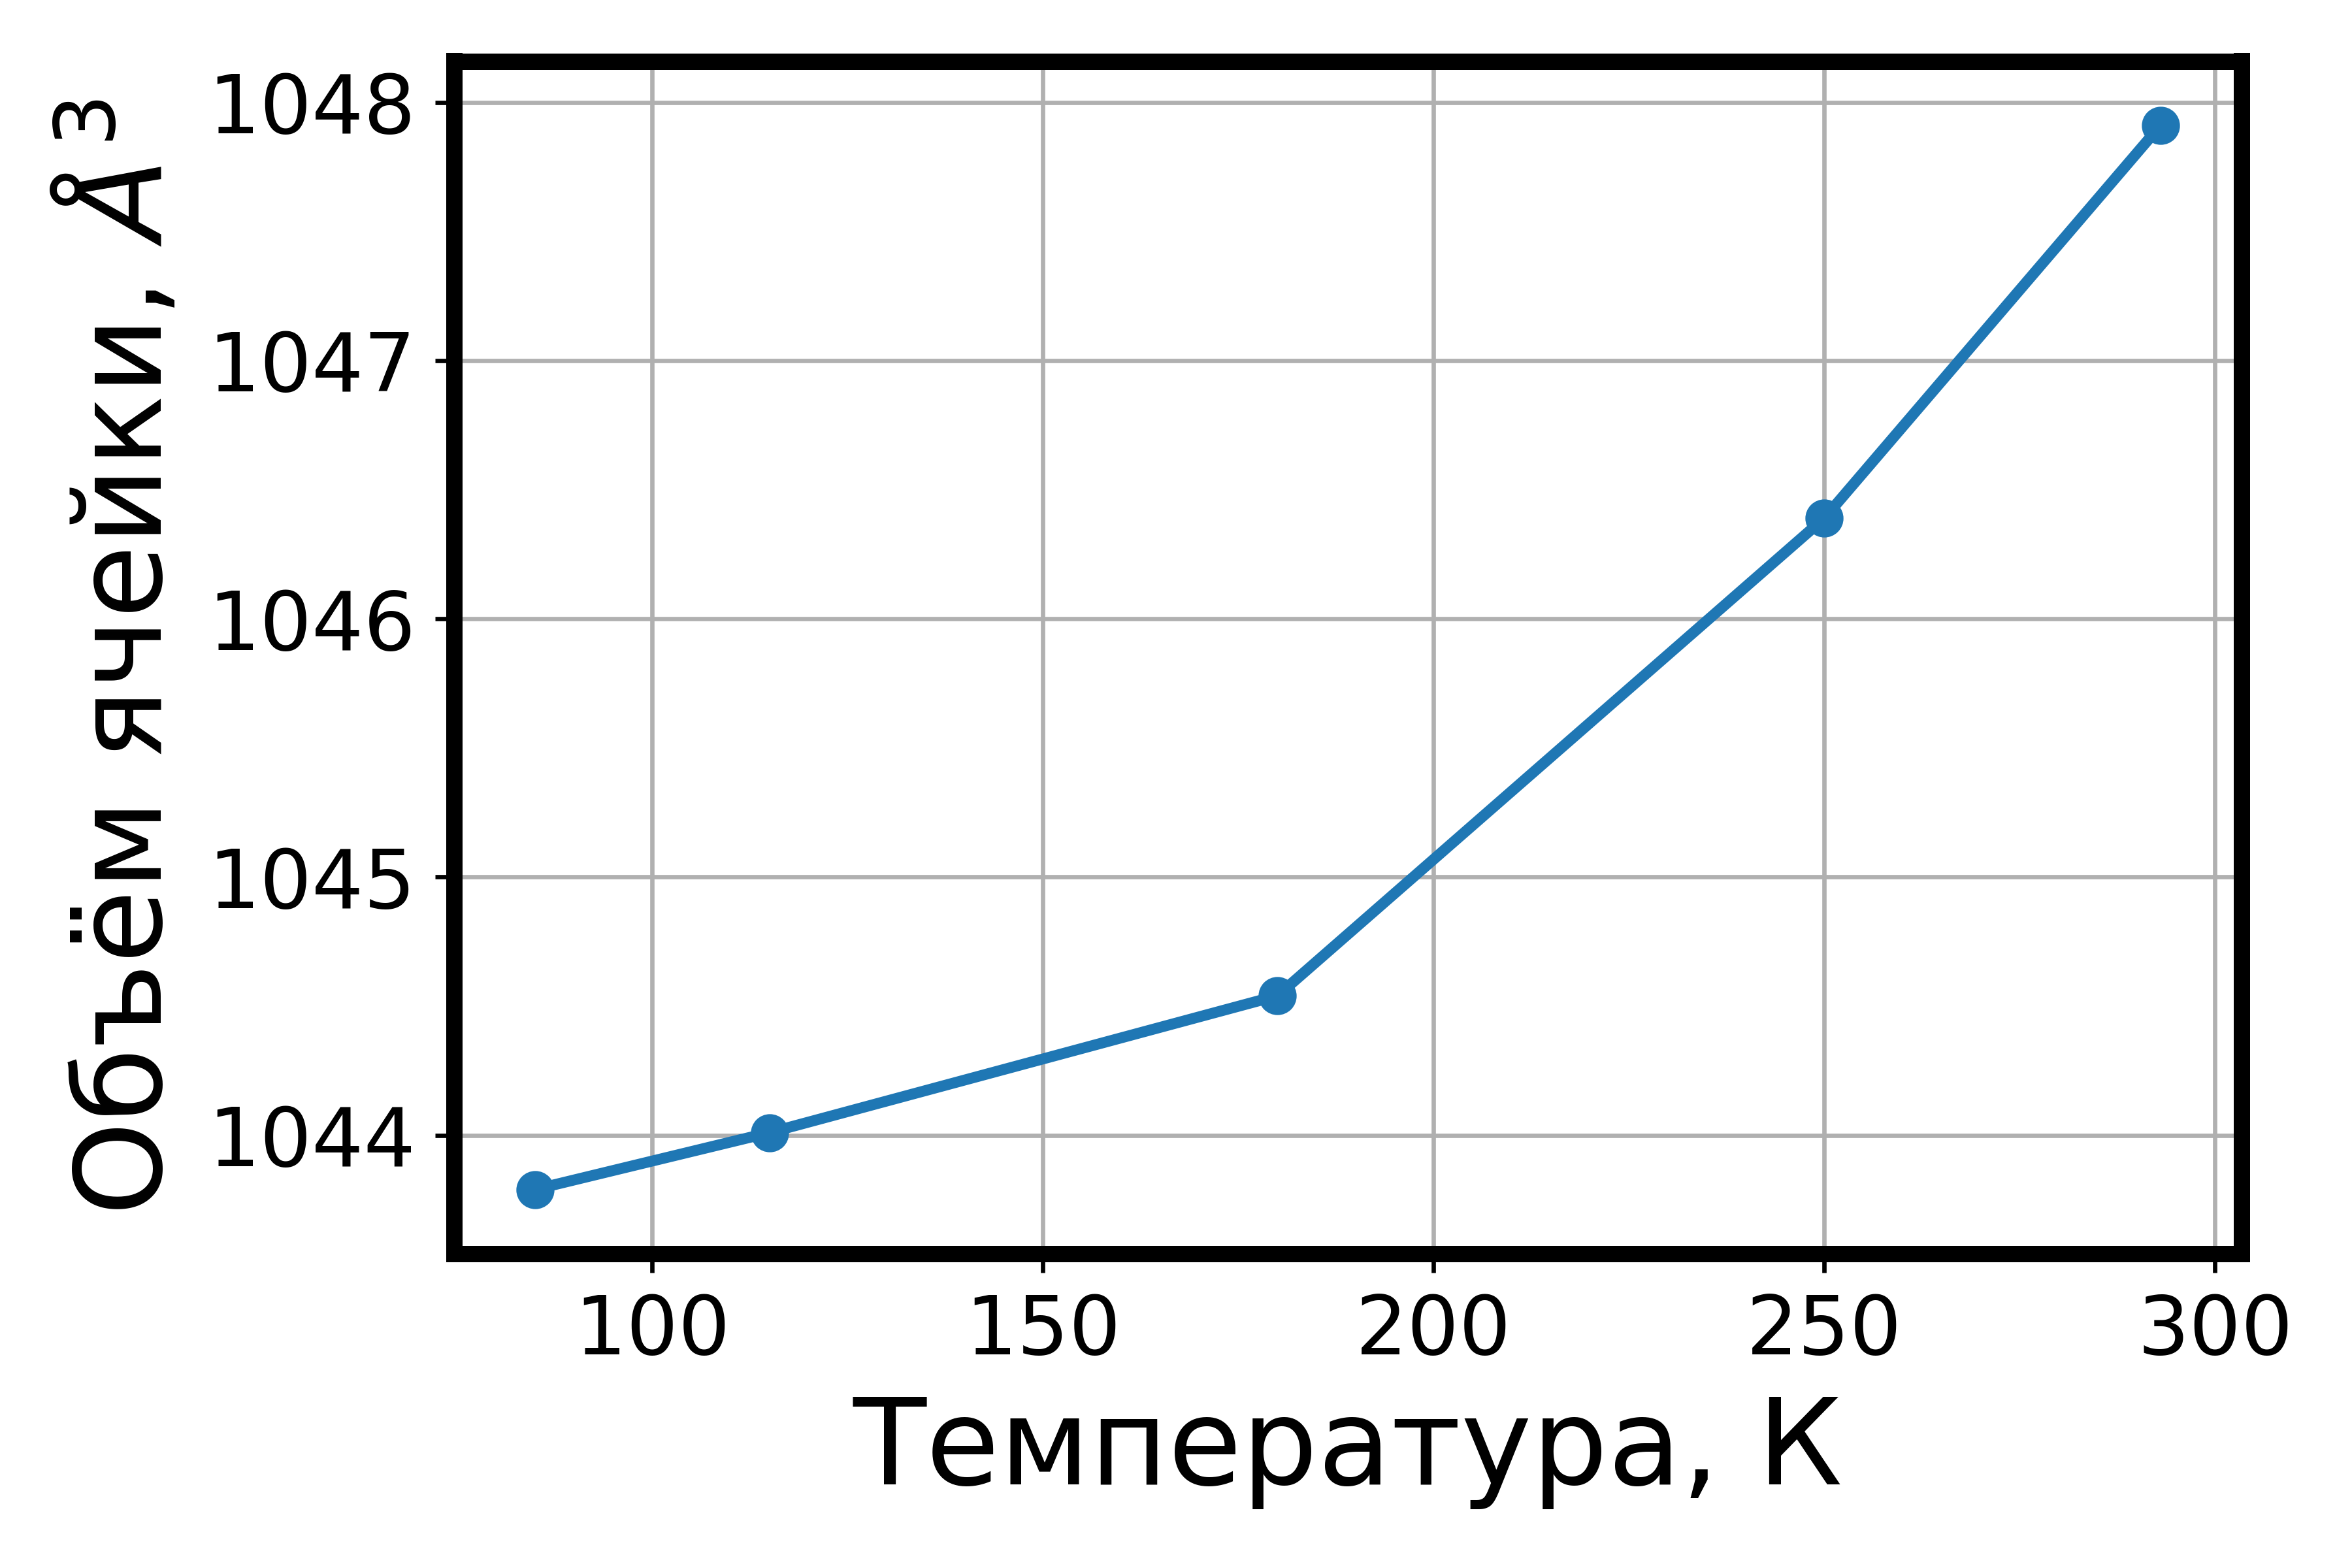
\includegraphics[width=0.9\linewidth]{structure_volume} \\ б)
  \end{minipage}

      \caption[Графики зависимости изменения заселенности для позиции Cu21(а) и объёма кристаллической решетки (б) образца синтетического теннантита Cu\textsubscript{12}As\textsubscript{4}S\textsubscript{13} при температурах 85, 115, 180, 250 и 293~К]{Графики зависимости изменения заселенности для позиции Cu21 (а) и объёма кристаллической решетки(б) образца синтетического теннантита Cu\textsubscript{12}As\textsubscript{4}S\textsubscript{13} при температурах 85, 115, 180, 250 и 293~К}
    \label{img:structure1}
\end{figure}

\begin{figure}[p!]
  \begin{minipage}[ht]{0.9\linewidth}\centering
    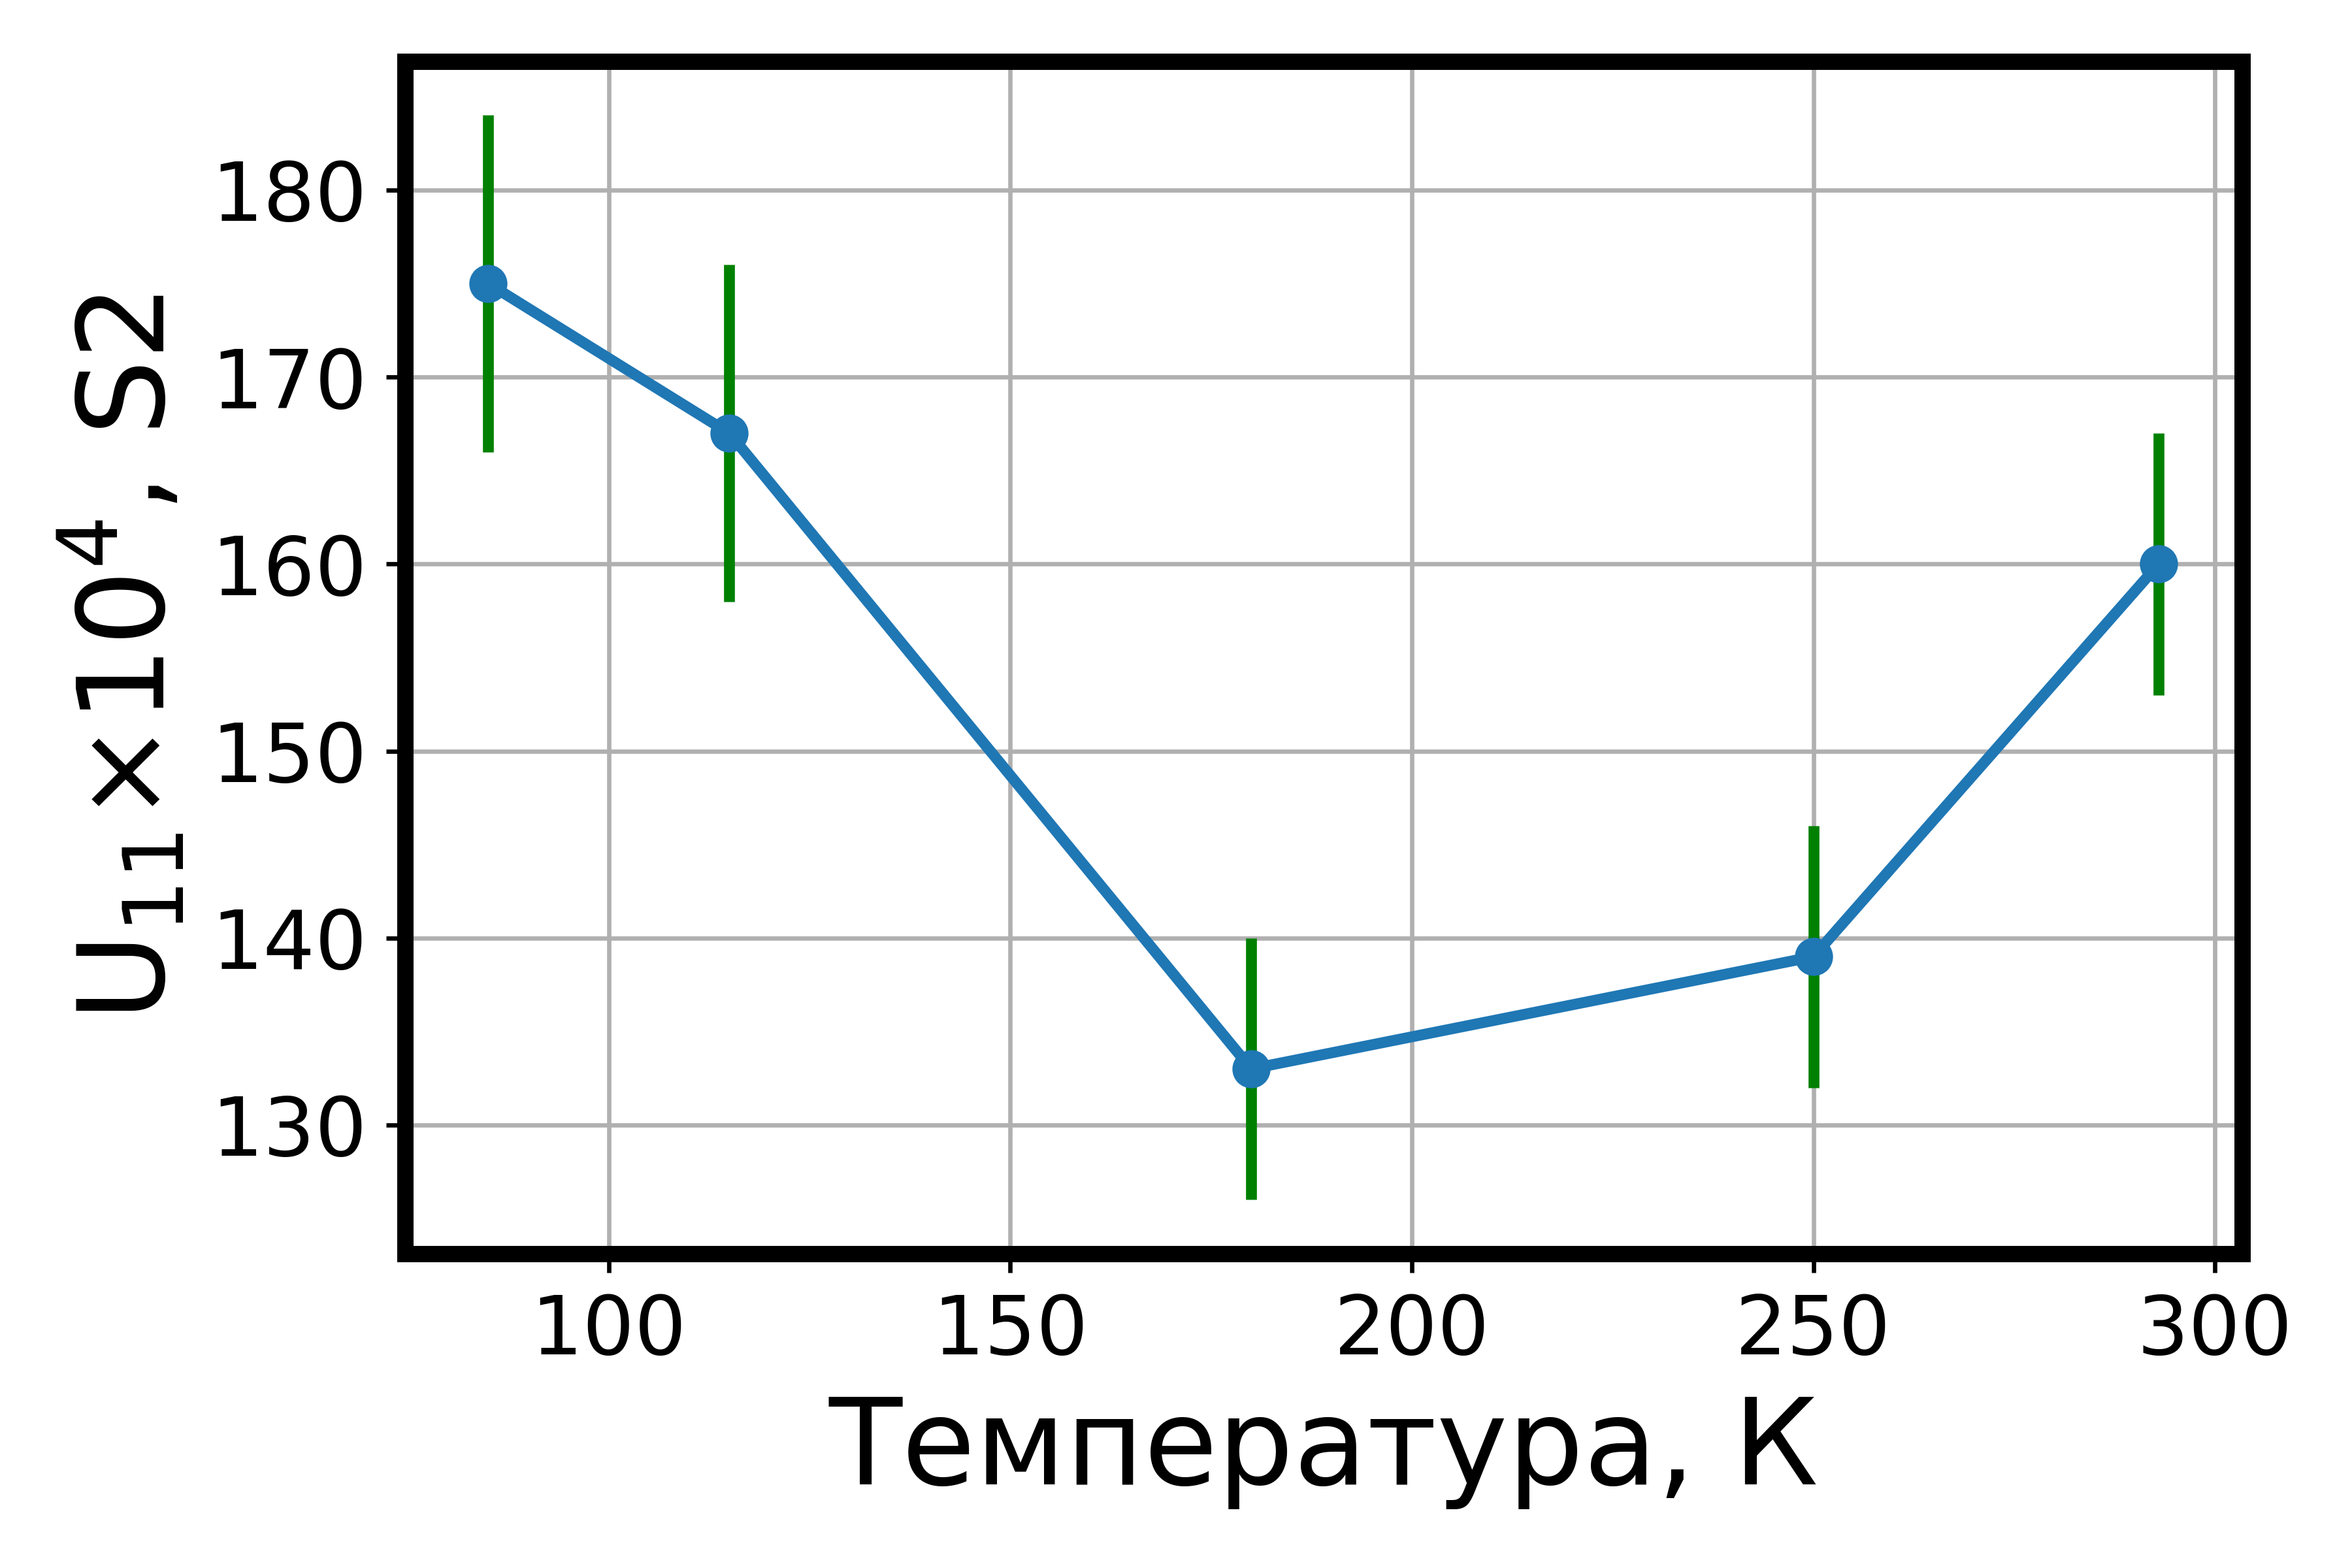
\includegraphics[width=0.9\linewidth]{structure_Ueq} \\ а)
  \end{minipage}
  \vfill
  \begin{minipage}[ht]{0.9\linewidth}\centering
    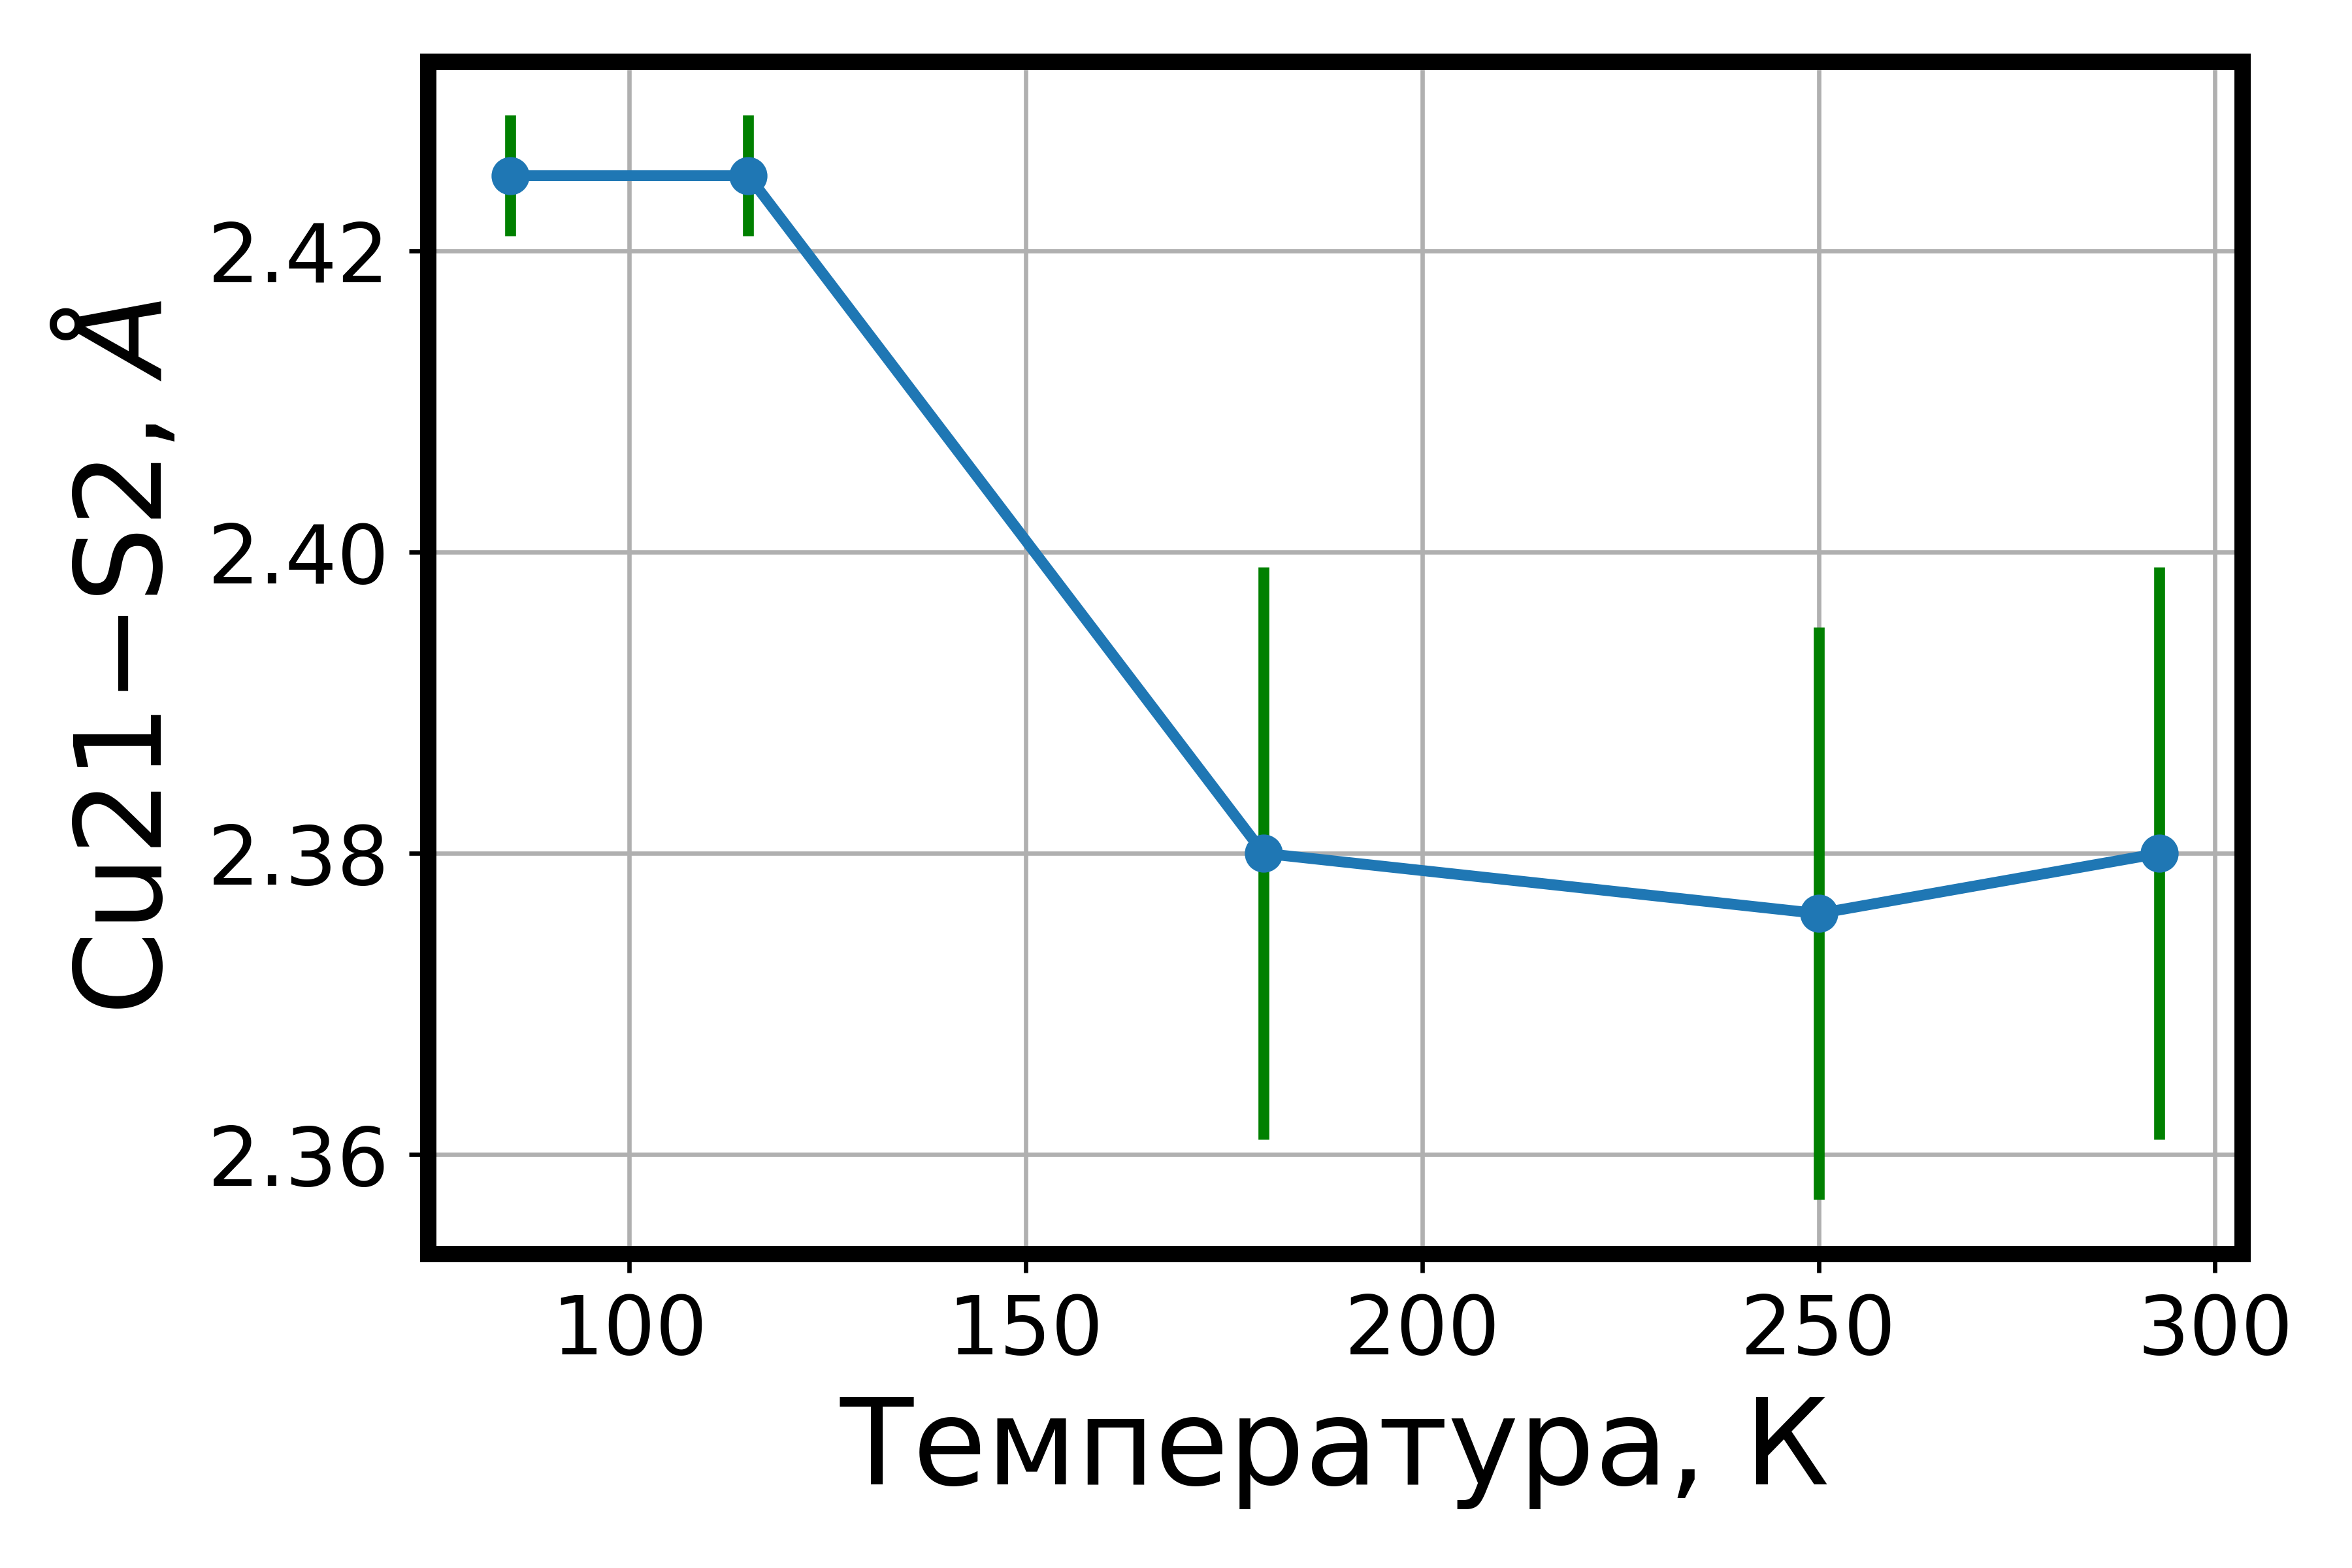
\includegraphics[width=0.9\linewidth]{structure_cu21_s2} \\ б)
  \end{minipage}

      \caption[Графики зависимости атомарного смещения U\textsubscript{11} (а) и расстояния между позициями Cu21--S2 (б) для образца синтетического теннантита Cu\textsubscript{12}As\textsubscript{4}S\textsubscript{13} при температурах 85, 115, 180, 250 и 293~К]{Графики зависимости атомарного смещения U\textsubscript{11} (а) и расстояния между позициями Cu21--S2 (б) для образца синтетического теннантита Cu\textsubscript{12}As\textsubscript{4}S\textsubscript{13} при температурах 85, 115, 180, 250 и 293~К}
    \label{img:structure2}
\end{figure}
\newpage

\section{Электронная просвечивающая микроскопия монокристаллического образца синтетического теннантита Cu\textsubscript{12}As\textsubscript{4}S\textsubscript{13} в плоскости (011) } \label{sect3_2}

Исследования особенностей распределения меди в образце проведены при комнатной температуре на ламельке толщиной менее 100~нм для кристаллографической плоскости (011).
Установлено, что в образце синтетического теннантита Cu\textsubscript{12}As\textsubscript{4}S\textsubscript{13} есть различия значения эллиптичности в рядах меди Cu (Рис. \ref{img:mic}).

\begin{figure}[h!]
  \begin{minipage}[ht]{0.9\linewidth}\centering
    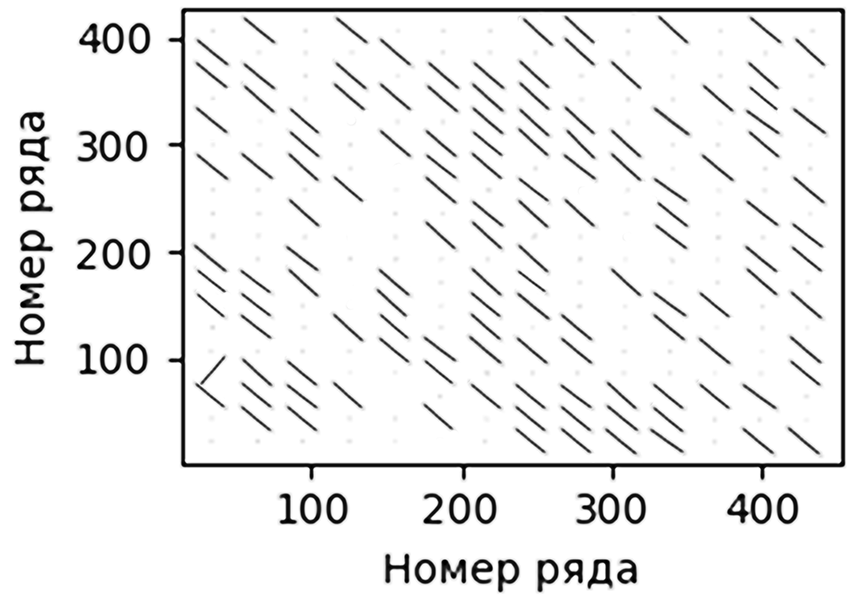
\includegraphics[width=0.7\linewidth]{mic_cupper_raw}
  \end{minipage}

      \caption[Величина и разворот эллиптичности рядов Cu в кристаллографической плоскости (011) синтетического теннантита Cu\textsubscript{12}As\textsubscript{4}S\textsubscript{13}]{Величина и разворот эллиптичности рядов Cu в кристаллографической плоскости (011) синтетического теннантита Cu\textsubscript{12}As\textsubscript{4}S\textsubscript{13}}
    \label{img:mic}
\end{figure}


На рисунке \ref{img:mic2} электронная дифракция для плоскости (011) ламельки синтетического образца Cu\textsubscript{12}As\textsubscript{4}S\textsubscript{13}.
Дифракция обладает отлично определяемыми пиками, которые хорошо идентифицируются (рис. \ref{img:mic2}(б)).

\begin{figure}[ph!]
\centering
  \begin{minipage}[ht]{0.7\linewidth}\centering
    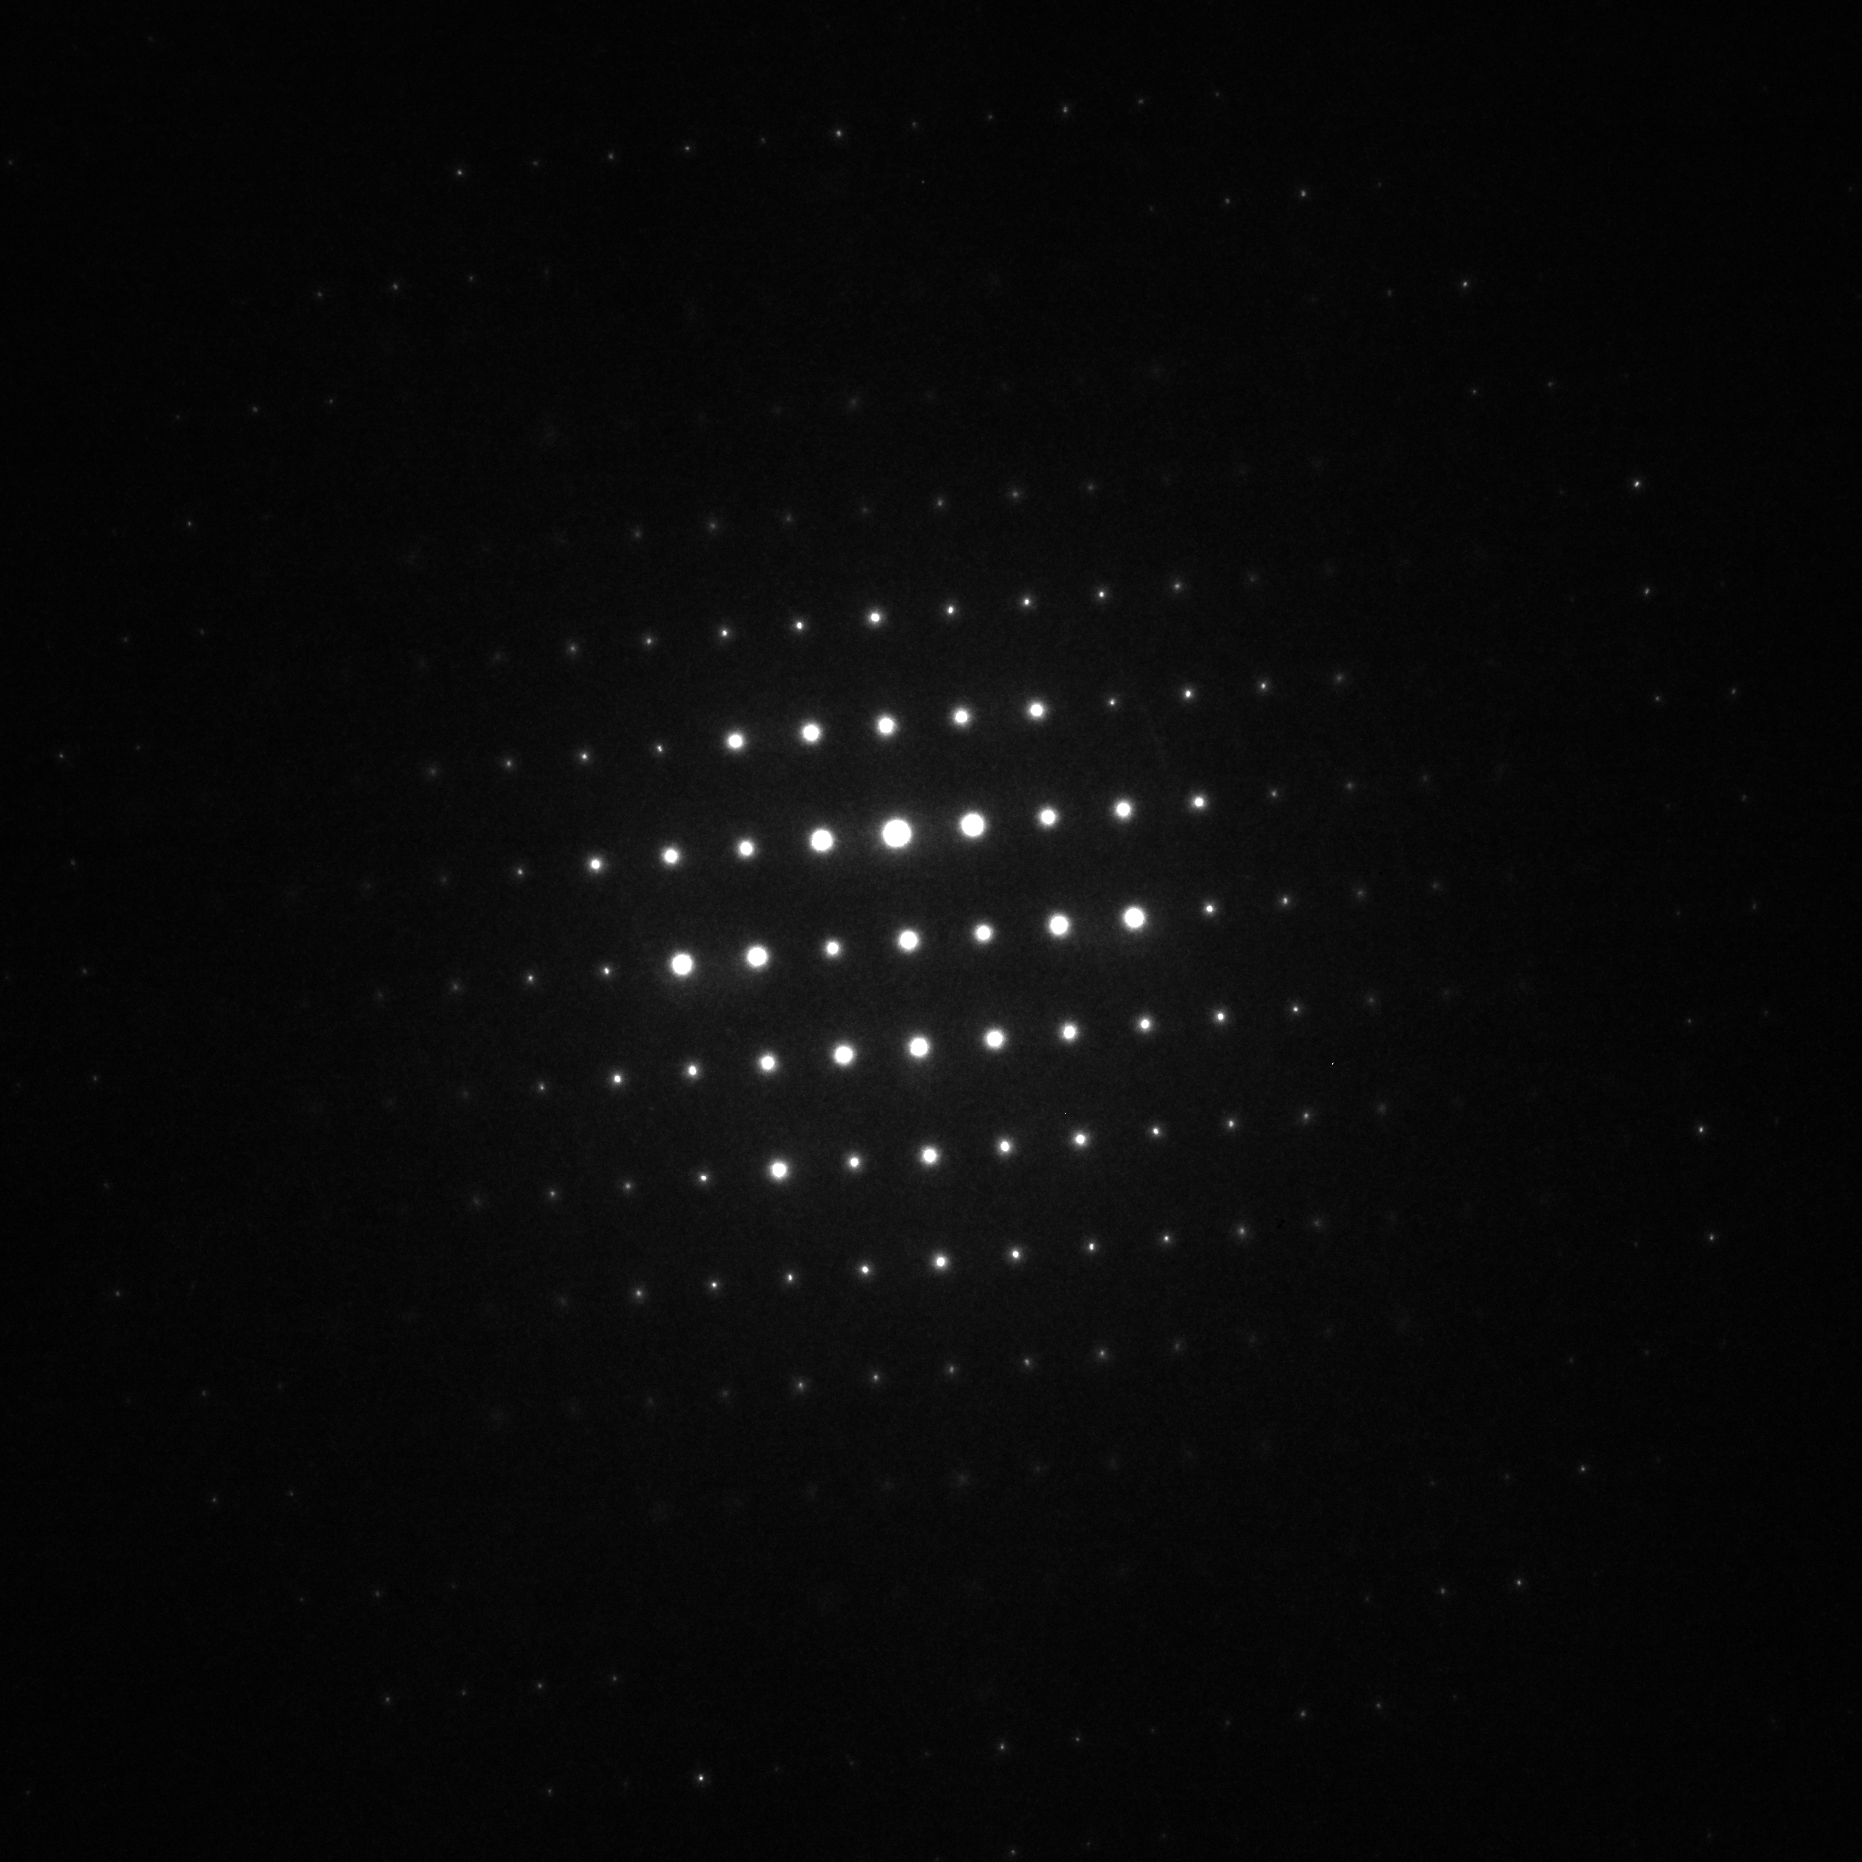
\includegraphics[width=0.9\linewidth]{difr01_el_mic} \\ а)
  \end{minipage}
  \vfill
  \begin{minipage}[ht]{0.7\linewidth}\centering
    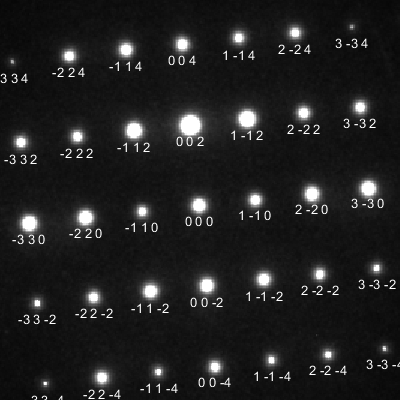
\includegraphics[width=0.9\linewidth]{difr01_el_mic_zone_110} \\ б)
  \end{minipage}
  \caption[Электронная дифракция для плоскости (011) для образца Cu\textsubscript{12}As\textsubscript{4}S\textsubscript{13}. Оригинальное изображение (а) и изображение с отмеченными дифракционными рефлексами (б)]{Электронная дифракция для плоскости (011) для образца Cu\textsubscript{12}As\textsubscript{4}S\textsubscript{13}. Оригинальное изображение (а) и изображение с отмеченными дифракционными рефлексами (б)}
    \label{img:mic2}
\end{figure}

Анализ изображения структуры показывает наличие разной эллиптичности для рядов атомов меди. На рисунке \ref{img:mic} представлено наличие эллиптичности атомов рядов меди с учётом дрейфа для плоскости (011) синтетического теннантита Cu\textsubscript{12}As\textsubscript{4}S\textsubscript{13}.




\newpage

\section{Температурная зависимость магнитной восприимчивости многокомпонентных соединений меди} \label{sect3_3}

Полученные графики зависимости магнитной восприимчивости (рис. \ref{img:magsus1} и \ref{img:magsus2}) обладают видом характерным для парамагнетиков с областями отклонения от парамагнитного хода.  Температурные зависимости магнитной восприимчивости для каждого образца были получены в магнитных полях 1, 10, 35 и 70~кЭ. При любом значении магнитного поля графики зависимости магнитной восприимчивости обладают теми же самыми характерными особенностями для каждого образца. Для части образцов были измерены петли гистерезиса, которые показали незначительное наличие ферромагнитных примесей. Также зависимости магнитной восприимчивости для монокристаллического и поликристаллических образцов соединения Cu\textsubscript{12}As\textsubscript{4}Se\textsubscript{13} не отличаются. Все зависимости магнитной восприимчивости приведены с вычетом диамагнитного вклада.

График зависимости для монокристаллического образца Cu\textsubscript{12}As\textsubscript{4}Se\textsubscript{13} в диапазоне температур от 2 до 200 К имеет вид отличный от кривой Кюри"--~Вейса.
 Характер кривой измеренной магнитной восприимчивости образца  Cu\textsubscript{12}As\textsubscript{4}S\textsubscript{13}, показывает наличие возможного перехода из парамагнитного состояния в антиферромагнитное в диапазоне температур от 120 до 130~К (\ref{img:magsus1}а).
До температуры 170 К зависимость парамагнитного вклада магнитной восприимчивости монотонно возрастает с понижением температуры и согласуется с Кюри"--~Вейсовским поведением, характерным для парамагнетика.

\begin{figure}[p!]
  \begin{minipage}[ht]{0.9\linewidth}\centering
    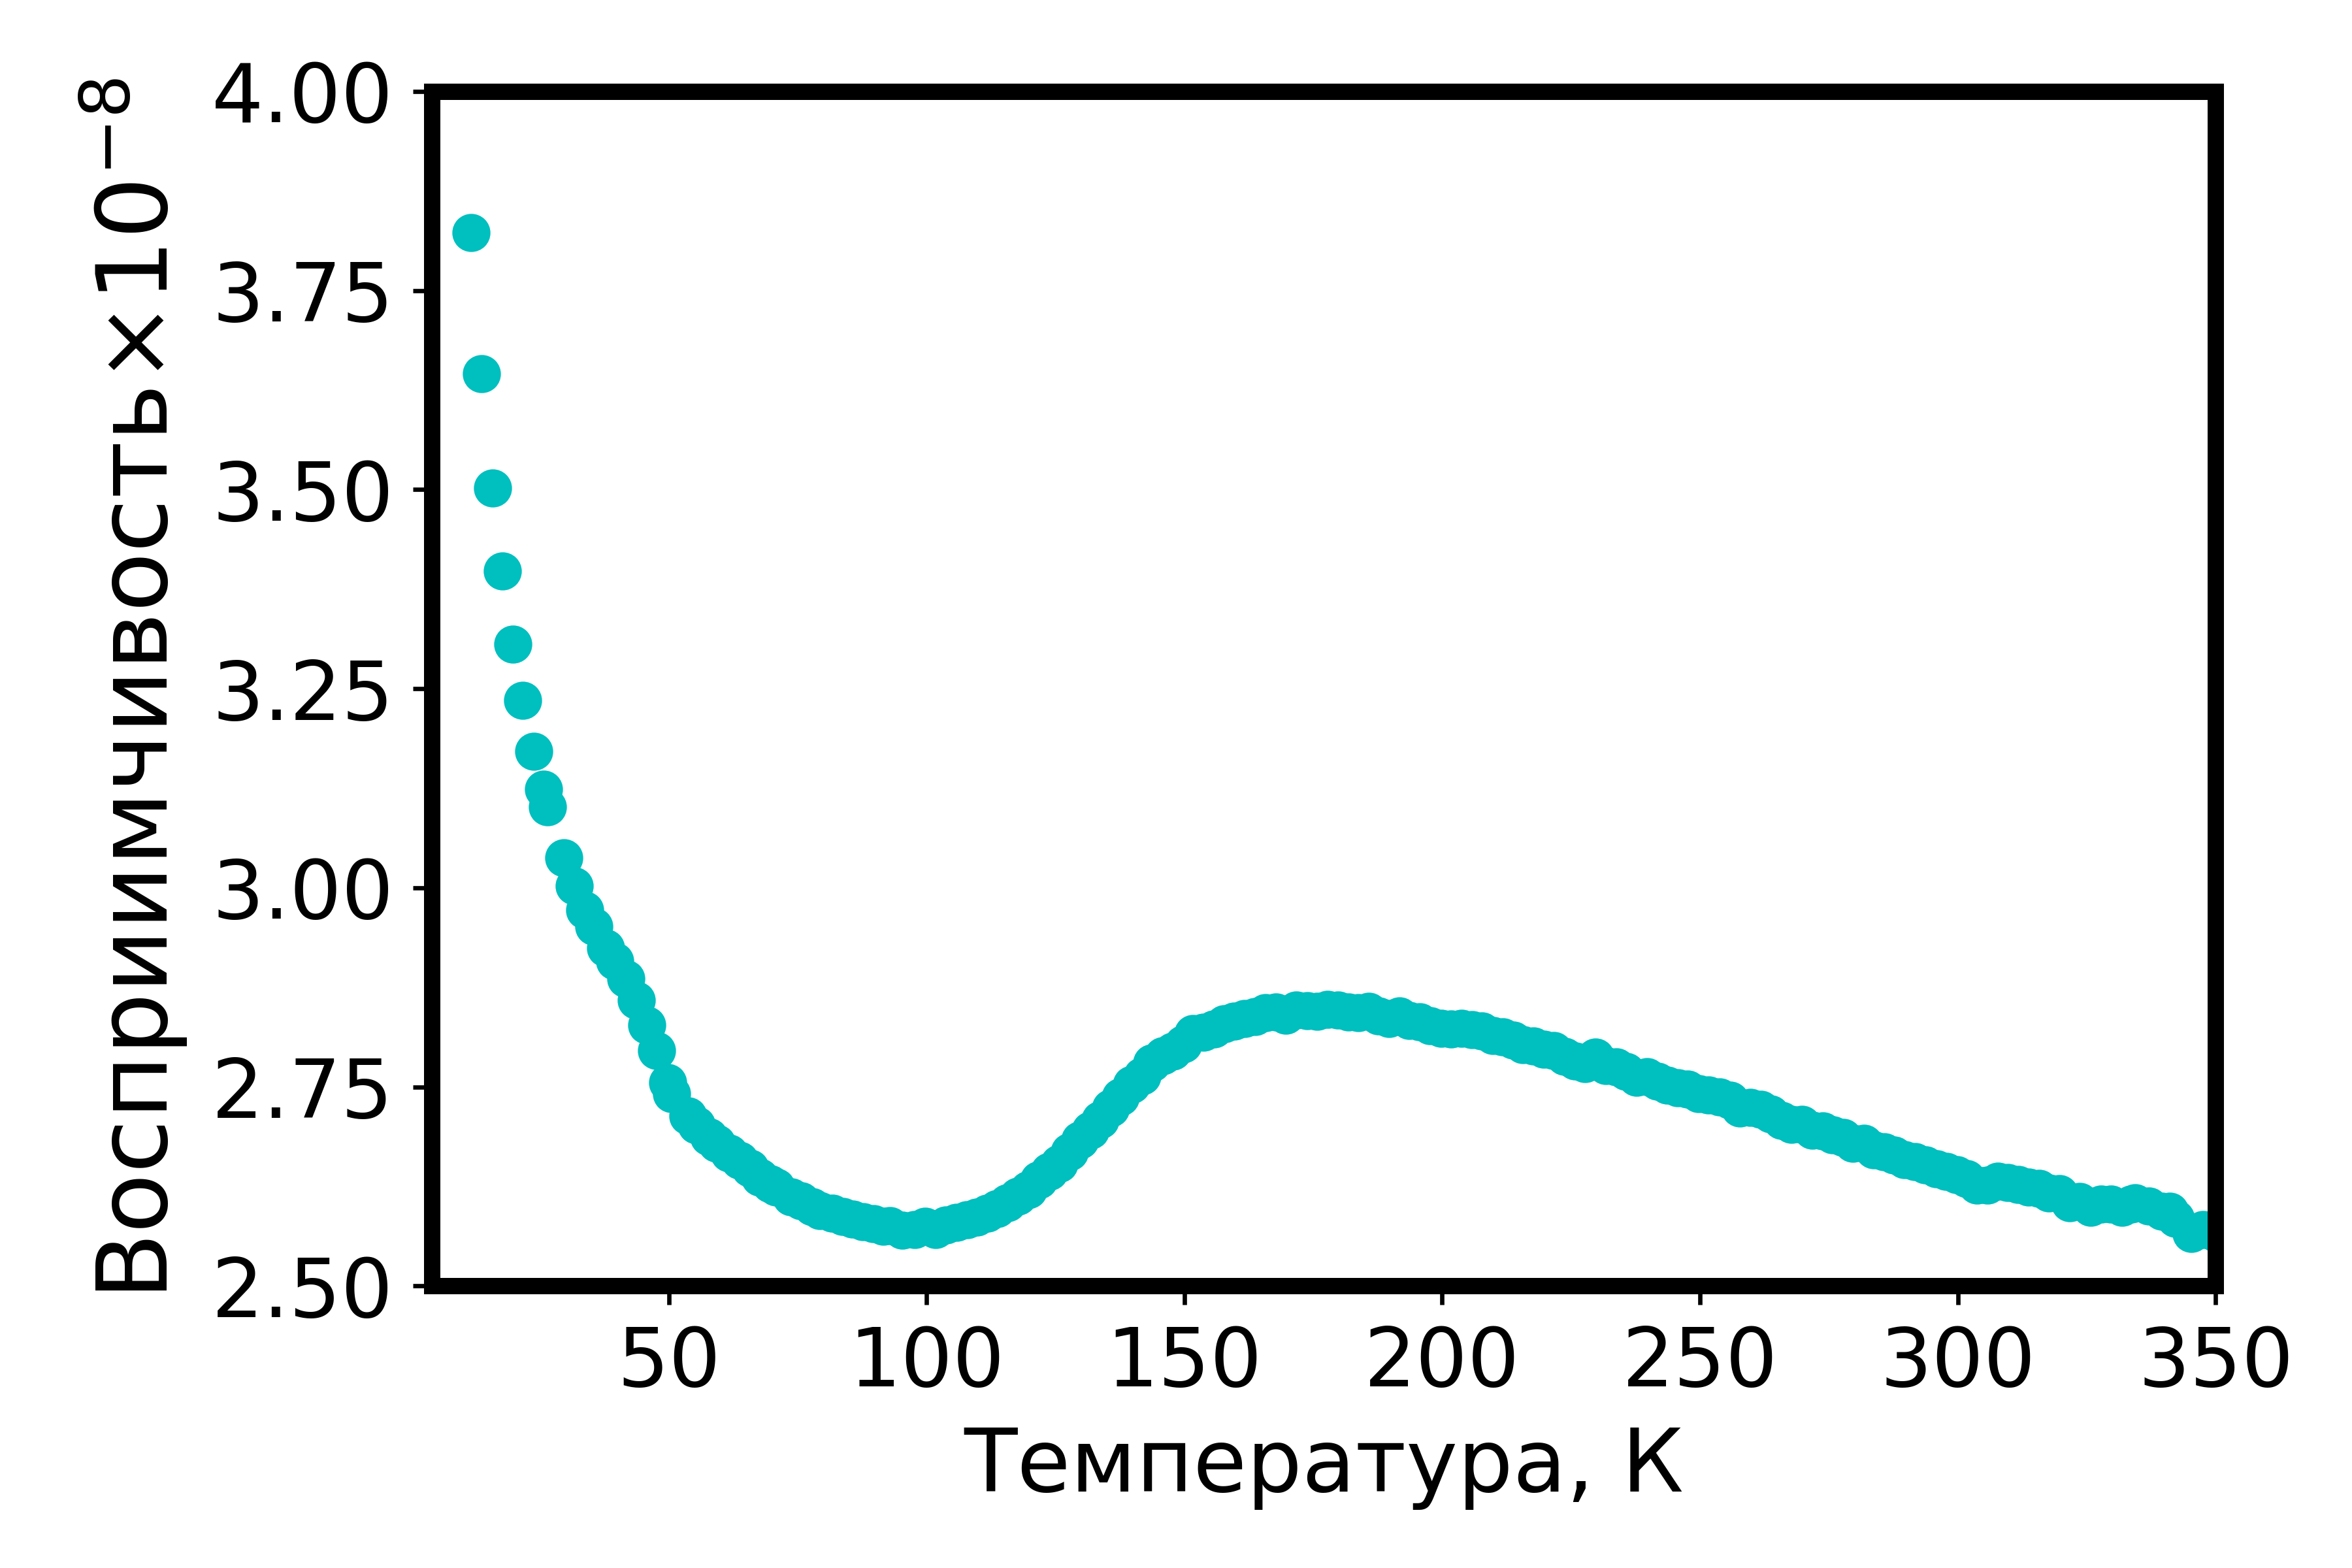
\includegraphics[width=0.9\linewidth]{sus_exp_Cu_As_S} \\ а)
  \end{minipage}
 \vfill
  \begin{minipage}[ht]{0.9\linewidth}\centering
    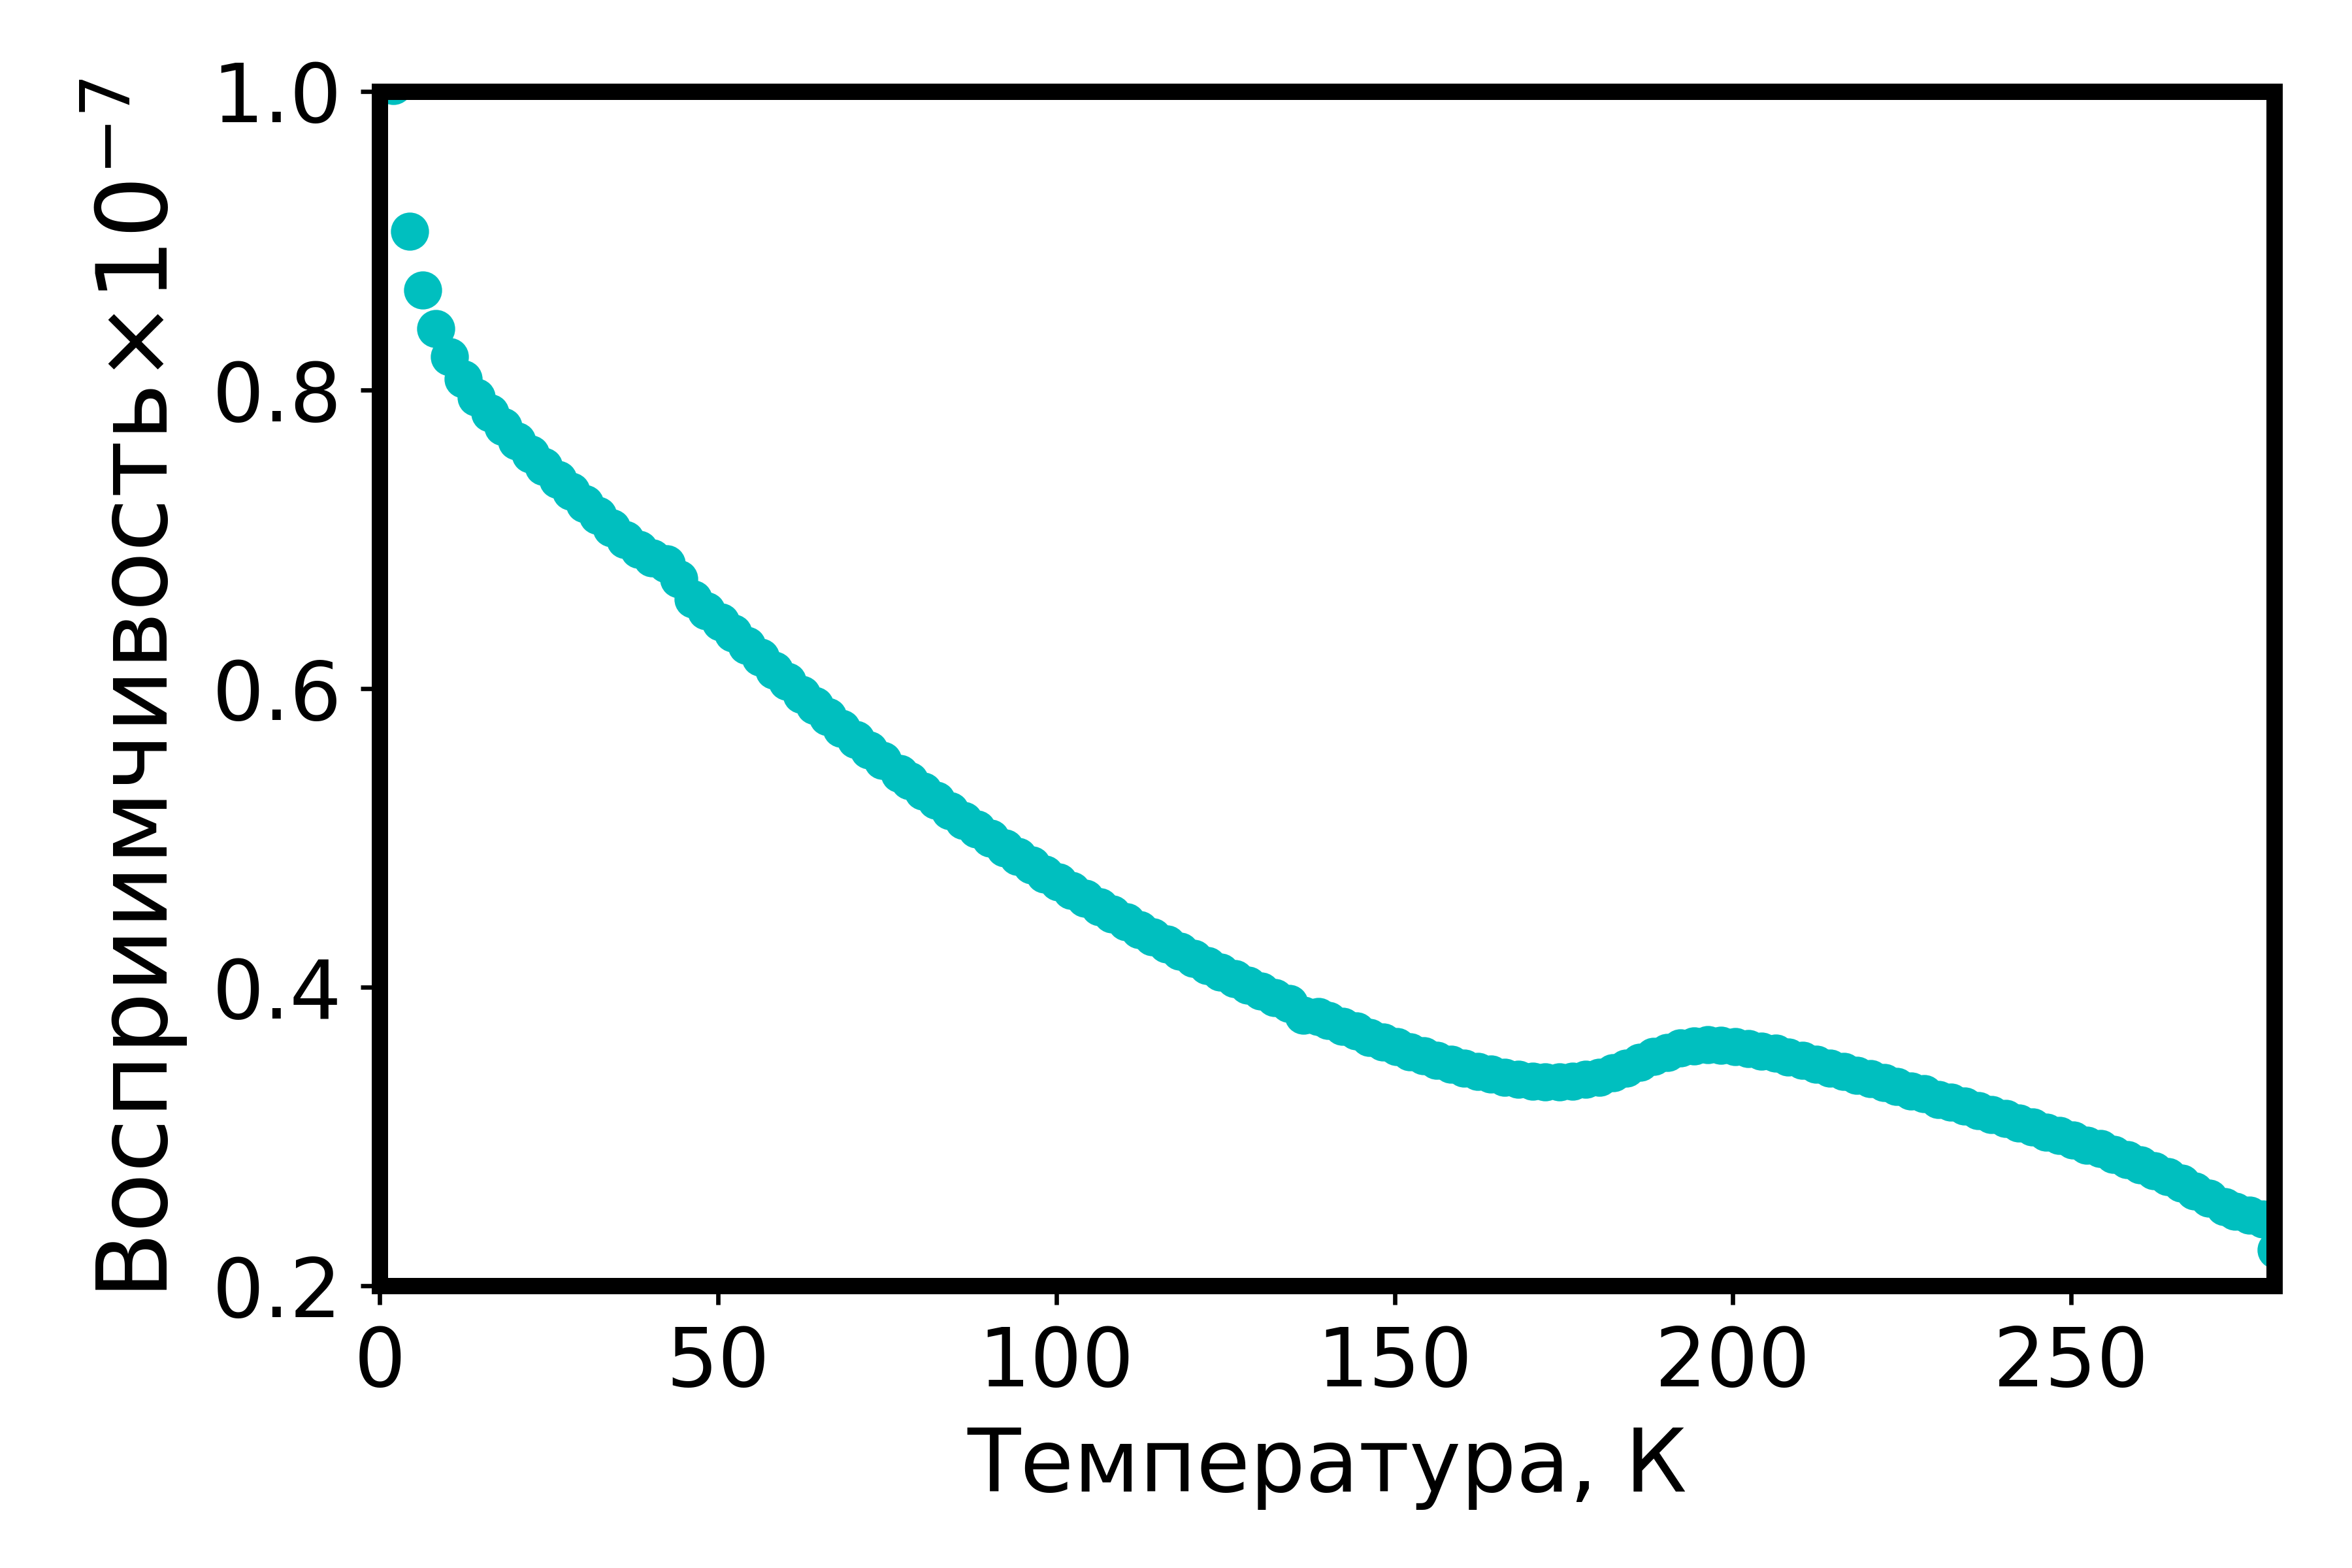
\includegraphics[width=0.9\linewidth]{sus_exp_Cu_As_Se} \\ б)
  \end{minipage}
      \caption[Графики зависимости магнитно	й восприимчивости для образцов Cu\textsubscript{12}As\textsubscript{4}Se\textsubscript{13} (а) и Cu\textsubscript{3}AsS\textsubscript{3} (б)]{Графики зависимости магнитно	й восприимчивости для образцов Cu\textsubscript{12}As\textsubscript{4}S\textsubscript{13} (а) и Cu\textsubscript{3}AsSe\textsubscript{3} (б)}
    \label{img:magsus1}
\end{figure}

График зависимости удельной намагниченности образца Cu\textsubscript{3}AsSe\textsubscript{3} от температуры, измеренный в магнитном поле напряженностью 10 кЭ, представлен на рис. \ref{img:magsus1}б.
При температуре 44 К наблюдается пик магнитной восприимчивости, в интервале температур 170--200 К происходит рост магнитной восприимчивости, а при температуре 285--295 К происходит ее падение.
По-видимому, в интервале температур 170--295 К реализуется особое магнитное состояние в соединении синтетического мгриита.

При температурах 2, 250 и 300~К измерены петли гистерезиса (рис. \ref{img:magsus3}) для образца Cu\textsubscript{3}AsSe\textsubscript{3}.
Рост намагниченности при увеличении температуры при температурах 2 и 250 К также говорит о
том, что исследуемое соединение является парамагнетиком.
Однако, для температур выше 300 К намагниченность становится отрицательной, что
говорит о доминировании диамагнетизма.
 Ветви петли гистерезиса располагаются во втором и четвертом квадрантах, что соответствует диамагнетикам.
Детальное исследование в области малых магнитных полей при учете парамагнетизма (при 2 и 250 К) или диамагнетизма (при 300 К) позволили обнаружить слабый ферромагнетизм в исследуемом соединении, который, по-видимому, связан с наличием ферромагнитных примесей в синтезированном соединении.
Увеличенные петли гистерезиса представлены на вставке рисунка \ref{img:magsus3}.



\begin{figure}[pt!]
  \begin{minipage}[ht]{0.9\linewidth}\centering
    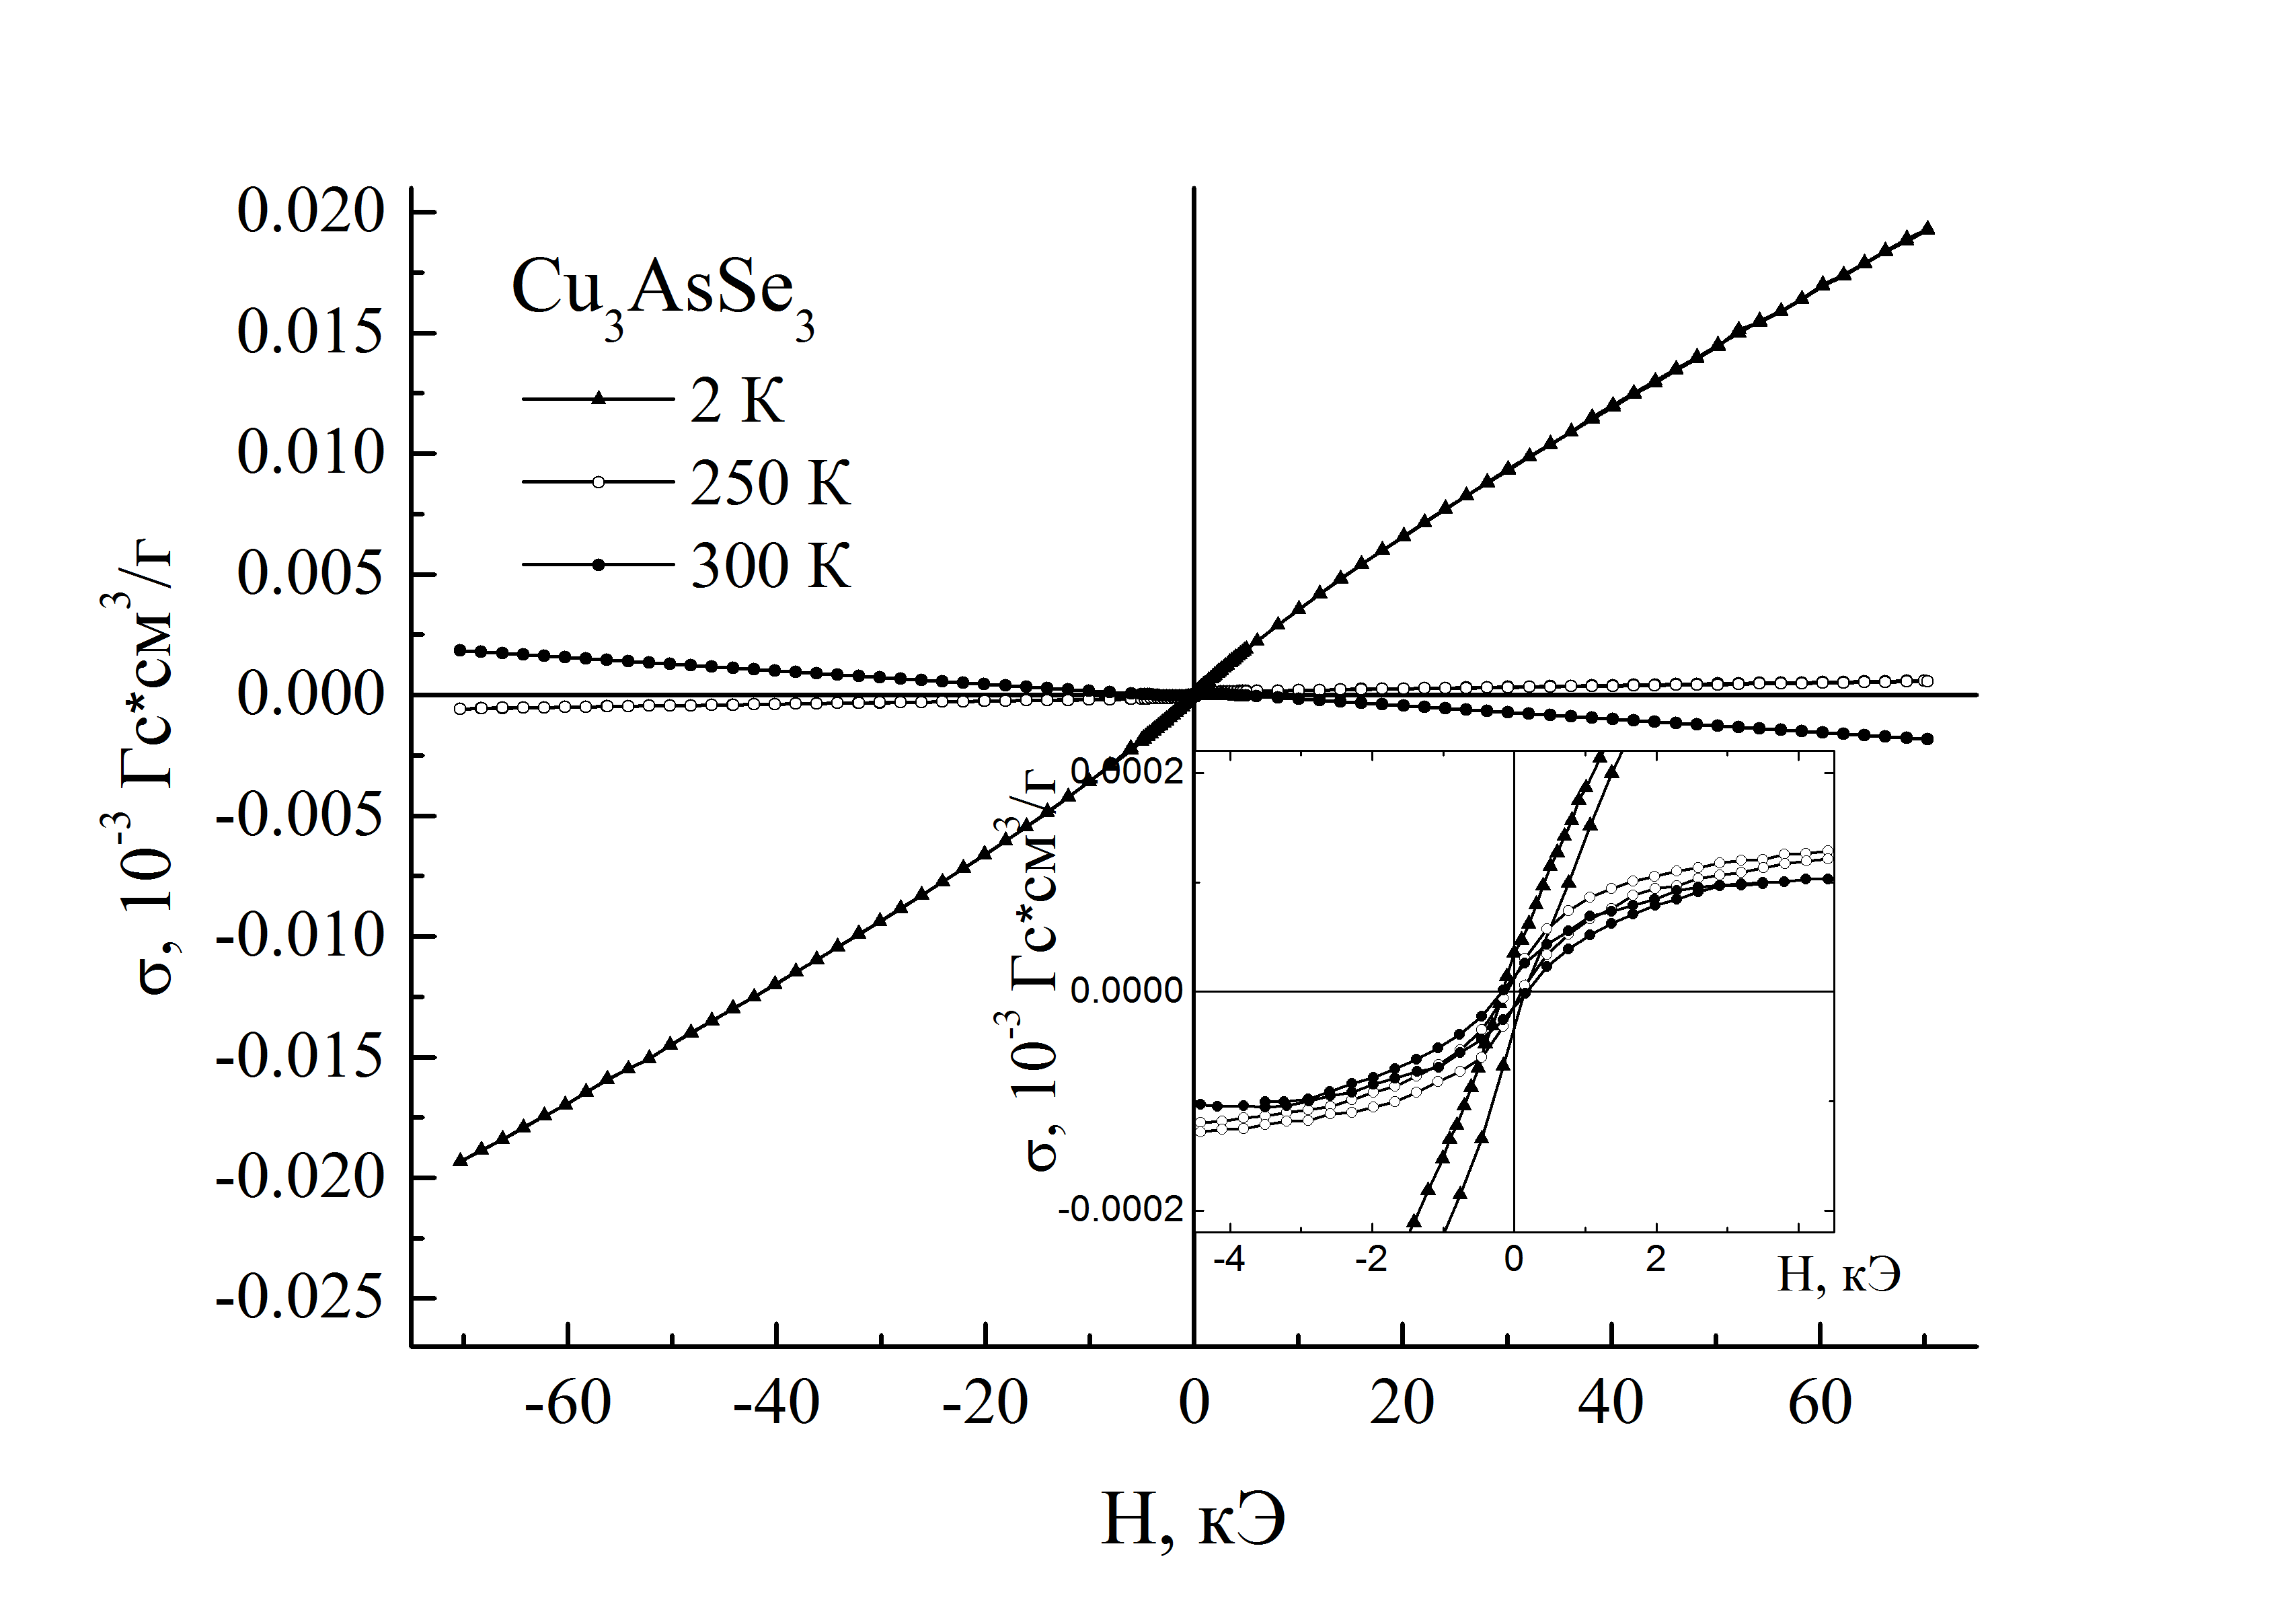
\includegraphics[width=0.9\linewidth]{sigma_mag} \\
  \end{minipage}

      \caption[Графики зависимости удельной намагниченности в магнитных полях от $-$70 до 70~кЭ при температурах 2, 250 и 300~К для образца Cu\textsubscript{3}AsSe\textsubscript{3}]{Графики зависимости удельной намагниченности в магнитных полях от $-$70 до 70~кЭ при температурах 2, 250 и 300~К для образца Cu\textsubscript{3}AsSe\textsubscript{3}}
    \label{img:magsus3}
\end{figure}


\begin{figure}[pt!]
  \begin{minipage}[ht]{0.9\linewidth}\centering
    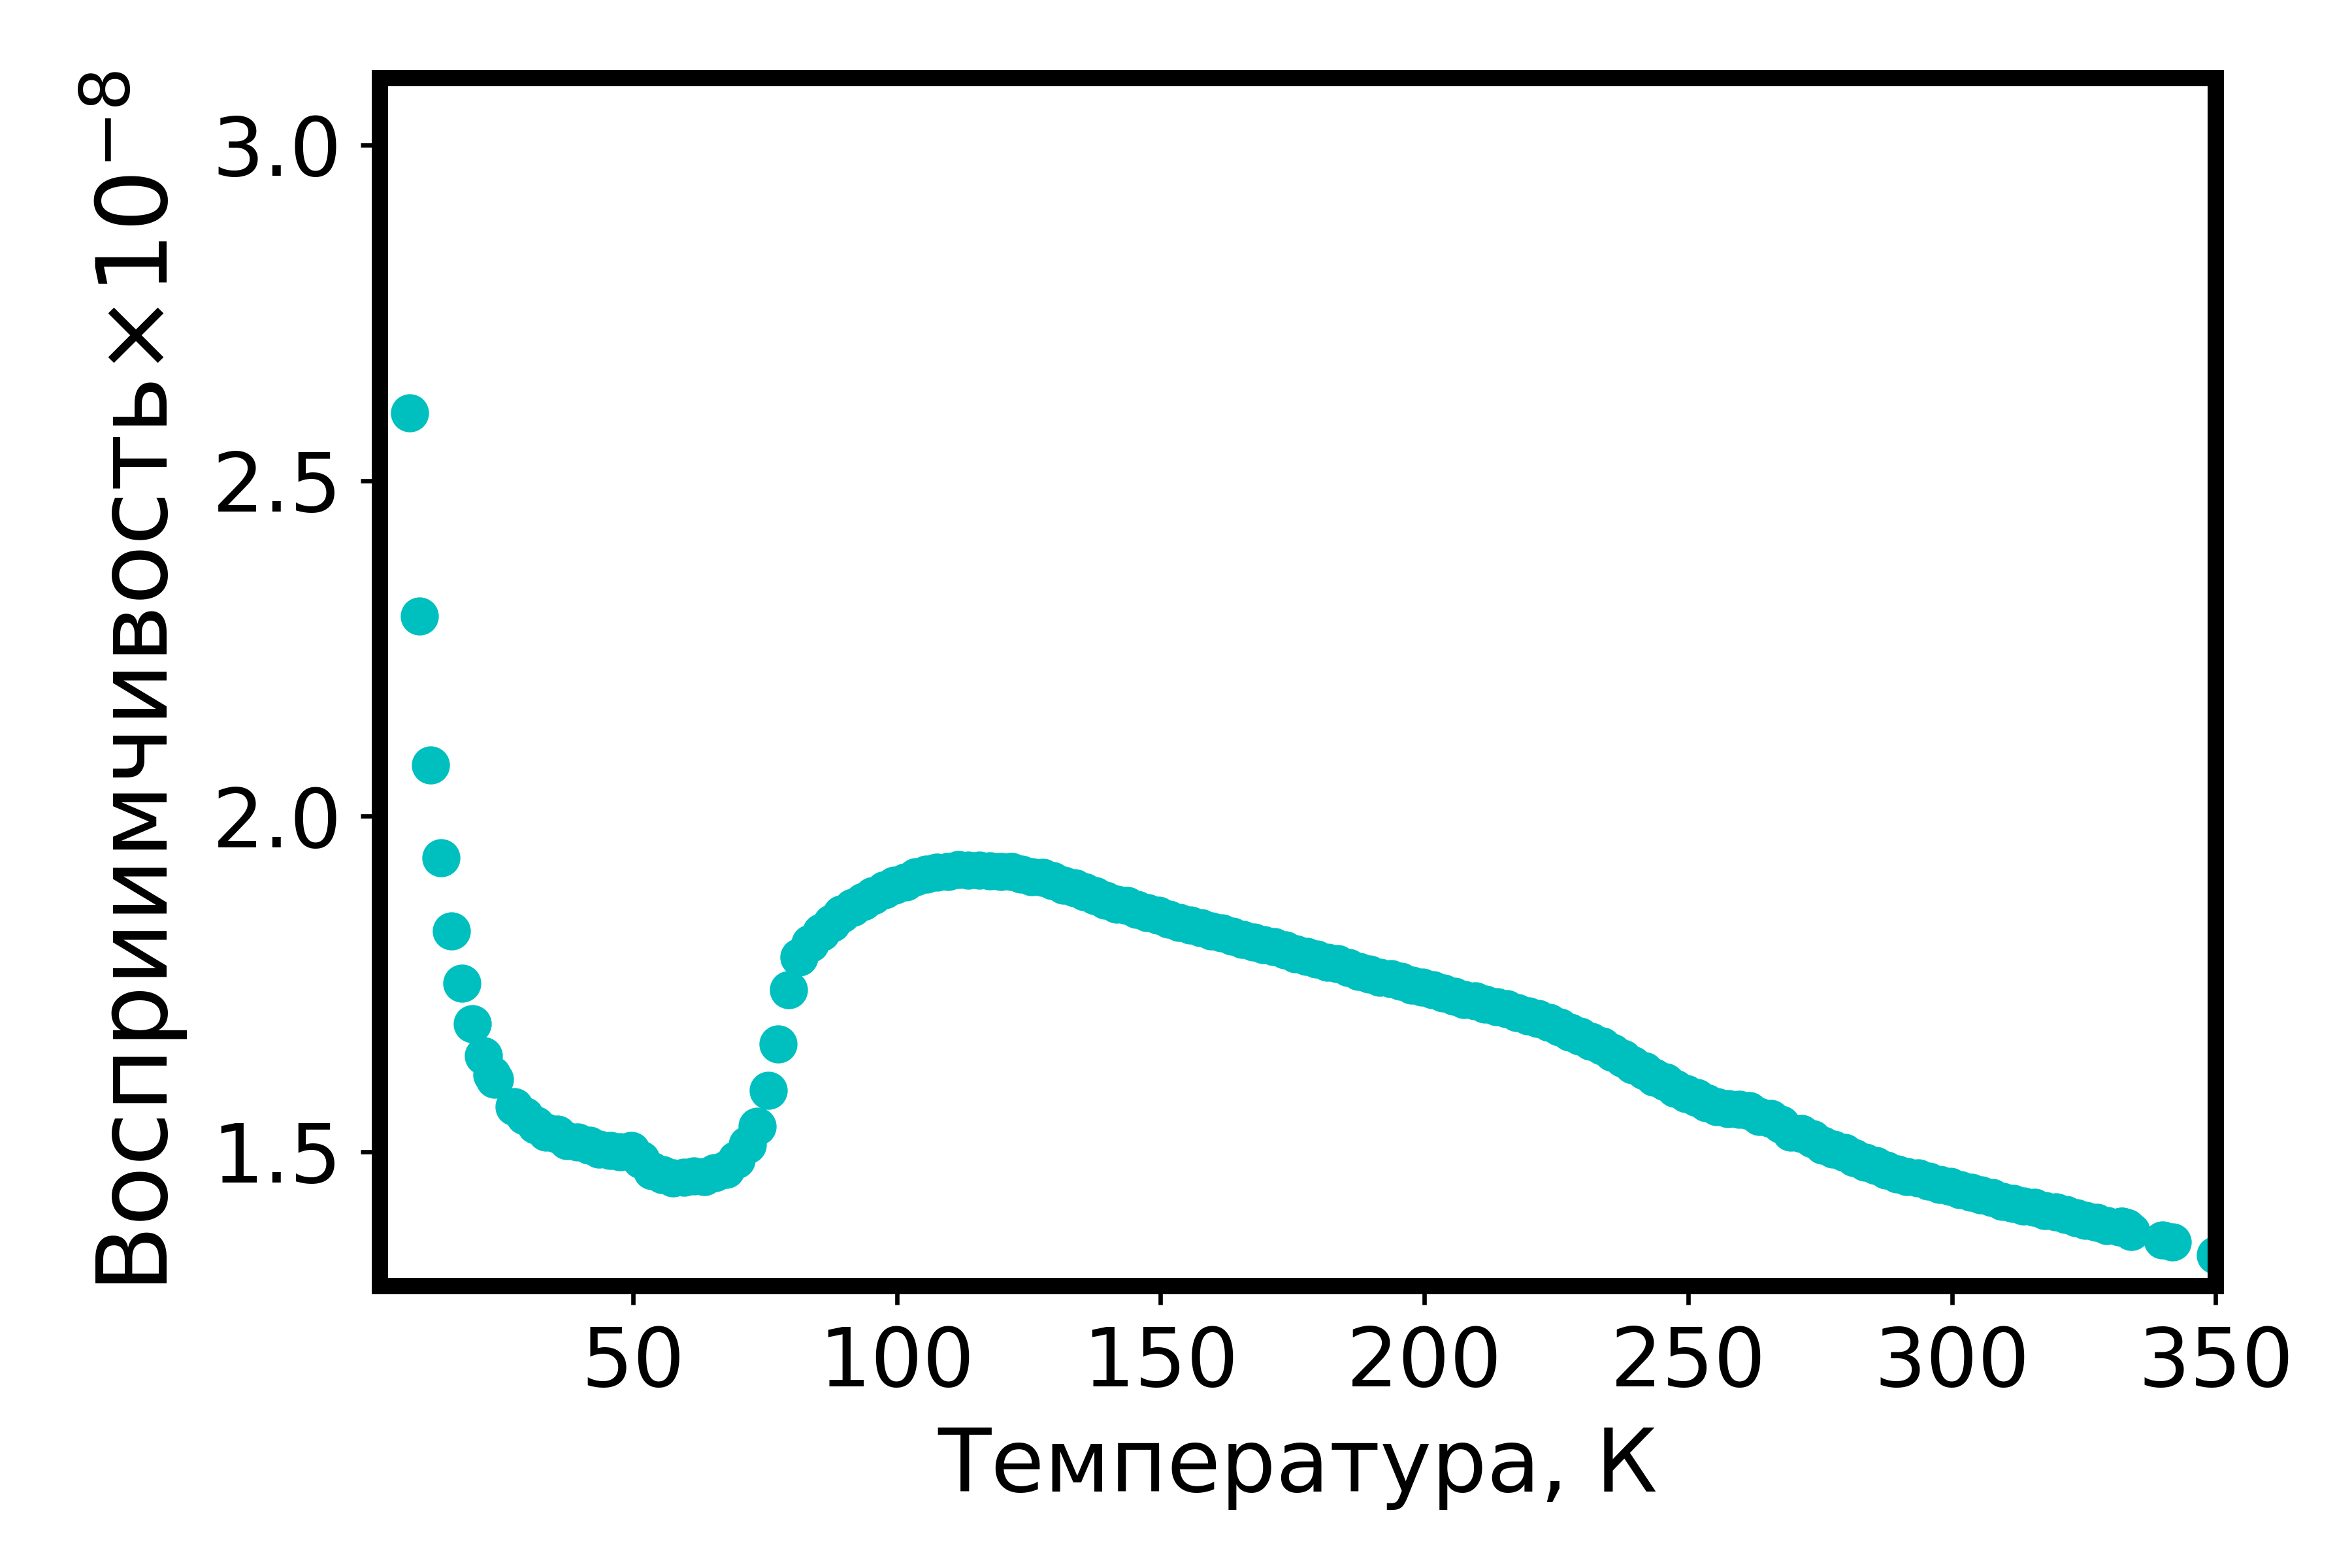
\includegraphics[width=0.9\linewidth]{sus_exp_Cu_Sb_S} \\ а)
  \end{minipage}
\vfill
  \begin{minipage}[ht]{0.9\linewidth}\centering
    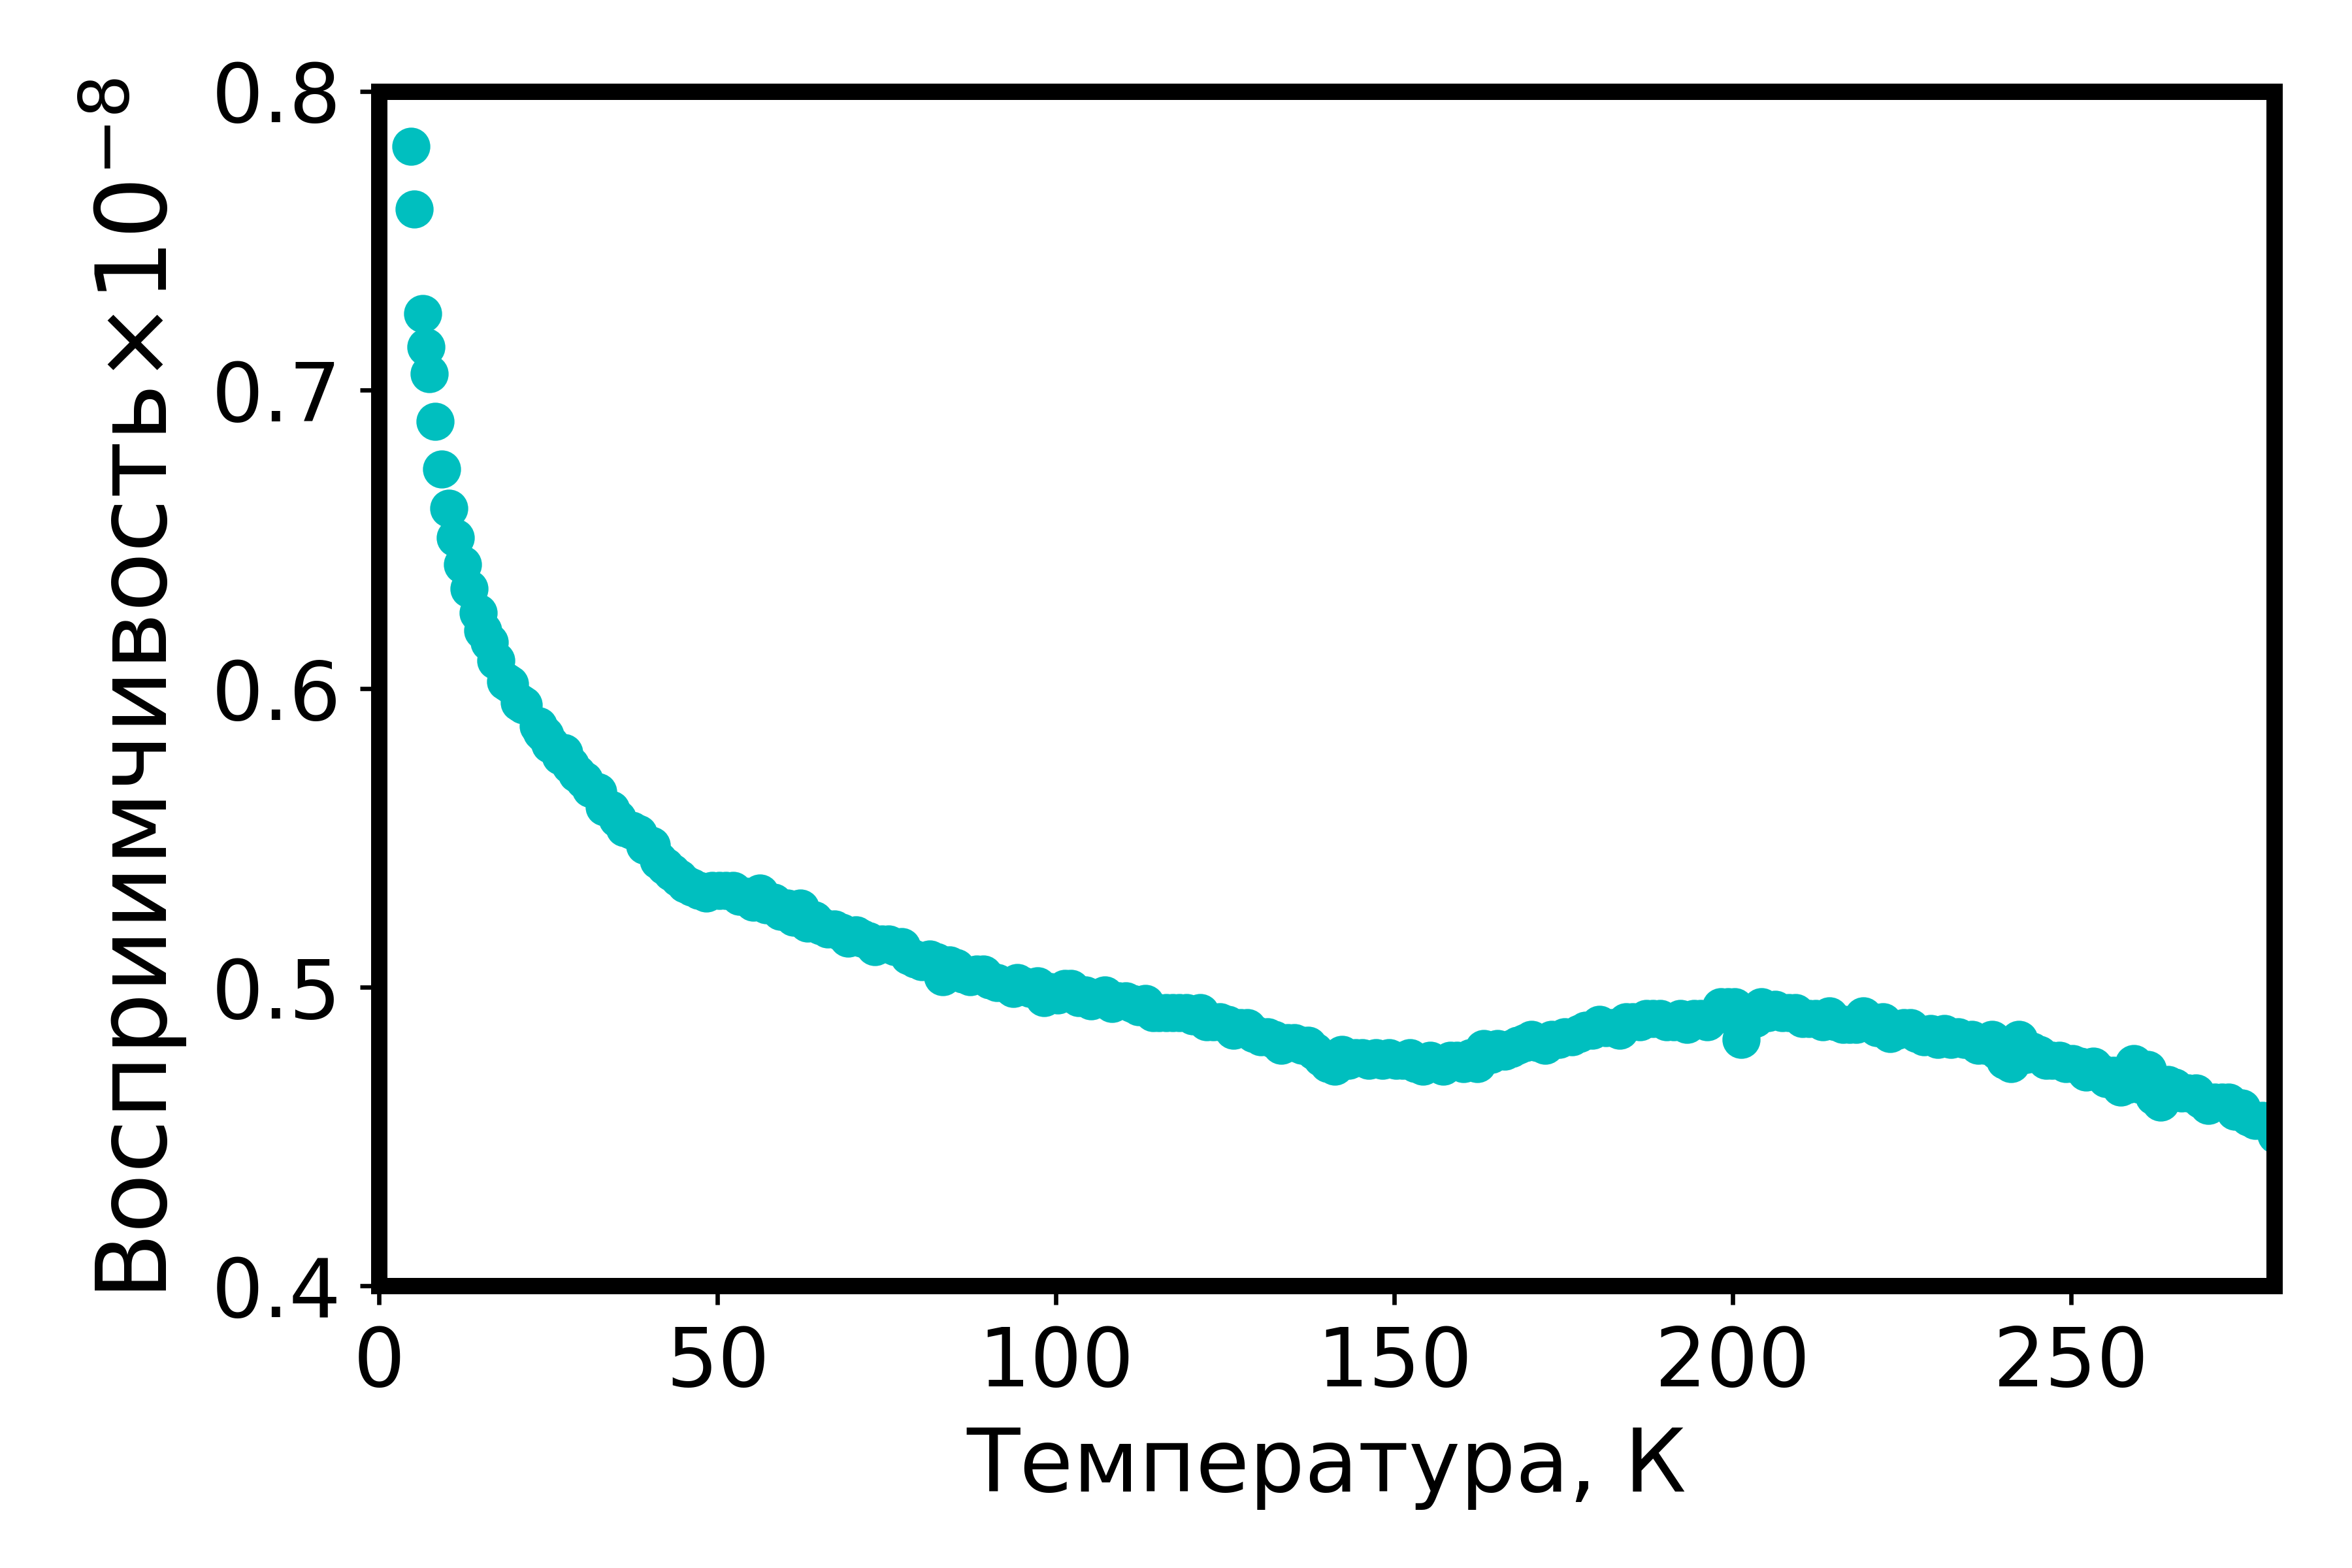
\includegraphics[width=0.9\linewidth]{sus_exp_Cu_Sb_Se} \\ б)
  \end{minipage}
      \caption[Графики зависимости магнитной восприимчивости для образцов Cu\textsubscript{12}Sb\textsubscript{4}S\textsubscript{13} (а) и Cu\textsubscript{3}SbSe\textsubscript{3} (б)]{Графики зависимости магнитной восприимчивости для образцов Cu\textsubscript{12}Sb\textsubscript{4}S\textsubscript{13} (а) и Cu\textsubscript{3}SbSe\textsubscript{3} (б)}
    \label{img:magsus2}
\end{figure}

График зависимости для монокристаллического образца Cu\textsubscript{12}Sb\textsubscript{4}S\textsubscript{13} в диапазоне температур от 2 до 100 К имеет вид отличный от кривой Кюри"--~Вейса.
 Характер кривой измеренной магнитной восприимчивости образца  Cu\textsubscript{12}Sb\textsubscript{4}S\textsubscript{13}, показывает наличие возможного перехода из парамагнитного состояния в антиферромагнитное в диапазоне температур от 80 до 90~К (\ref{img:magsus1}а).
До температуры 100 К зависимость парамагнитного вклада магнитной восприимчивости монотонно возрастает с понижением температуры и согласуется с Кюри"--~Вейсовским поведением, характерным для парамагнетика.

График зависимости удельной намагниченности образца Cu\textsubscript{3}SbS\textsubscript{3} от температуры представлен на рис. \ref{img:magsus1}б.
В интервале температур 170--200~К происходит рост магнитной восприимчивости, а в диапазоне температур 50--150~К наблюдается отклонение от парамагнитного поведения описываемого Кюри"--~Вейсовским законом.
Предположительно, в интервале температур 50--200 К реализуется особое магнитное состояние в соединении синтетического Мгриита.


По"~видимому, в данных интервалах температур реализуется особое магнитное состояние, которое связывается с искажением тетраэдрических комплексов в структуре.

\newpage


\section{Температурная зависимость теплоёмкости Cu\textsubscript{12}As\textsubscript{4}S\textsubscript{13} и Cu\textsubscript{3}AsSe\textsubscript{3}} \label{sect3_4}
На рис. \ref{img:heat} представлена экспериментальная и теоретическая зависимость теплоемкости  образца от температуры, полученная методом релаксации теплового импульса для образцов Сu\textsubscript{12}As\textsubscript{4}S\textsubscript{13} и Cu\textsubscript{3}AsSe\textsubscript{3}.
На рисунке \ref{img:heat}(а) представлена экспериментальная зависимость теплоёмкости от температуры для синтетического теннантита Сu\textsubscript{12}As\textsubscript{4}S\textsubscript{13}. На графике функции наблюдаются отклонения от нормального хода теплоёмкости в диапазоне от 150 до 190 и при 285~К. Синим цветом обозначена расчетная функция теплоёмкости от температуры с тремя дополнительными осцилляторами Эйнштейна. Температура Дебая для Cu\textsubscript{12}As\textsubscript{4}S\textsubscript{13} составляет 623~К, характерные температуры эйнштейновских осцилляторов, которые составляют 65, 124 и 220~К. Температура 65~К соответствует энергии активации спин-решеточной флуктуации\cite{Gainov2008,Gainov_2006}, 124~К "--- характерному максимуму на графике зависимости магнитной восприимчивости и изменению параметра атомного смещения для позиции S(2), 220~К "--- особенностям температурной зависимости коэффициента упругой податливости\cite{bab_81}.

На рисунке \ref{img:heat}(б) представлена экспериментальная зависимость теплоёмкости от температуры для синтетического теннантита Сu\textsubscript{12}As\textsubscript{4}S\textsubscript{13}. На графике функции наблюдаются отклонения от нормального хода теплоёмкости в диапазоне от 150 до 190 и при 285 К. Синим цветом обозначена расчетная функция теплоёмкости от температуры с тремя дополнительными осцилляторами Эйнштейна. Температура Дебая для Cu\textsubscript{3}AsSe\textsubscript{3} составляет 500~К, характерные температуры эйнштейновских осцилляторов, которые составляют 42, 186 и 288~К.   Температуры 186 и 288~К соответствуют характерным максимумам на графике зависимости магнитной восприимчивости и  особенностям температурной зависимости коэффициента упругой податливости \cite{bab_81}.

\begin{figure}[p!]
  \begin{minipage}[ht]{0.9\linewidth}\centering
    \includegraphics[width=0.9\linewidth]{Heat_capacity_Cu12As4S13} \\ а)
  \end{minipage}
  \vfill
  \begin{minipage}[ht]{0.9\linewidth}\centering
    \includegraphics[width=0.9\linewidth]{Heat_capacity_Cu3AsSe3} \\ б)
  \end{minipage}

      \caption[Зависимость теплоемкости образцов Cu\textsubscript{12}As\textsubscript{4}S\textsubscript{13} (а) и Cu\textsubscript{3}AsS\textsubscript{3} (б) от температуры. Точки~"---экспериментальные данные, сплошная линия~"---модельные значения теплоемкости]{Зависимость теплоемкости образцов Cu\textsubscript{12}As\textsubscript{4}S\textsubscript{13} (а) и Cu\textsubscript{3}AsS\textsubscript{3} (б) от температуры. Точки~"---экспериментальные данные, сплошная линия~"---модельные значения теплоемкости}
    \label{img:heat}
\end{figure}



\newpage

\section{Спектры комбинационного рассеяния} \label{sect3_5}

Спектры комбинационного рассеяния для исследованных соединений обладают низкоэнергетическими модами (Рис. \ref{img:raman1} и \ref{img:raman2}).
В таблице \ref{tabl_raman} представлены определенные по экспериментальным спектрам положения пиков для исследуемых соединений и их полуширина.
Следует отметить, что энергия пиков для соединения Cu\textsubscript{12}Sb\textsubscript{4}S\textsubscript{13} составляет 8.5  и 12~мэВ, что находится в хорошем согласии с теоретическими\cite{Lai_2015} и экспериментальными\cite{May2016} опубликованными данными.

\begin{table} [htbp]%
    \centering
	\caption{Положение пиков на спектрах комбинационного рассеяния и их полуширина для сложных соединений халькогенидов меди}%
	\label{tabl_raman}% label всегда желательно идти после caption
    \renewcommand{\arraystretch}{1.5}
	\begin{tabular}{@{}@{\extracolsep{20pt}}lllll@{}}
        \toprule     %%% верхняя линейка
    	 & \multicolumn{3}{c}{положение пика и  полуширина, см\textsuperscript{-1}}& \\
        \midrule
    Cu\textsubscript{12}As\textsubscript{4}S\textsubscript{13} & 67 (14)	 &122 (24) 											& & 	\\ \hline
   Cu\textsubscript{3}AsSe\textsubscript{3}&  155 (7)				& 200 (37)						&254 (6) 	&  \\ \hline
    	 Cu\textsubscript{12}Sb\textsubscript{4}S\textsubscript{13} 	& 69 (20)	& 97 (11) 	& 		& 	\\ \hline
    	 Cu\textsubscript{3}SbSe\textsubscript{3}	 	& 110 (14)				& 148 (11) 	& 205 (25)		& \\ \hline
        \bottomrule
	\end{tabular}%
\end{table}

Определение положения  и  полуширины пика проведено с помощью псевдо-функции  Фойгта.
Модель аппроксимации  основана на псевдо-функциях Фойгта для каждого пика и полиномной функции для фона.

\begin{figure}[p!]
  \begin{minipage}[ht]{0.9\linewidth}\centering
    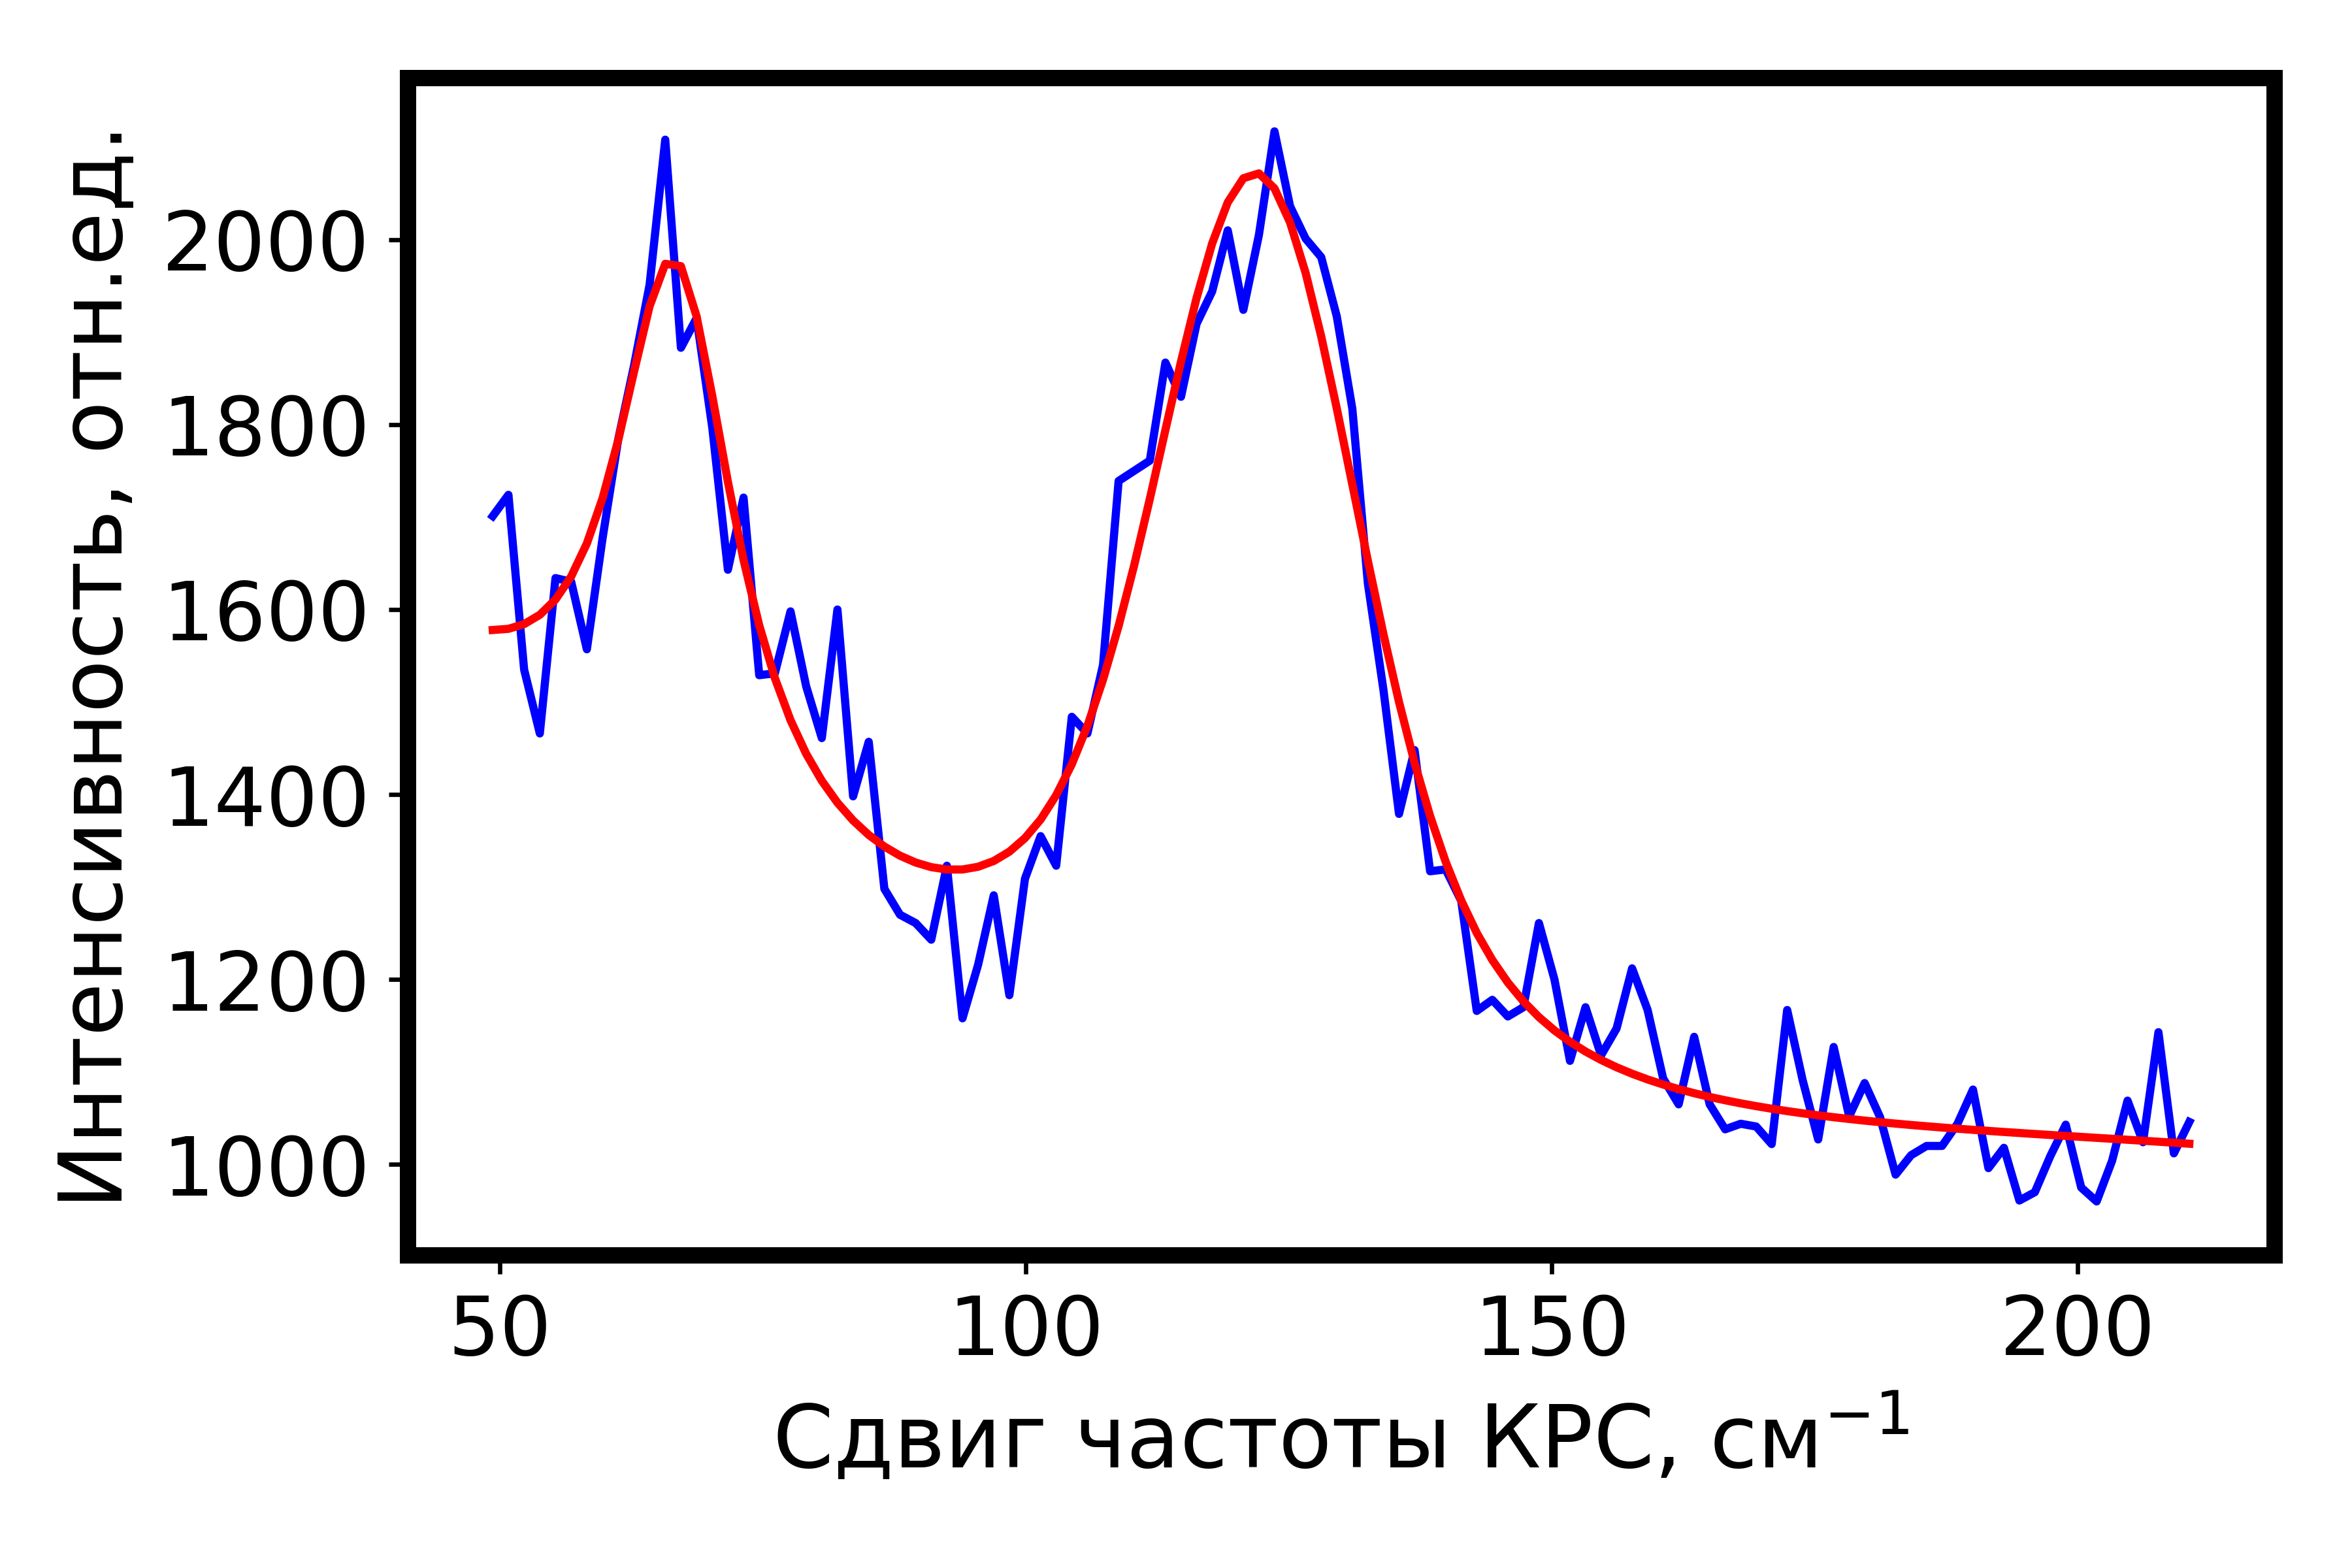
\includegraphics[width=0.9\linewidth]{raman_25_CuAsS3} \\ а)
  \end{minipage}
  \vfill
  \begin{minipage}[ht]{0.9\linewidth}\centering
    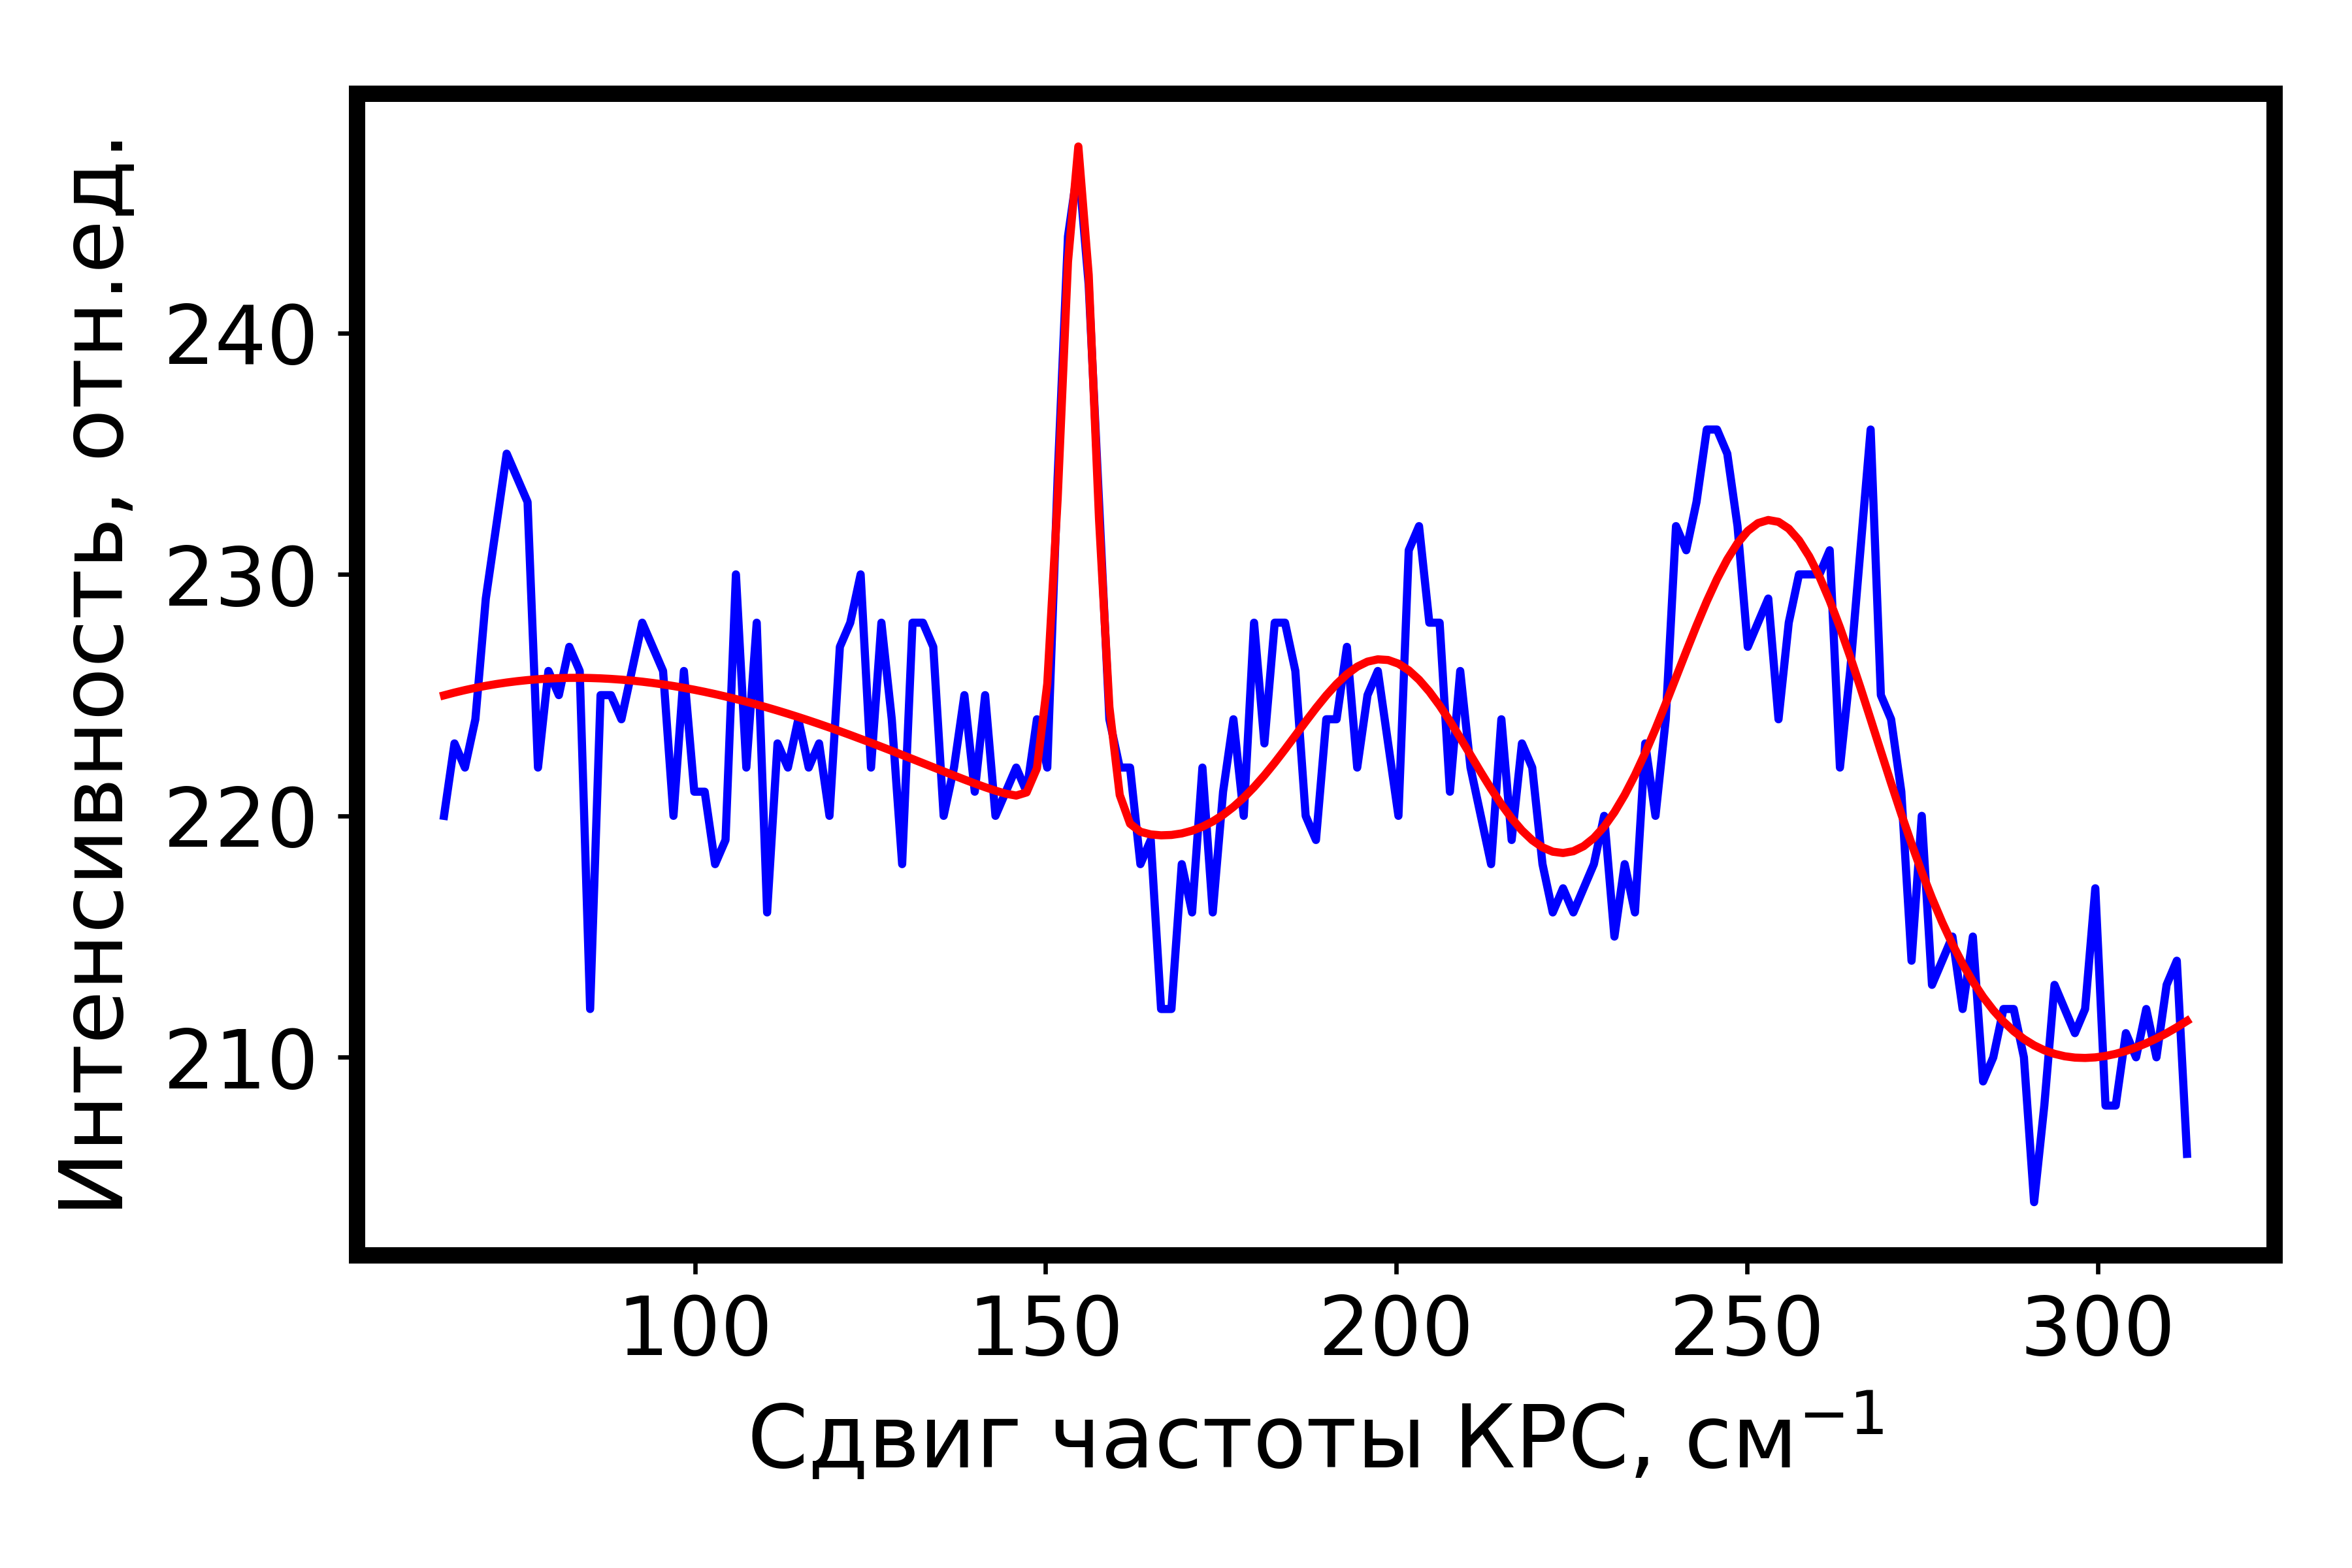
\includegraphics[width=0.9\linewidth]{raman_288_Cu3AsSe3} \\ б)
  \end{minipage}

      \caption[Графики спектров комбинационного рассеяния соединений Cu\textsubscript{12}As\textsubscript{4}S\textsubscript{13} (а) и  Cu\textsubscript{3}AsSe\textsubscript{3} (б)]{Графики спектров комбинационного рассеяния соединений Cu\textsubscript{12}As\textsubscript{4}S\textsubscript{13} (а) и  Cu\textsubscript{3}AsSe\textsubscript{3} (б)}
    \label{img:raman1}
\end{figure}

\begin{figure}[p!]
  \begin{minipage}[ht]{0.9\linewidth}\centering
    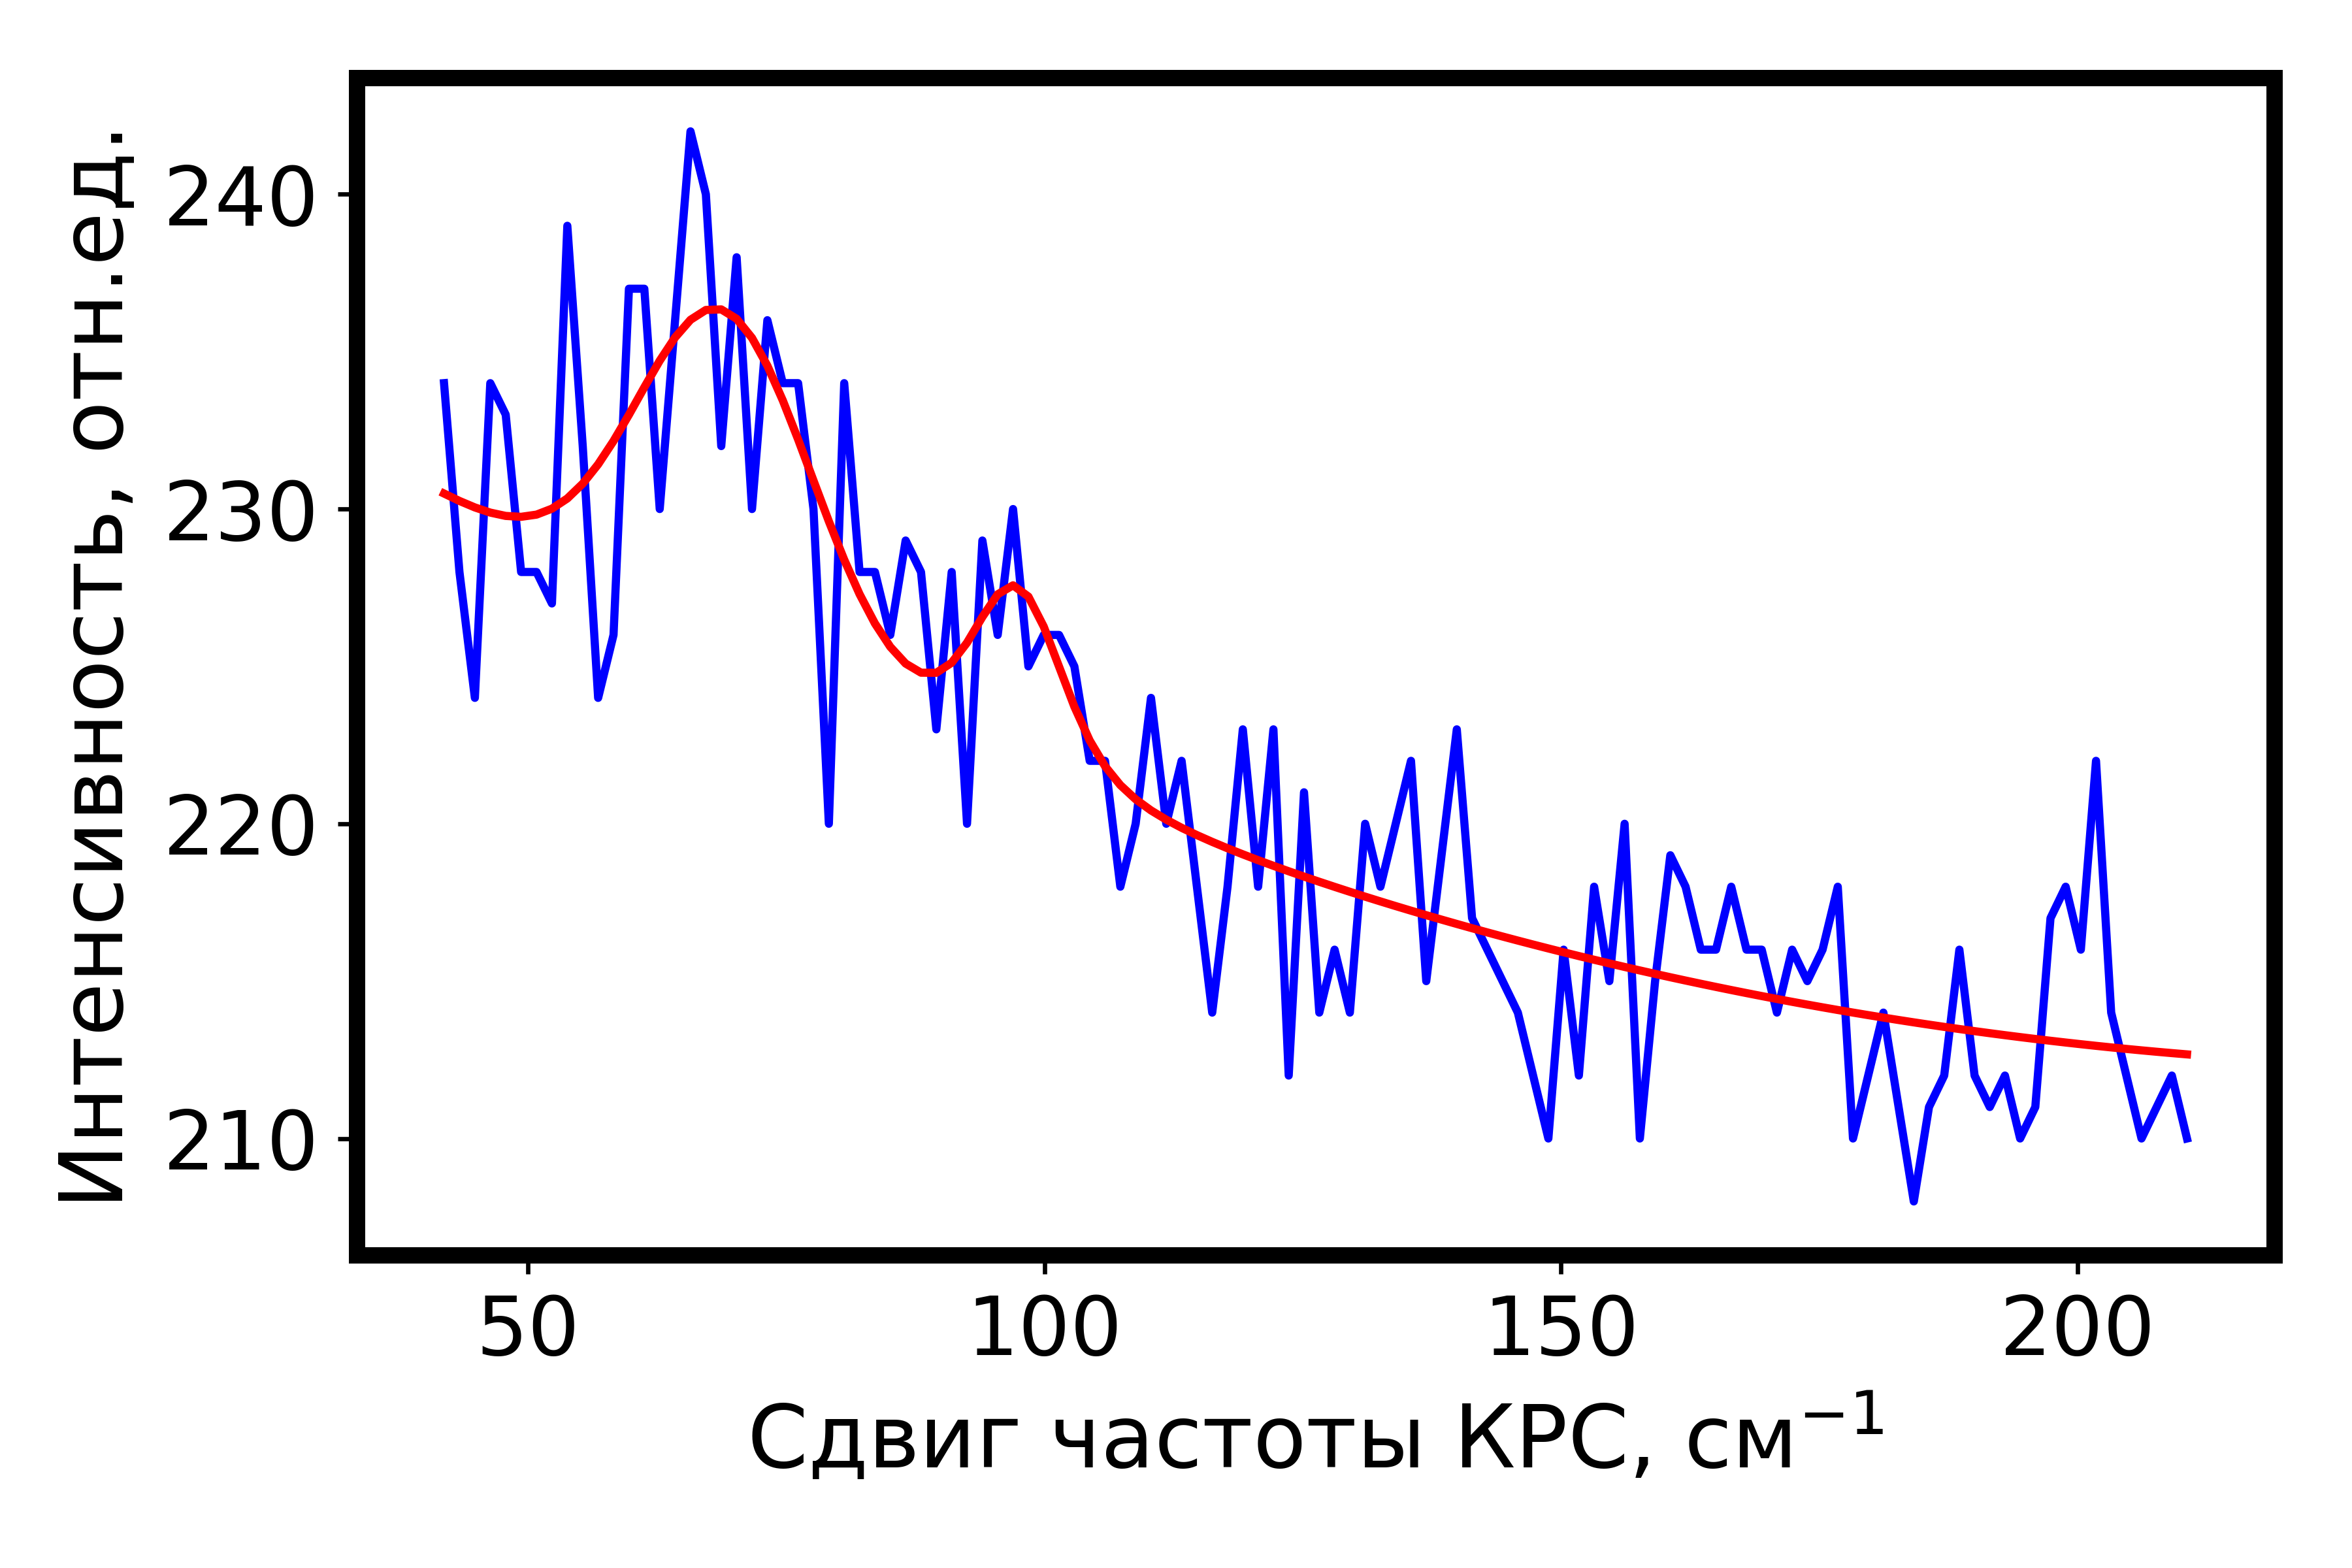
\includegraphics[width=0.9\linewidth]{raman_206_Cu3SbS3} \\ а)
  \end{minipage}
  \vfill
  \begin{minipage}[ht]{0.9\linewidth}\centering
    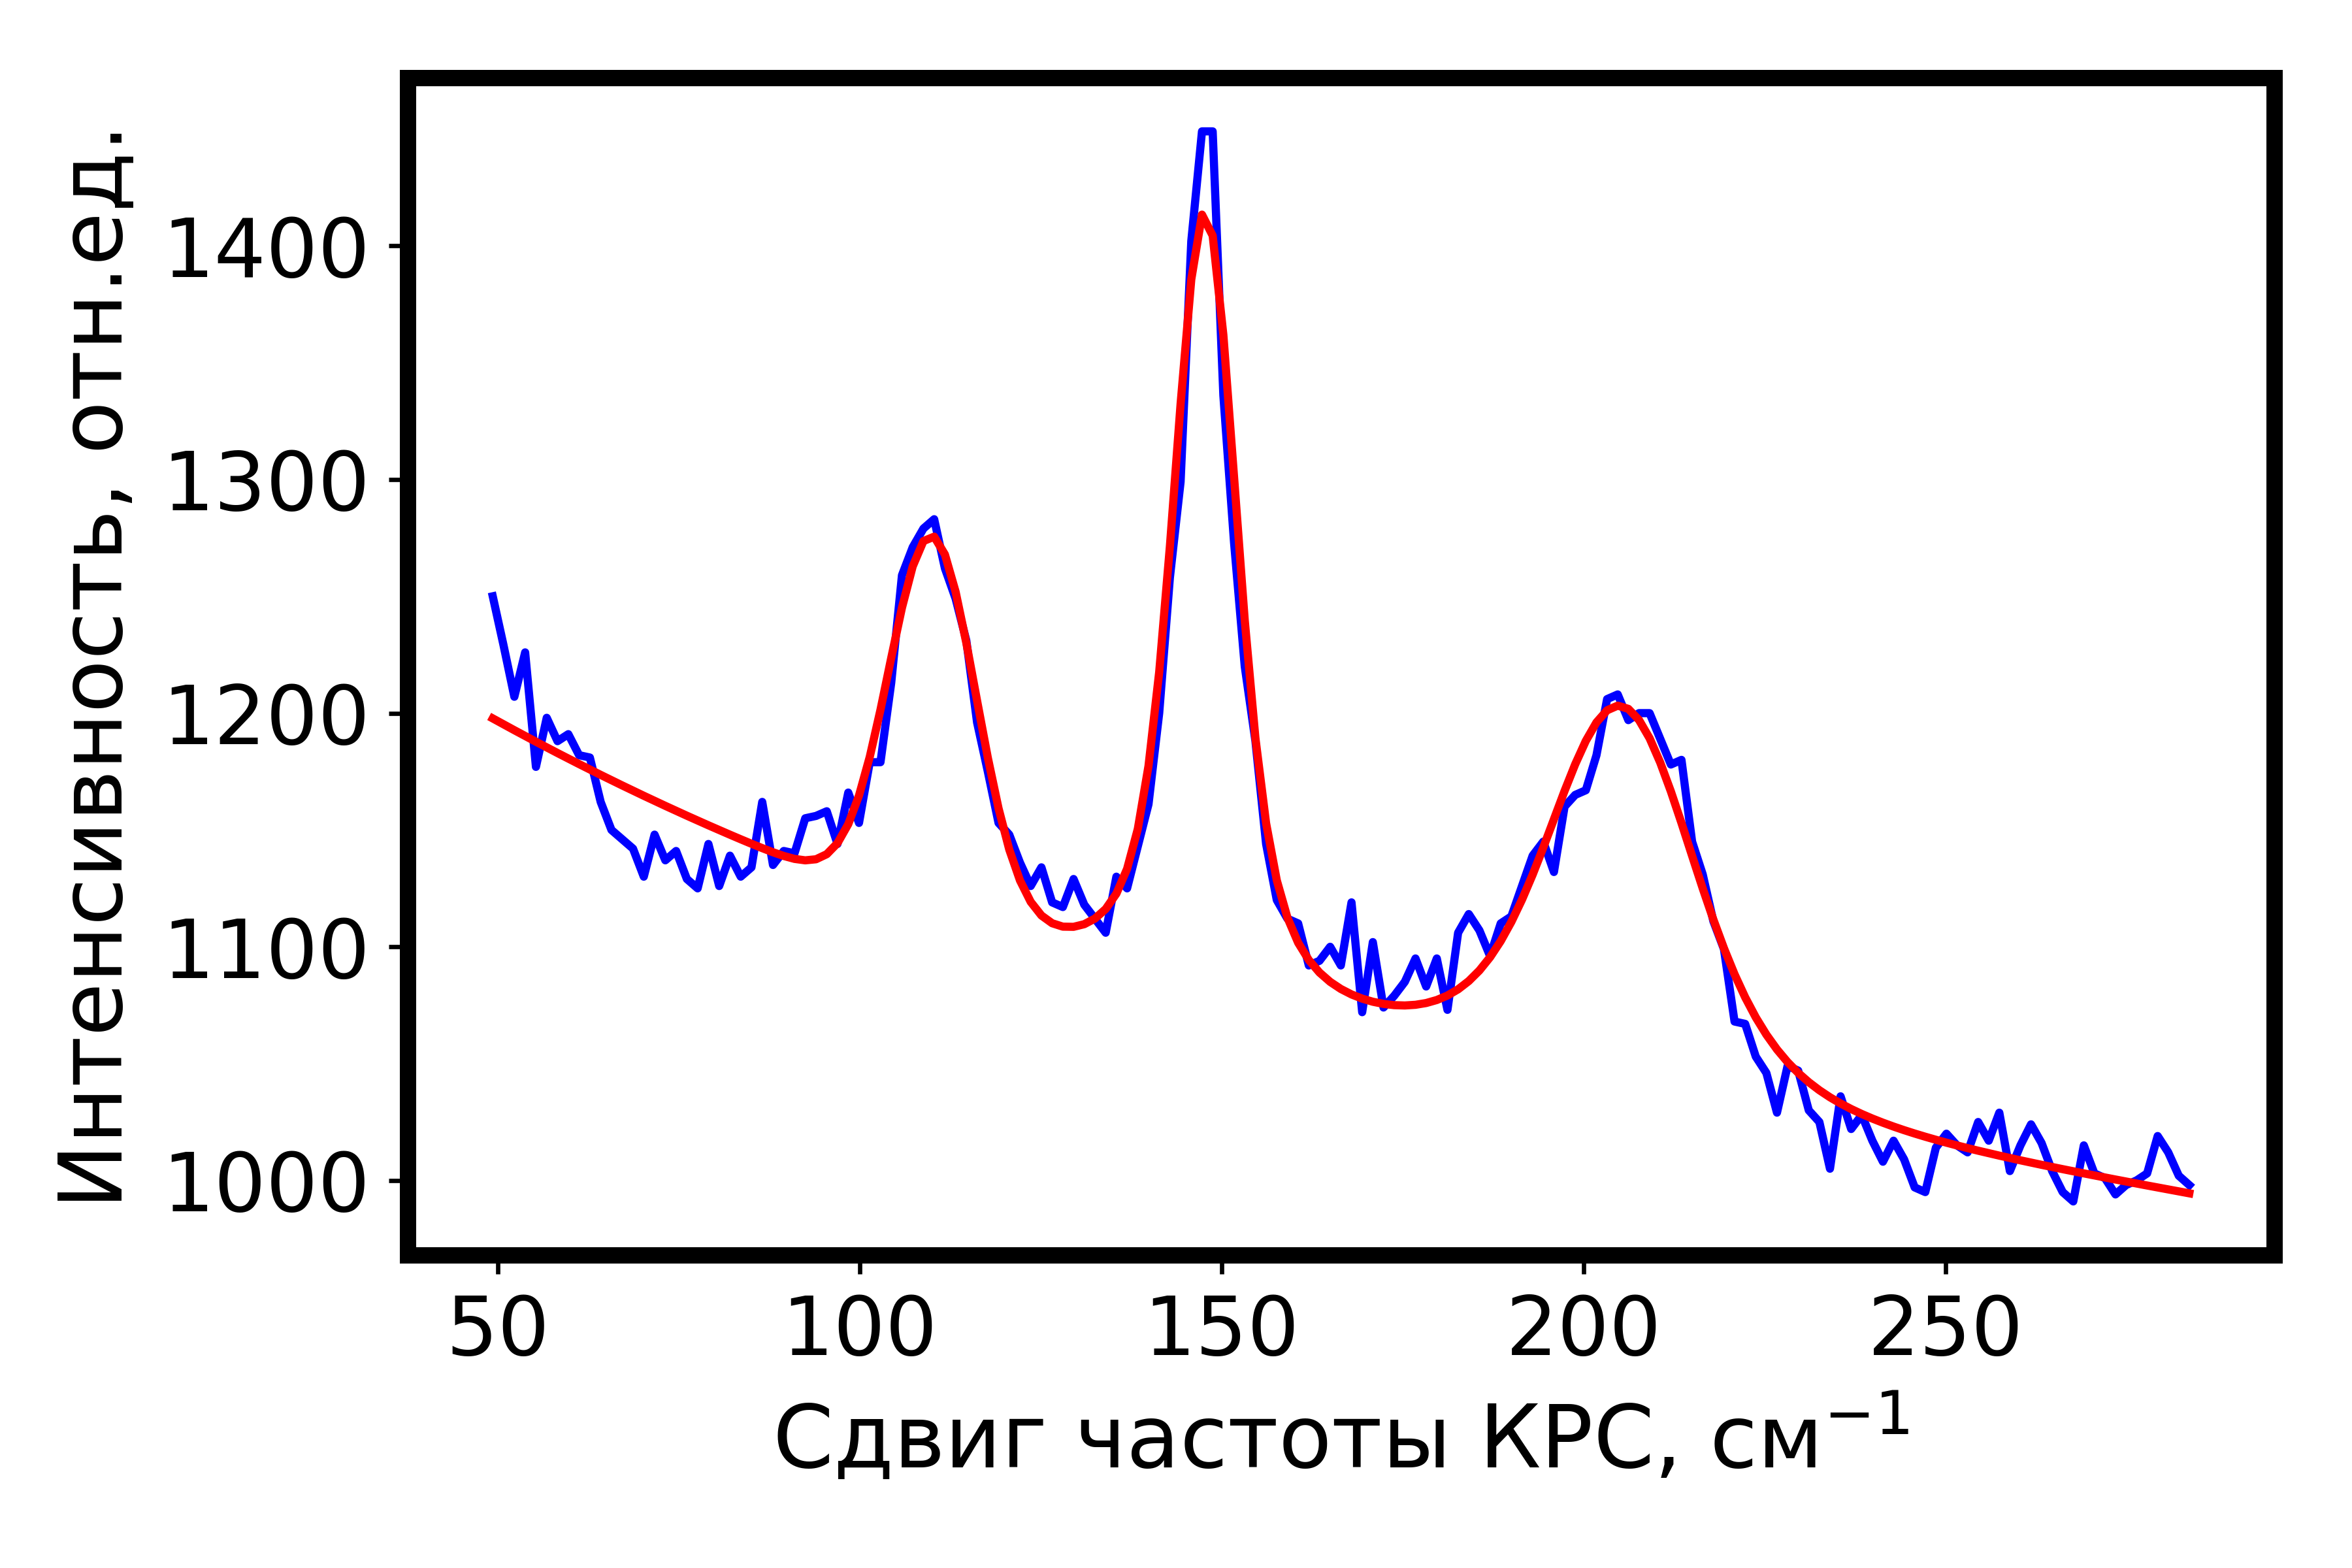
\includegraphics[width=0.9\linewidth]{raman_209_Cu3SbSe3} \\ б)
  \end{minipage}

      \caption[Графики спектров комбинационного рассеяния соединений Cu\textsubscript{12}Sb\textsubscript{4}S\textsubscript{13} (а) и Cu\textsubscript{3}SbSe\textsubscript{3} (б)]{Графики спектров комбинационного рассеяния соединений Cu\textsubscript{12}Sb\textsubscript{4}S\textsubscript{13} (а) и Cu\textsubscript{3}SbSe\textsubscript{3} (б)}
    \label{img:raman2}
\end{figure}


\newpage


\section{Квантовомеханическое расчеты} \label{sect3_6}

Для исследования наиболее выгодного положения атомов меди были рассчитаны энергии 20 структур с разным положением атомов меди.
Структуры разделены на две группы: первая --- в лавесовском полиэдре сдвинуты 6 атомов меди (структуры с 1 по 10), и вторая --- сдвинуты 3 атома меди в лавесовском полиэдре (структуры с 10 по 19). Изображения рассчитанных структур представлены на рисунках \ref{img:laves1}, \ref{img:laves2}, \ref{img:laves3} и \ref{img:laves4}.
На рисунке \ref{img:th} представлен график со значениями энергий элементарных ячеек для рассчитанных структур. Красной пунктирной линией обозначена энергия исходной структуры.
Экспериментальные структуры, полученные после анализа рентгеноструктурных экспериментов при разных температурах, были обсчитаны с учетом ферромагнитного, антиферромагнитного, парамагнитного (ПМ) и диамагнитного упорядочений в структурах.
Антиферромагнитное упорядочение в экспериментальной структуре при 85~К энергетически более выгодно, чем ферро- или пара- или диамагнитное состояние. При этом для 293~К ФМ, АФМ, ПМ конфигурации имеют одинаковую до 4 знака энергию, что указывает на их одинаковую выгодность.

\begin{figure}[ht!]
  \begin{minipage}[ht]{0.9\linewidth}\centering
    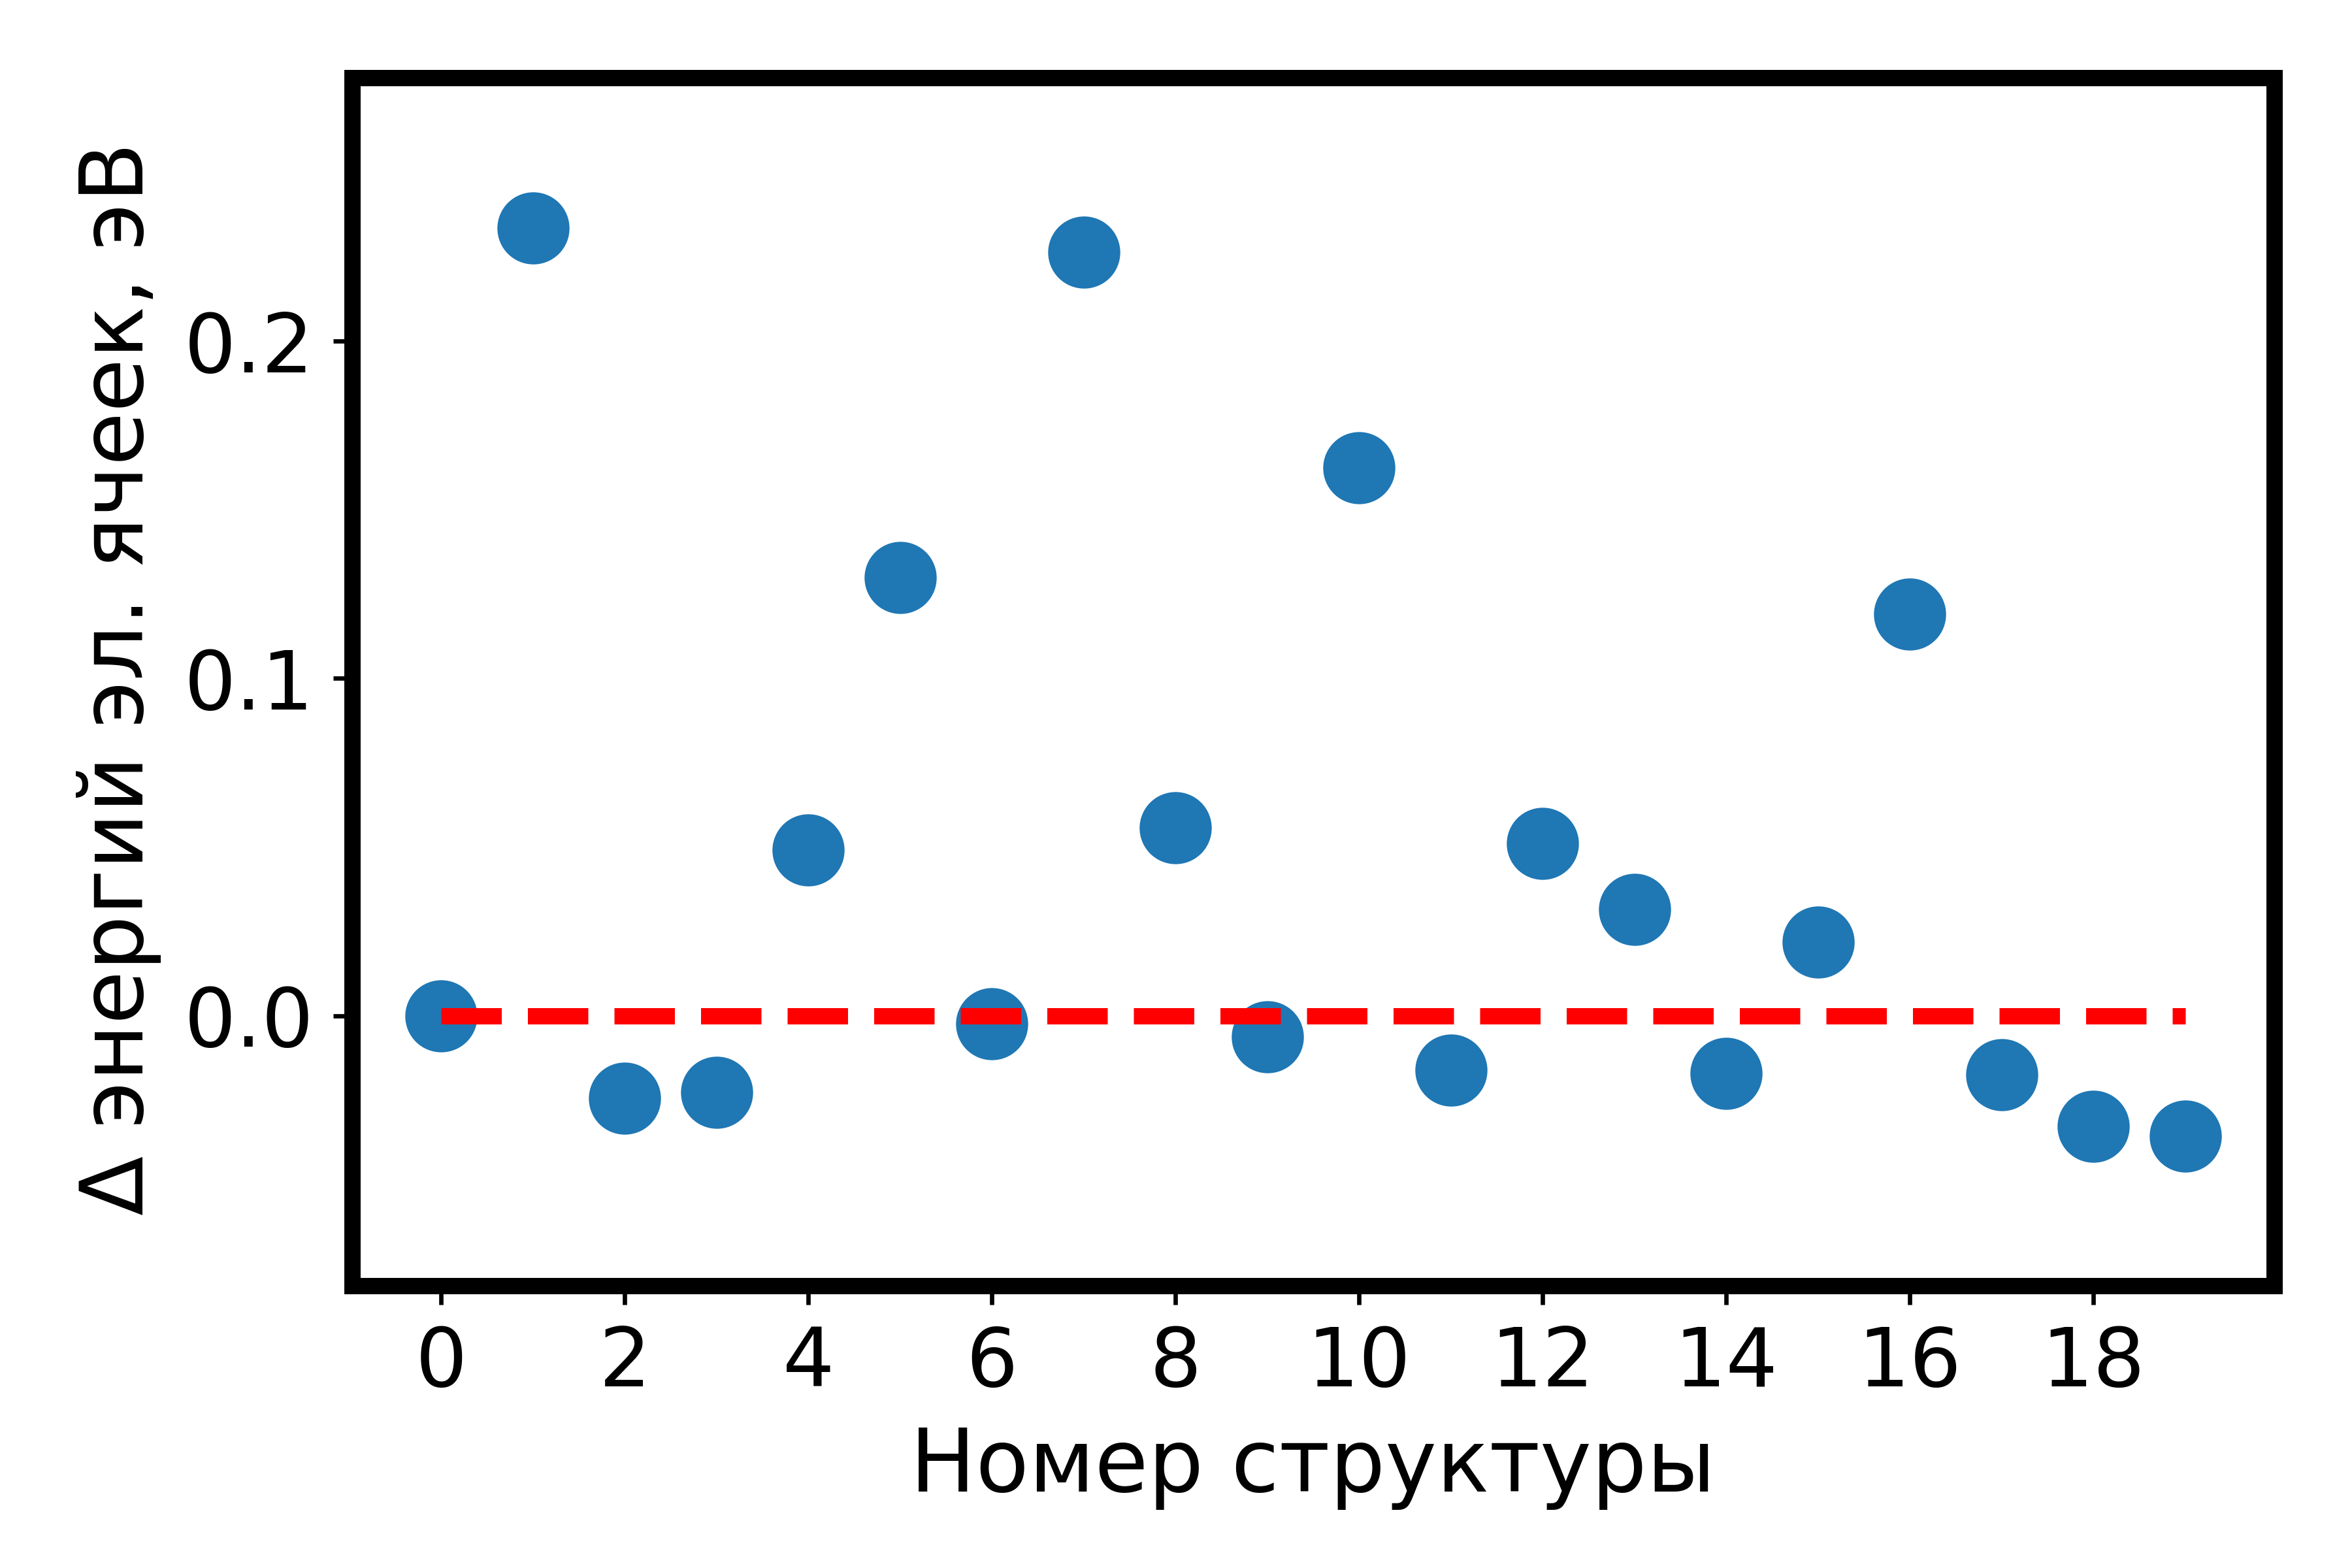
\includegraphics[width=0.7\linewidth]{energy_structure}
  \end{minipage}

      \caption[Сводный график энергий рассчитанных структур, с разным расположением атомов в лавесовском полиэдре]{Сводный график энергий рассчитанных структур, с разным расположением атомов в лавесовском полиэдре}
    \label{img:th}
\end{figure}

\begin{landscape}
\begin{table} [htbp]
\centering

\caption{Сводная таблица распределения электрических зарядов для рассчитанных структур (варианты с 0 по 9 включительно) с разным расположением атомов меди в лавесовском полиэдре для синтетического теннантита Cu\textsubscript{12}As\textsubscript{4}S\textsubscript{13}}%
	\label{mod_char1}% label всегда желательно идти после caption
    \renewcommand{\arraystretch}{1.5}
	%\resizebox{\textwidth}{!}{
    \begin{tabular}{@{}@{\extracolsep{10pt}}lllllllllll@{}}
      \toprule     %%% верхняя линейка
Atom & Var0          & Var1          & Var2          & Var3          & Var4   & Var5          & Var6          & Var7          & Var8          & Var9              \\  \midrule
\multirow{2}{*}{Cu1} & \multirow{2}{*}{+0.557}  &\multirow{2}{*}{+0.554}& \multirow{2}{*}{+0.556} & \multirow{2}{*}{+0.555} & +0.557 & \multirow{2}{*}{+0.554}  & \multirow{2}{*}{+0.553}  & \multirow{2}{*}{+0.555}  & \multirow{2}{*}{+0.555}& \multirow{2}{*}{+0.555} \\
&&&&&+0.547&&&&&\\ \hline
\multirow{2}{*}{Cu2} & \multirow{2}{*}{+0.497}  & +0.481 & +0.453  & +0.483 & +0.521 & +0.502 & +0.485  & +0.508  & +0.504  & +0.504    \\
				                             & &  +0.456 &  +0.394 &+0.381 &  +0.464 & +0.386 &+0.433 & +0.434 &+0.429 & +0.429  \\ \hline
\multirow{2}{*}{S1}   & -1.479 & -1.512 & -1.498 &-1.488 & -0.744 &  -1.421 & -1.388  & -1.404  & -1.411 & -1.411    \\
                              &-1.479 & -1.512 &-1.498 & -1.488 & -0.744  & -1.519 & -1.515 & -1.531 & -1.541 &  -1.541   \\ \hline
S2   & -0.976        & -0.886        & -0.777        & -0.803        & -0.926   & -0.850        & -0.873        & -0.888        & -0.930        & -0.930          \\ \hline
\multirow{2}{*}{As}   & \multirow{2}{*}{+3.001} & +3.045  & +3.103  & +3.046  & +0.905&  +3.012 &  +3.010 & +2.994 & +2.992 &  +2.992     \\
&  & +3.014 & +2.993 &+3.175 & +0.853&+3.012 & +3.010 &  +2.994 &+2.992 & +2.992 \\ \hline
\bottomrule

\end{tabular}
%}
\end{table}
\end{landscape}

\begin{landscape}
\begin{table} [htbp]
\centering
\caption{Сводная таблица распределения электрических зарядов для рассчитанных структур (варианты с 10 по 19 включительно) с разным расположением атомов меди в лавесовском полиэдре для синтетического теннантита Cu\textsubscript{12}As\textsubscript{4}S\textsubscript{13}}%
	\label{mod_char2}% label всегда желательно идти после caption
    \renewcommand{\arraystretch}{1.5}
	\begin{tabular}{@{}@{\extracolsep{10pt}}lllllllllll@{}}

\toprule     %%% верхняя линейка
Atom                         &Var10& Var11& Var12& Var13 & Var14& Var15& Var16& Var17& Var18& Var19          \\ \hline
Cu1                           & +0.555& +0.554& +0.553 & +0.555&+0.555&+0.554& +0.553&+0.555&+0.555&+0.555\\ \hline
\multirow{2}{*}{Cu2 } & +0.463  & +0.507  & +0.467  & +0.499 & +0.509   & +0.502  & +0.485  & +0.508  & +0.504  & +0.504 \\
                                &+0.480 & +0.312 &  +0.432 &  +0.429 &  +0.362  &  +0.386 &  +0.433 & +0.434 &  +0.429 &  +0.429  \\ \hline
\multirow{2}{*}{S1}   & -0.694 & -1.397  & -1.395  & -1.403& -1.414 & -1.421 & -1.388& -1.404& -1.411  & -1.411  \\
                                & -0.746 & -1.528 & -1.523 &  -1.532 & -1.520  &-1.519 &-1.515 &-1.531 & -1.541 & -1.541  \\ \hline
S2                        & -0.851        & -0.809        & -0.848        & -0.900        & -0.832         & -0.850        & -0.873        & -0.888        & -0.930        & -0.930         \\ \hline
\multirow{2}{*}{As}   & +0.758 & +3.162 &+3.003 &+3.062 &+3.097  & +3.094 & +3.064 & +3.073 & +3.062& +3.062 \\
                               & +0.920 & +3.000 & +3.085 &+3.002 & +2.984  & +3.012 &+3.010 &+2.994 &+2.992 &+2.992  \\ \hline
 \bottomrule


\end{tabular}
\end{table}
\end{landscape}

\begin{figure}[p!]
  \begin{minipage}[ht]{0.45\linewidth}\centering
    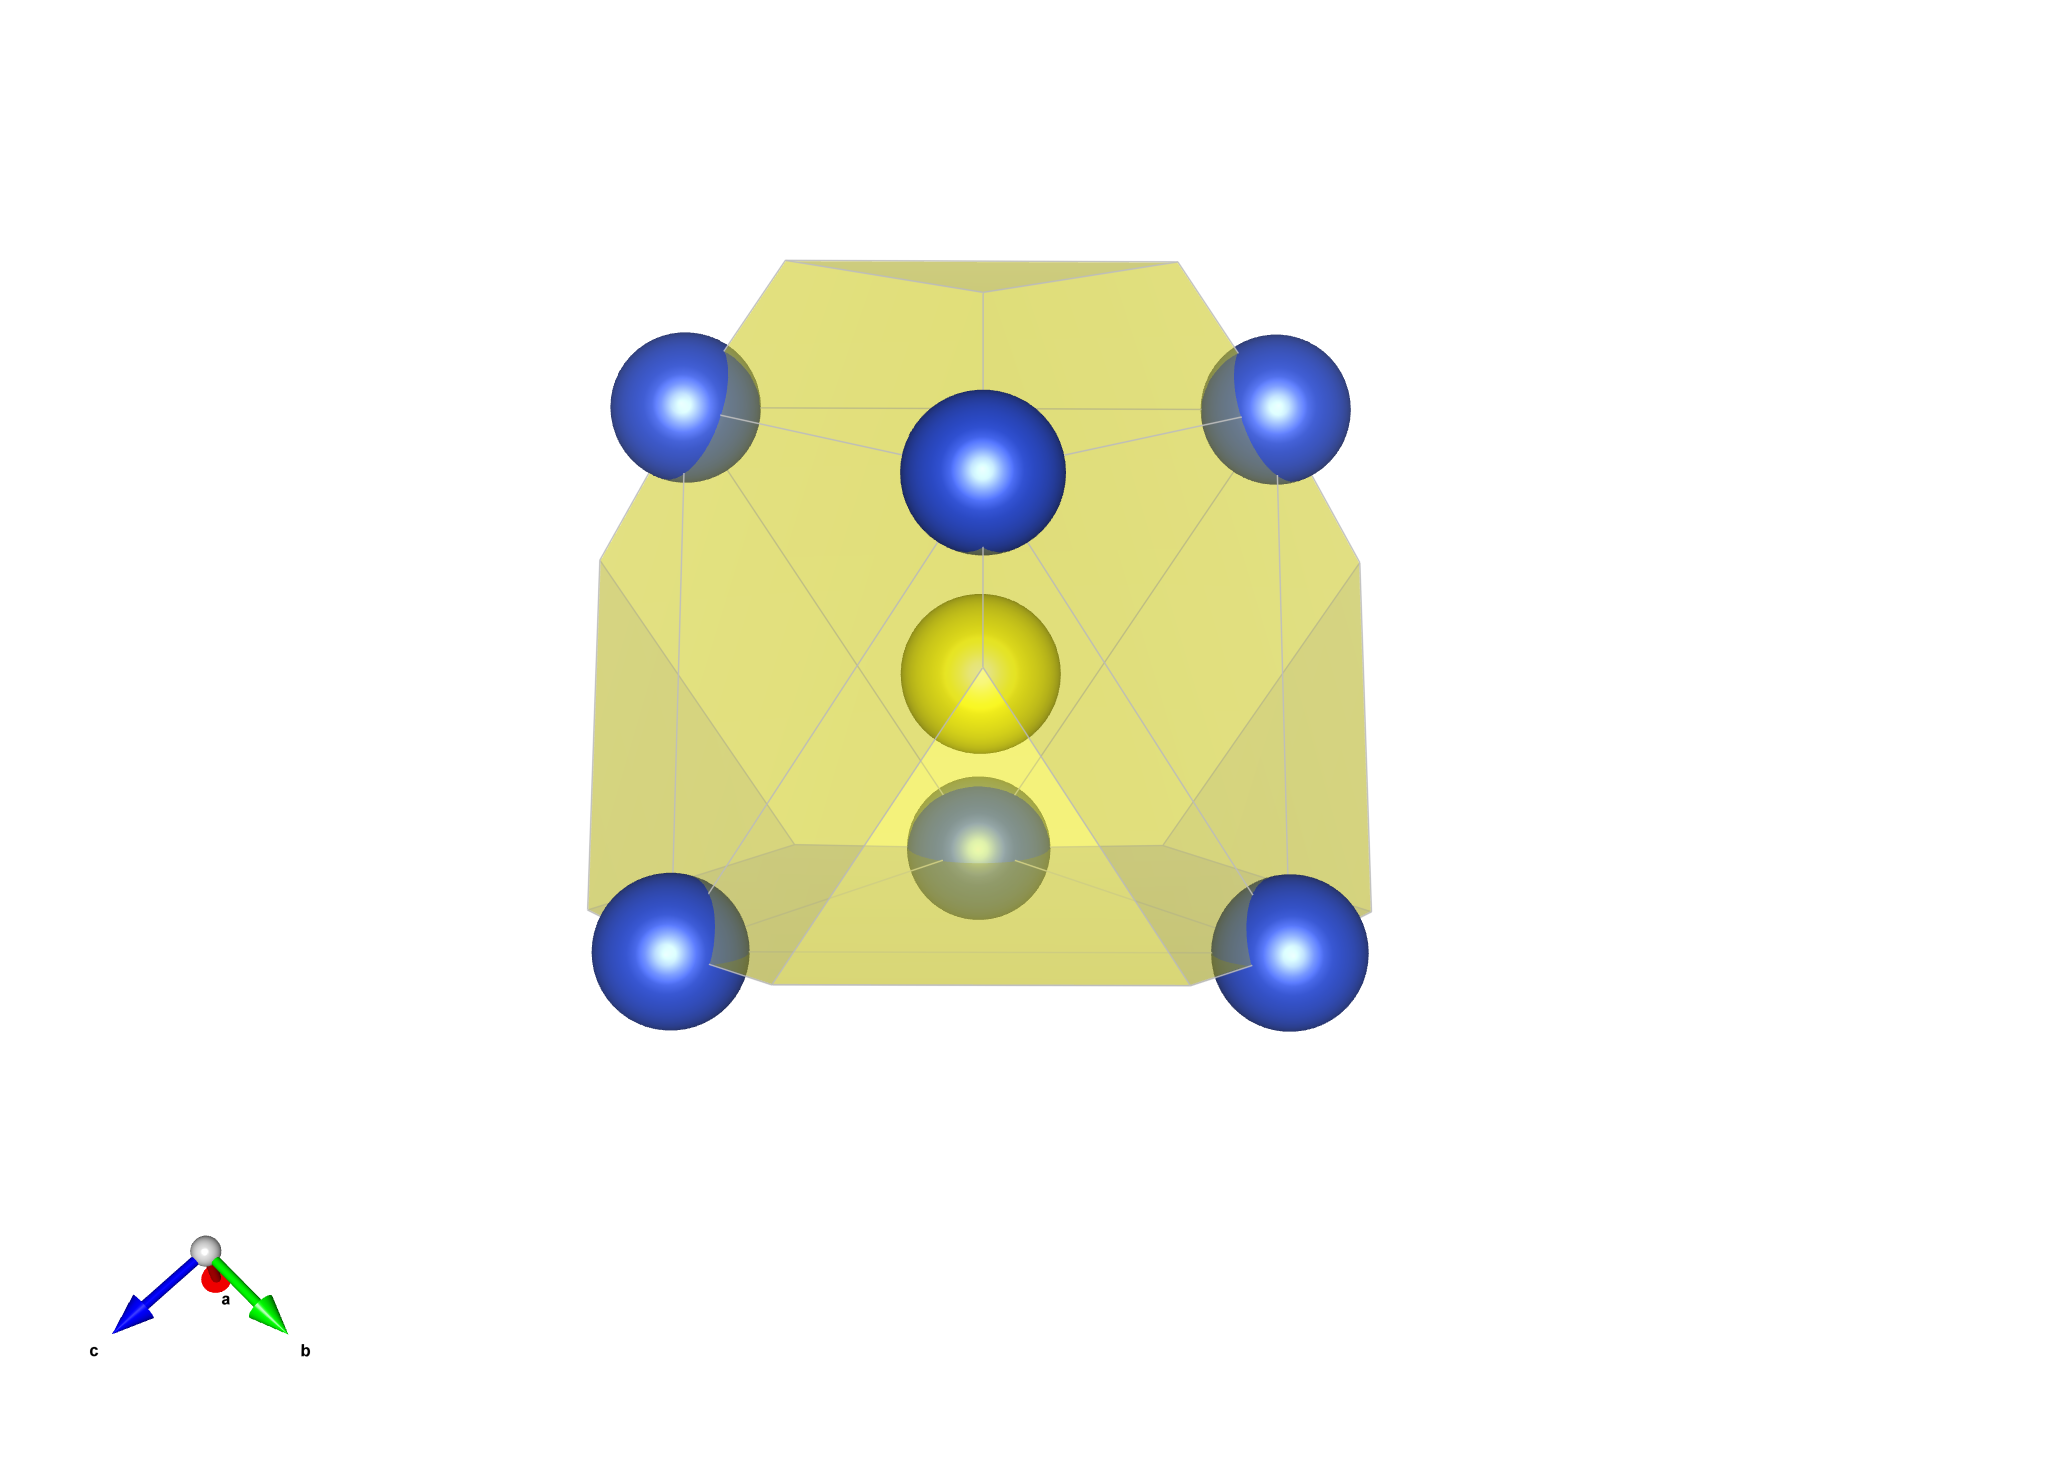
\includegraphics[width=0.9\linewidth]{var_0} \\ а)
  \end{minipage}
						\hfill
 \begin{minipage}[ht]{0.45\linewidth}\centering
    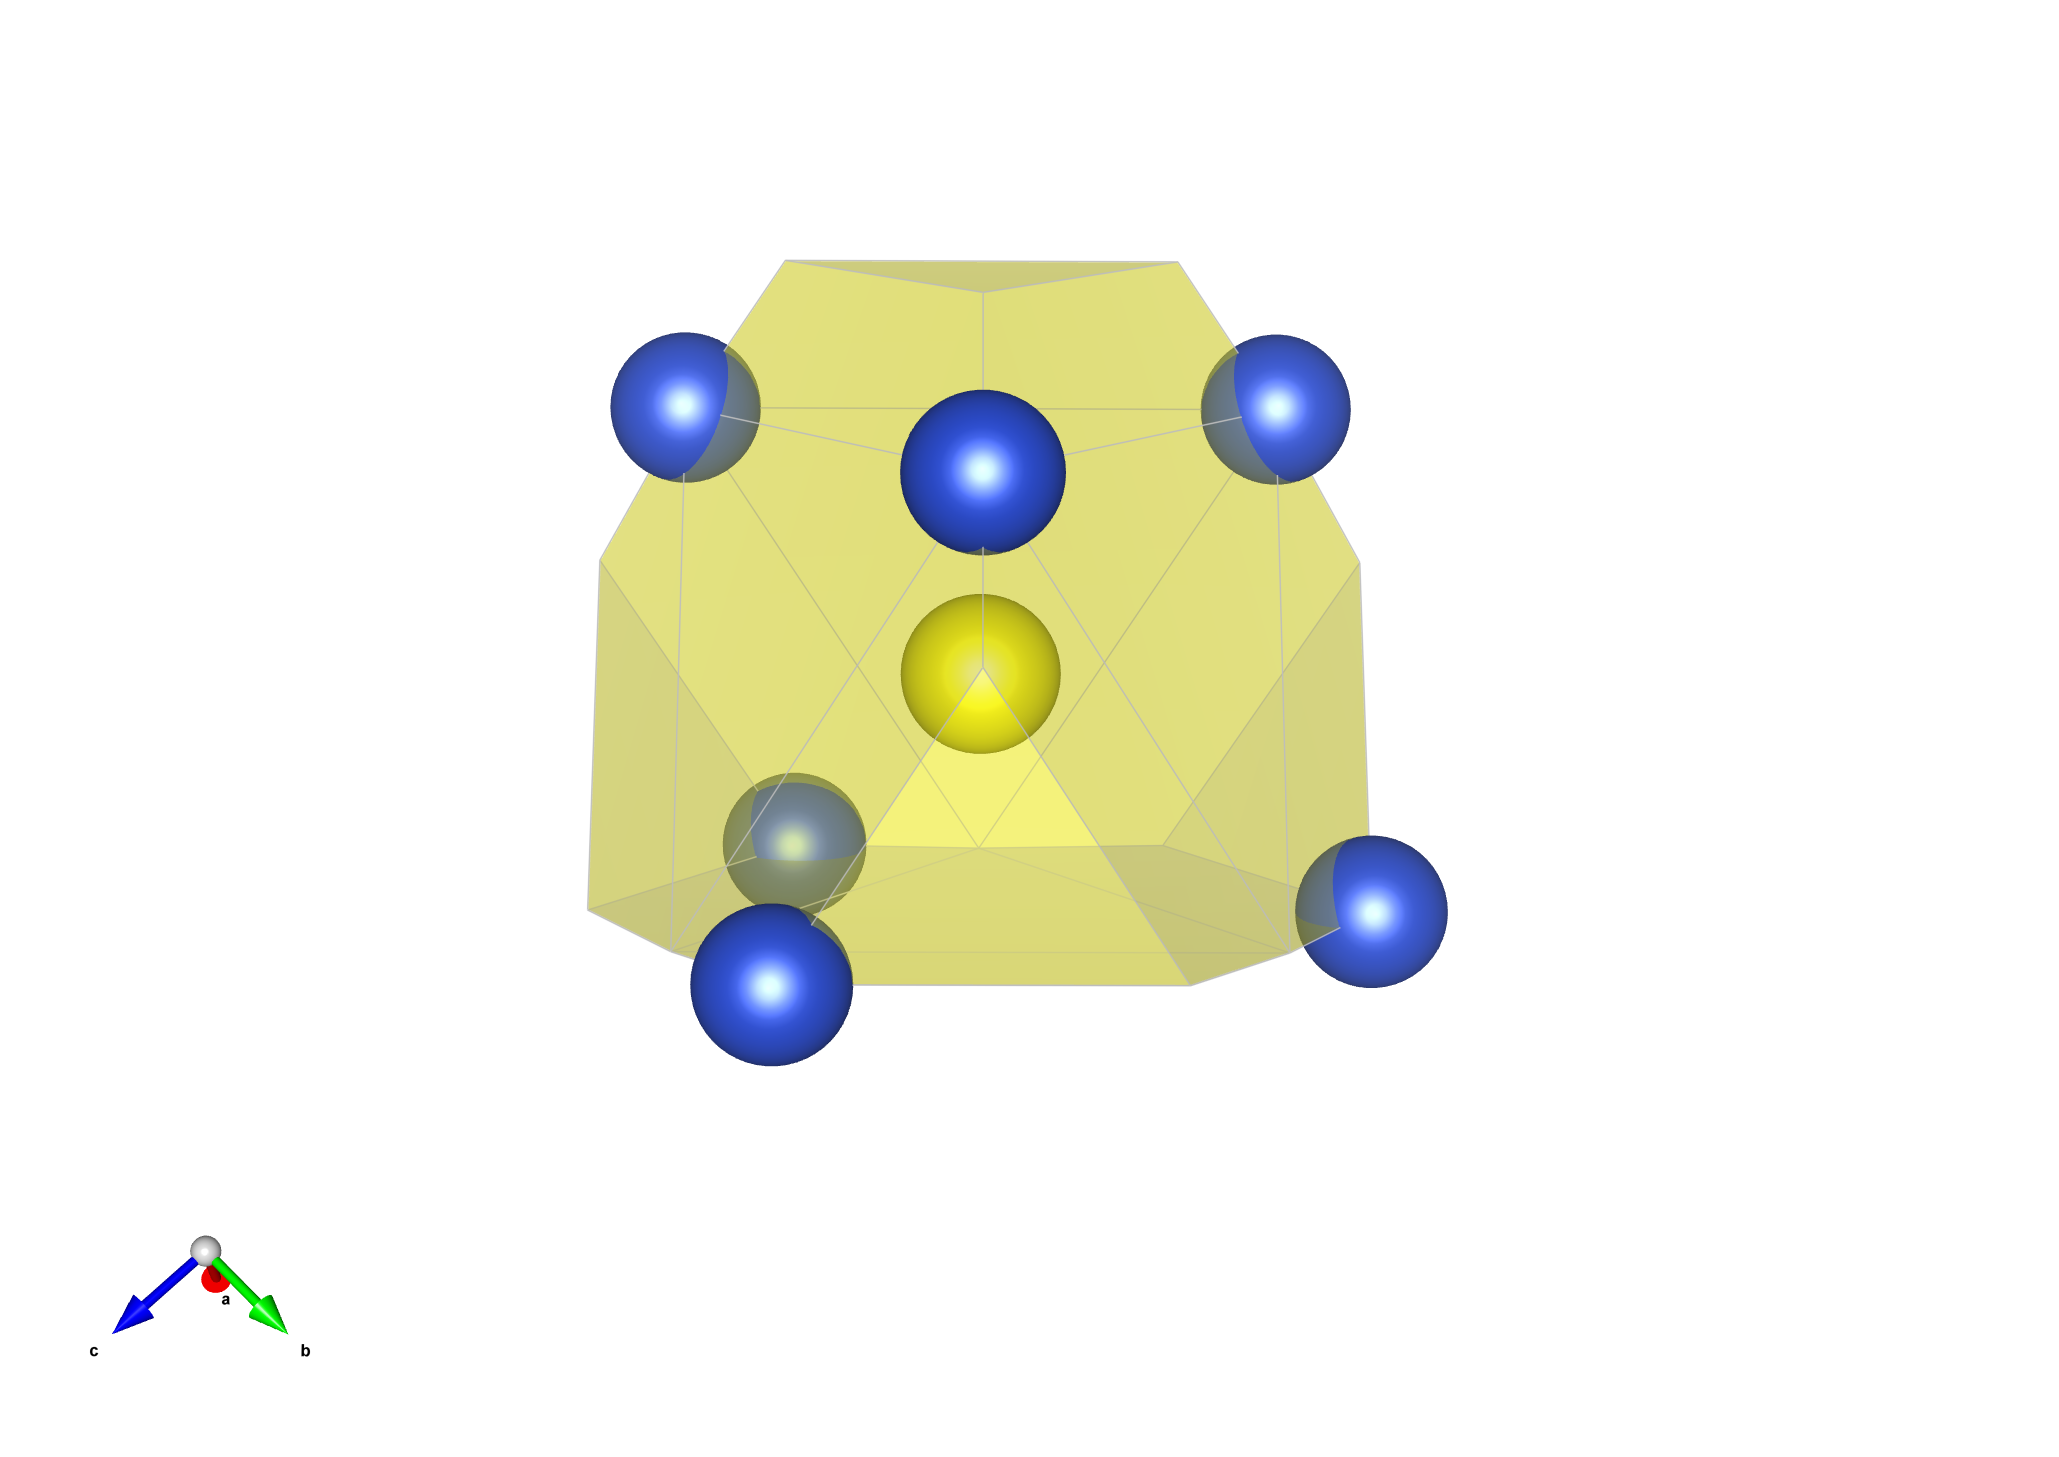
\includegraphics[width=0.9\linewidth]{var_1} \\ б)
  \end{minipage}
\vfill

  \begin{minipage}[ht]{0.45\linewidth}\centering
    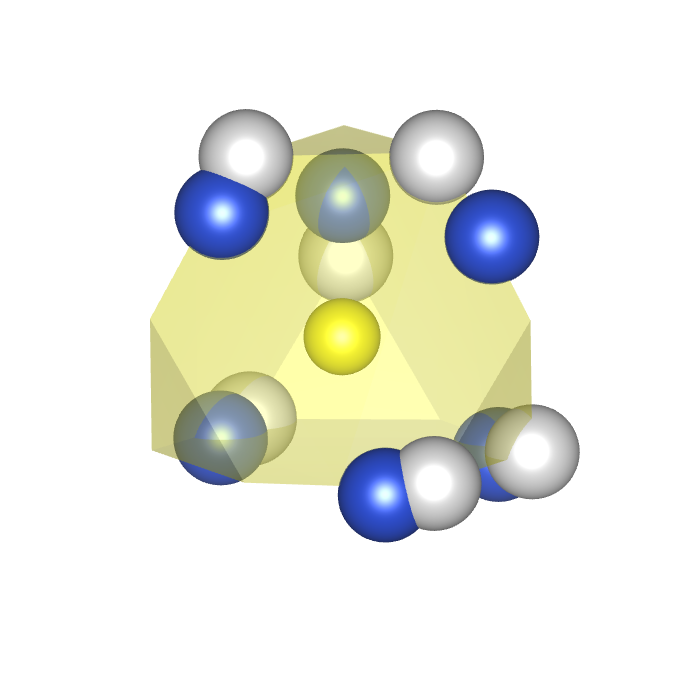
\includegraphics[width=0.9\linewidth]{var_2} \\ в)
  \end{minipage}
						\hfill
 \begin{minipage}[ht]{0.45\linewidth}\centering
    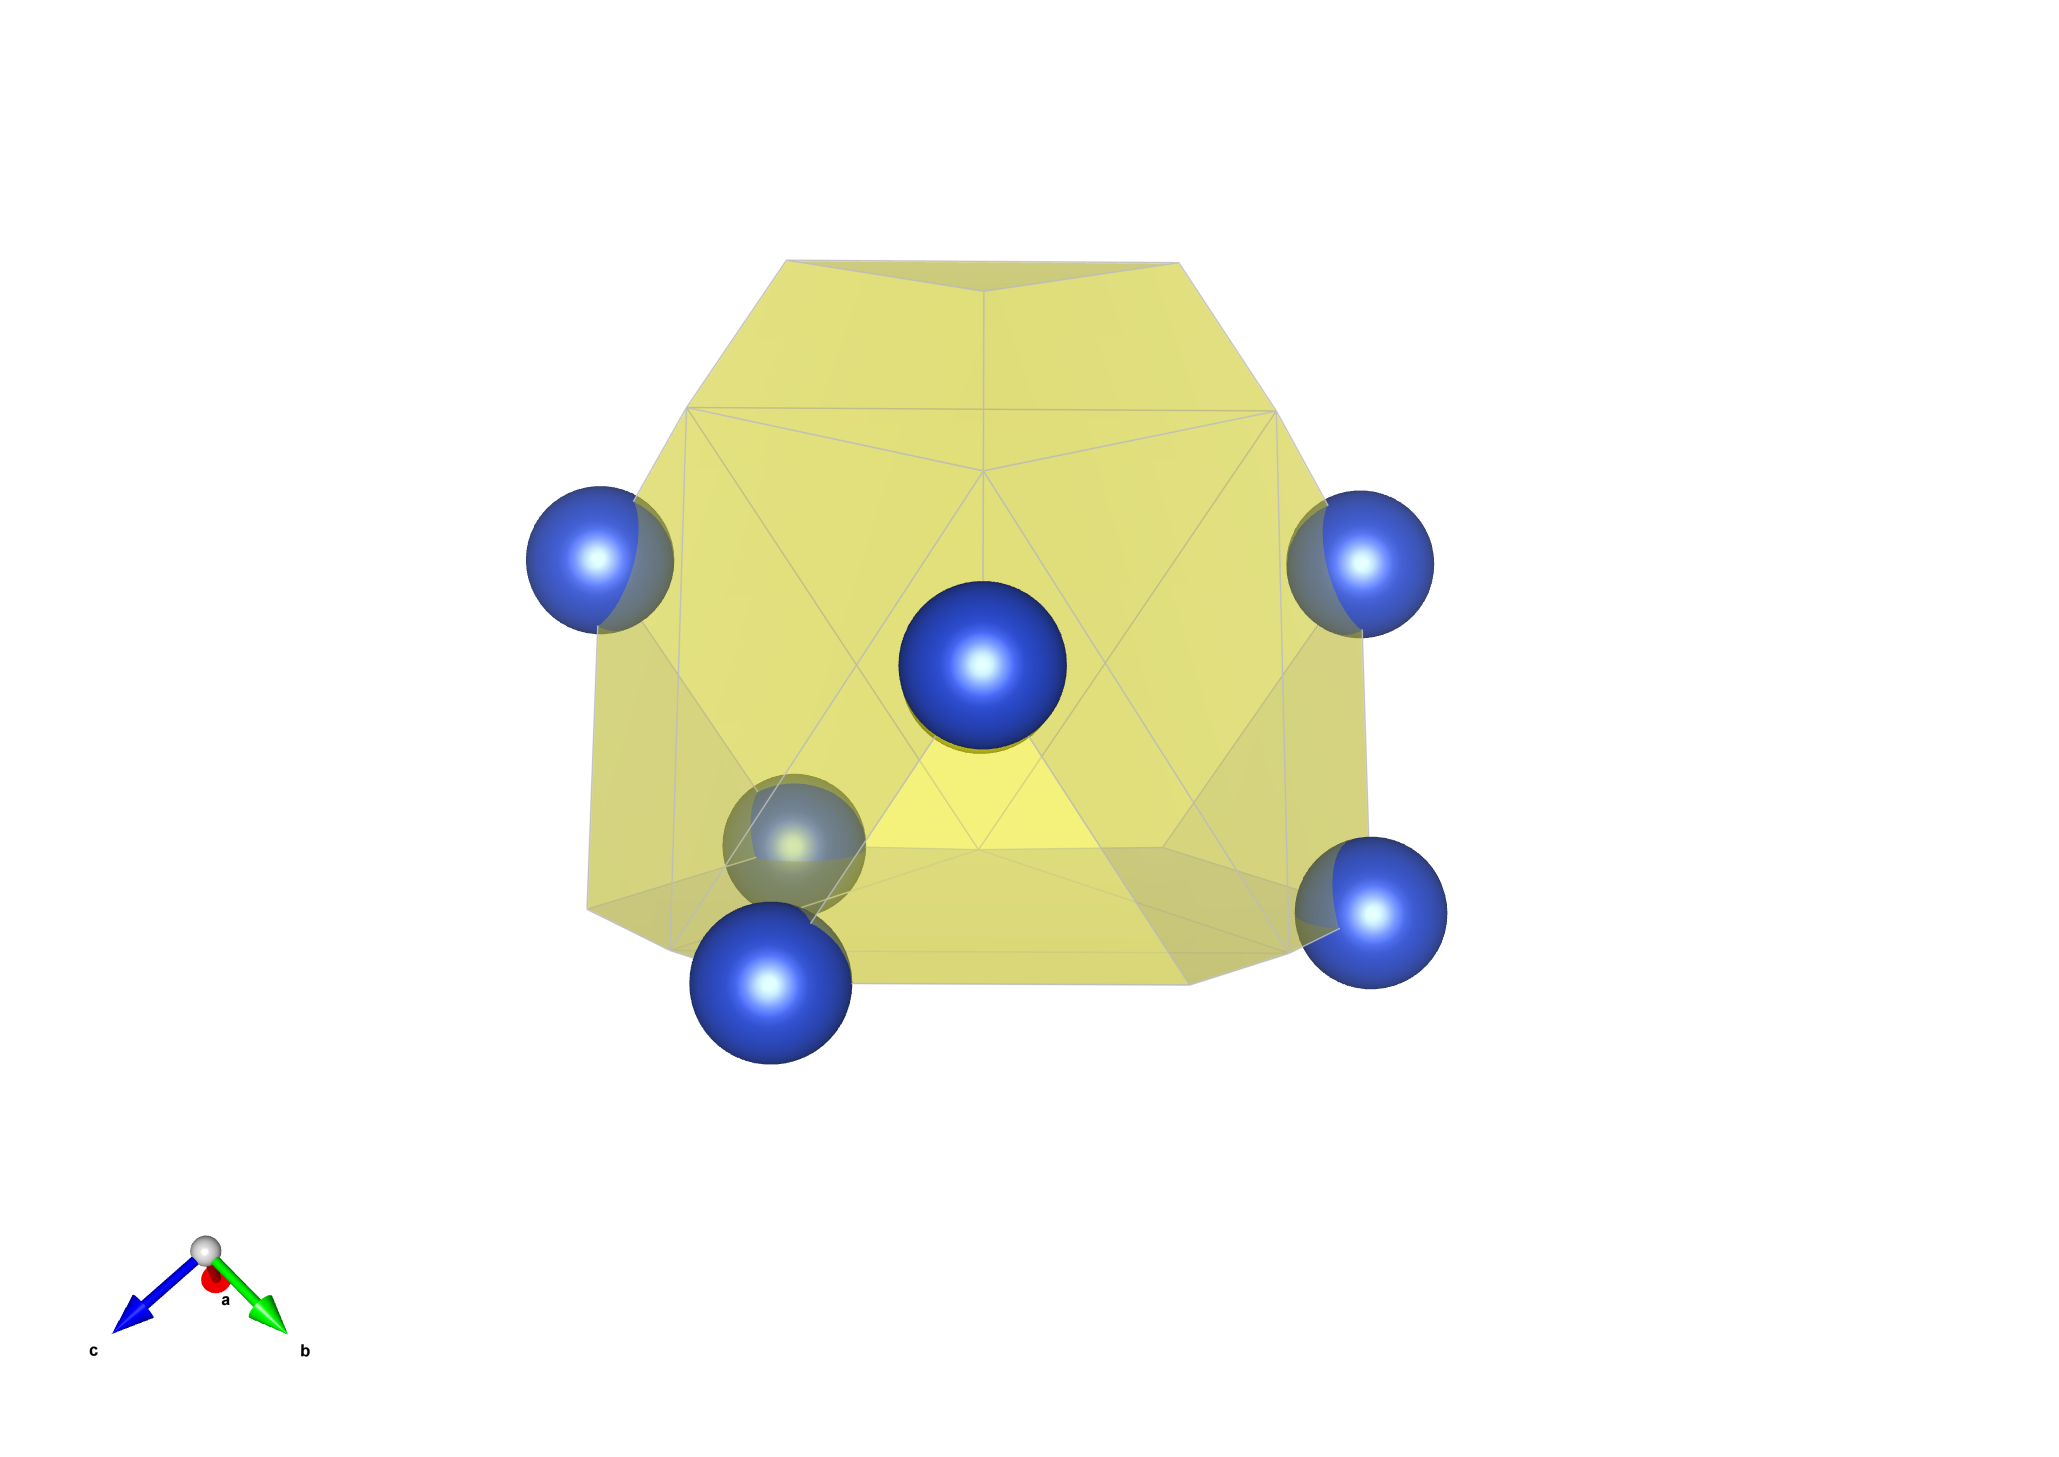
\includegraphics[width=0.9\linewidth]{var_3} \\ г)
  \end{minipage}
\vfill

  \begin{minipage}[ht]{0.45\linewidth}\centering
    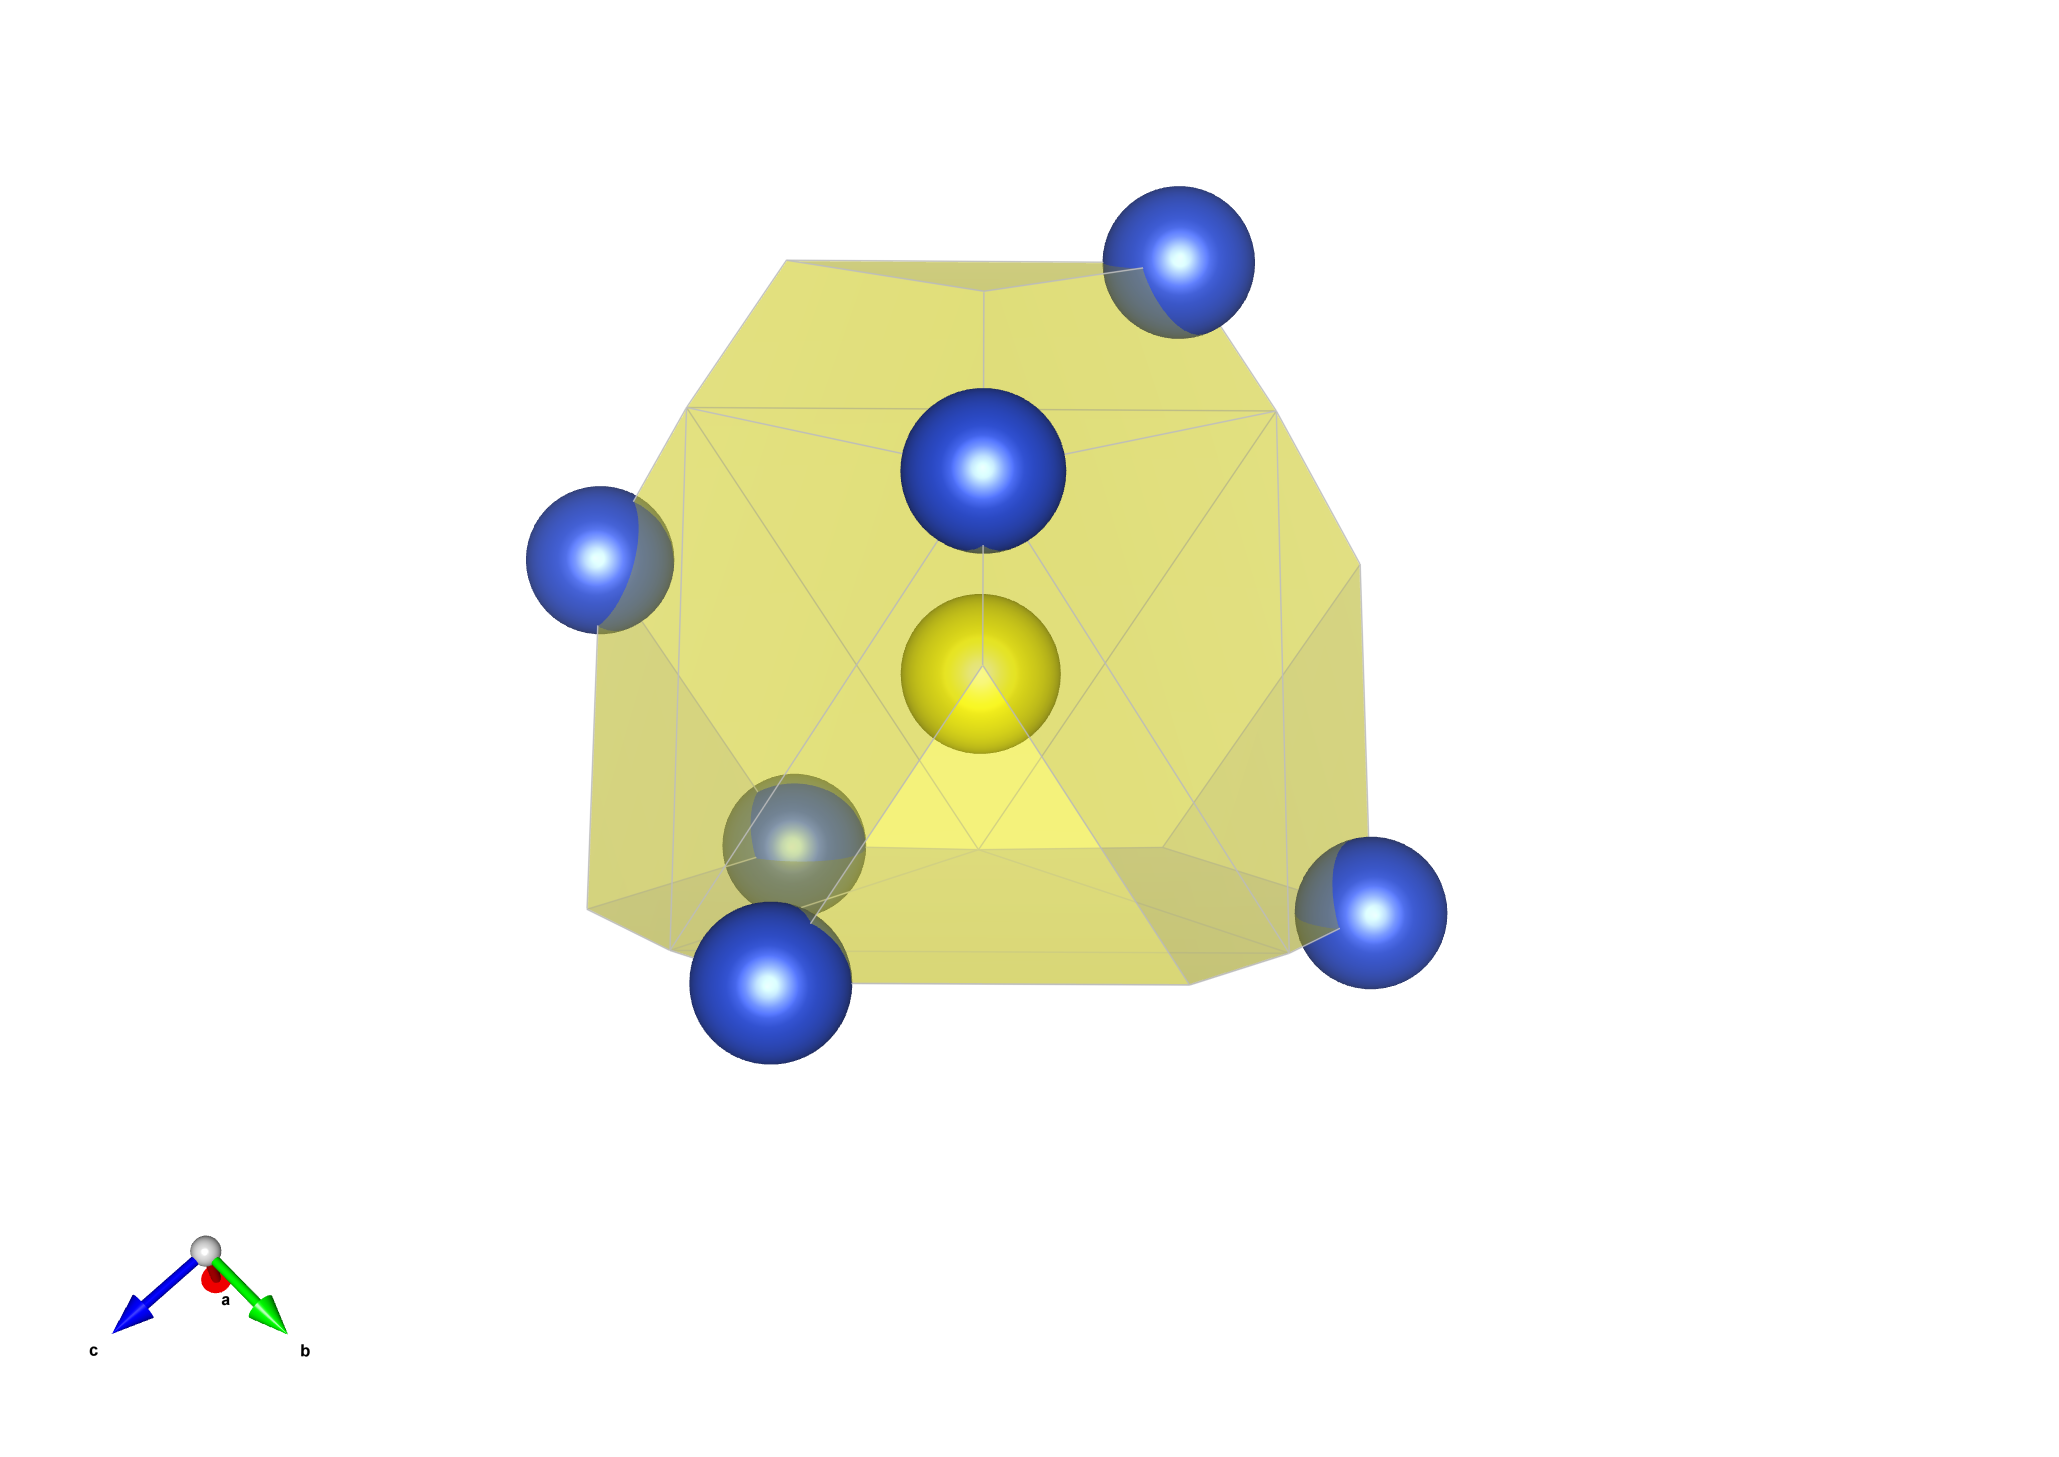
\includegraphics[width=0.9\linewidth]{var_4} \\ д)
  \end{minipage}
						\hfill
 \begin{minipage}[ht]{0.45\linewidth}\centering
    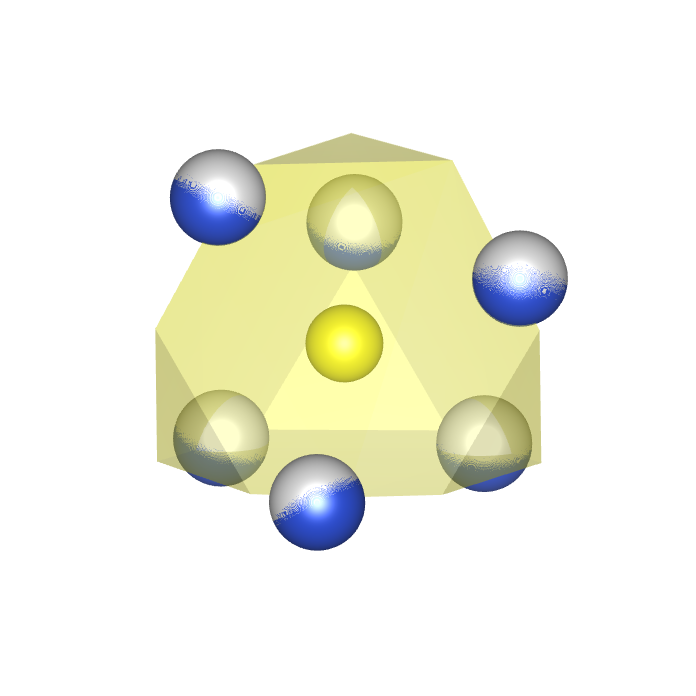
\includegraphics[width=0.9\linewidth]{var_5} \\ е)
  \end{minipage}
      \caption[Изображения лавесовских полиэдров синтетического теннантита Cu\textsubscript{12}As\textsubscript{4}S\textsubscript{13}, для которых рассчитывалась энергия элементарной ячейки. Варианты с 0 по 5 включительно]{Изображения лавесовских полиэдров синтетического теннантита Cu\textsubscript{12}As\textsubscript{4}S\textsubscript{13}, для которых рассчитывалась энергия элементарной ячейки. Варианты с 0 по 5 включительно}
    \label{img:laves1}
\end{figure}

\begin{figure}[p!]
  \begin{minipage}[ht]{0.45\linewidth}\centering
    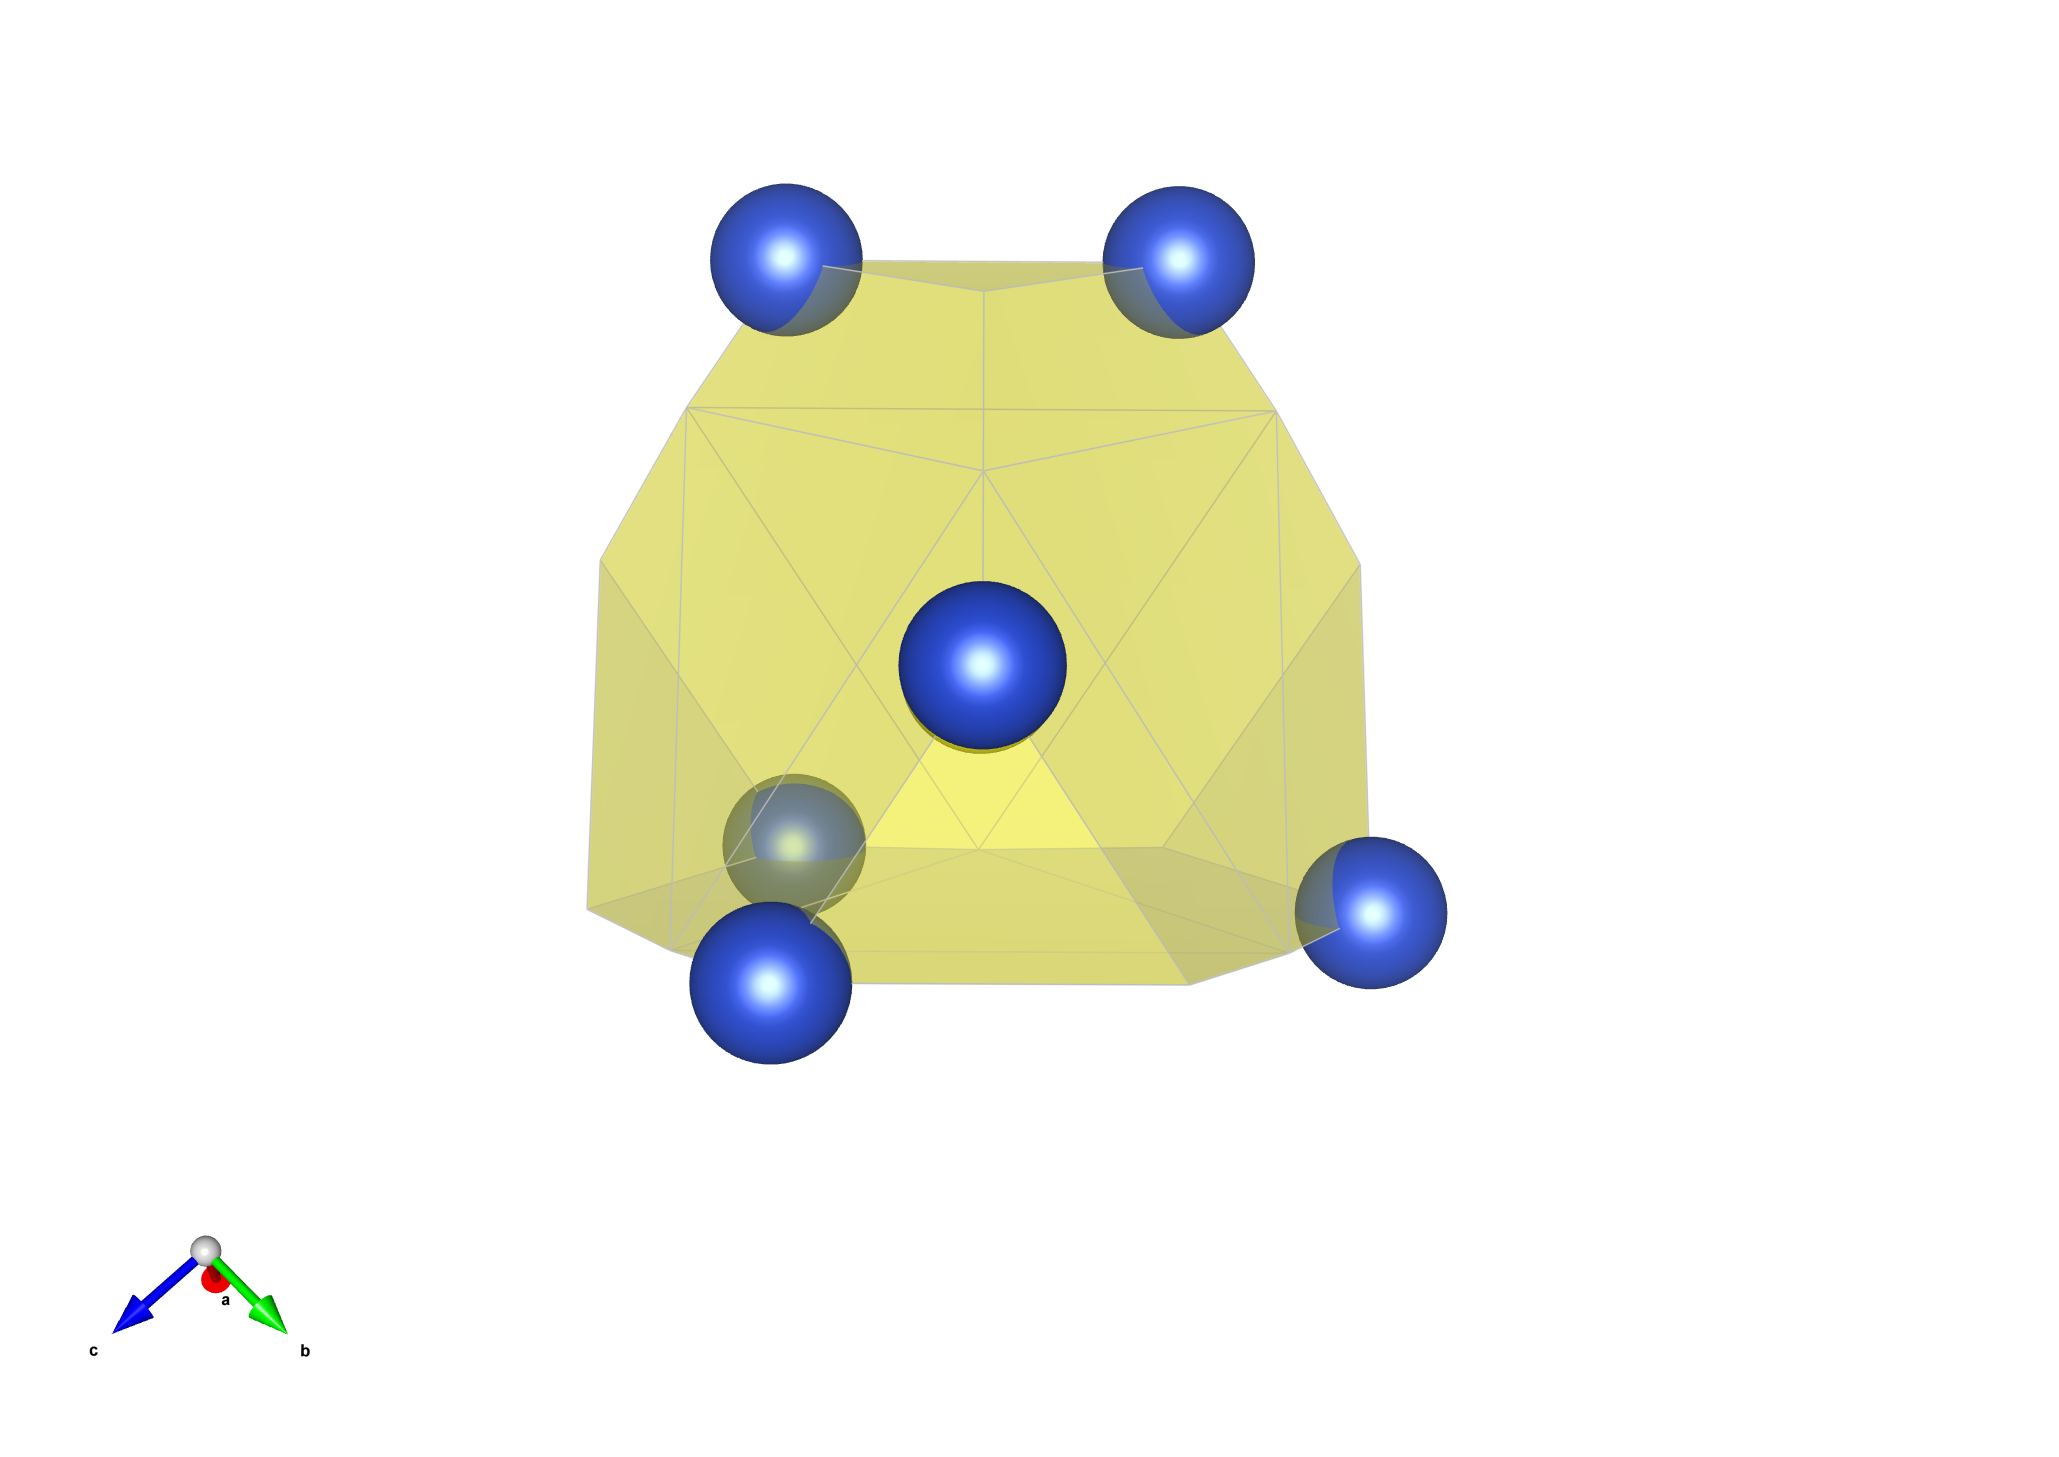
\includegraphics[width=0.9\linewidth]{var_6} \\ а)
  \end{minipage}
						\hfill
 \begin{minipage}[ht]{0.45\linewidth}\centering
    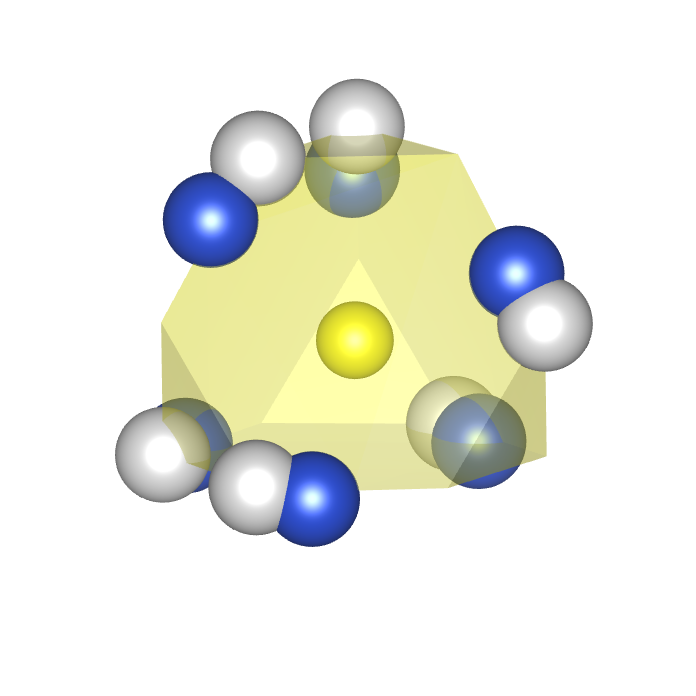
\includegraphics[width=0.9\linewidth]{var_7} \\ б)
  \end{minipage}
\vfill

  \begin{minipage}[ht]{0.45\linewidth}\centering
    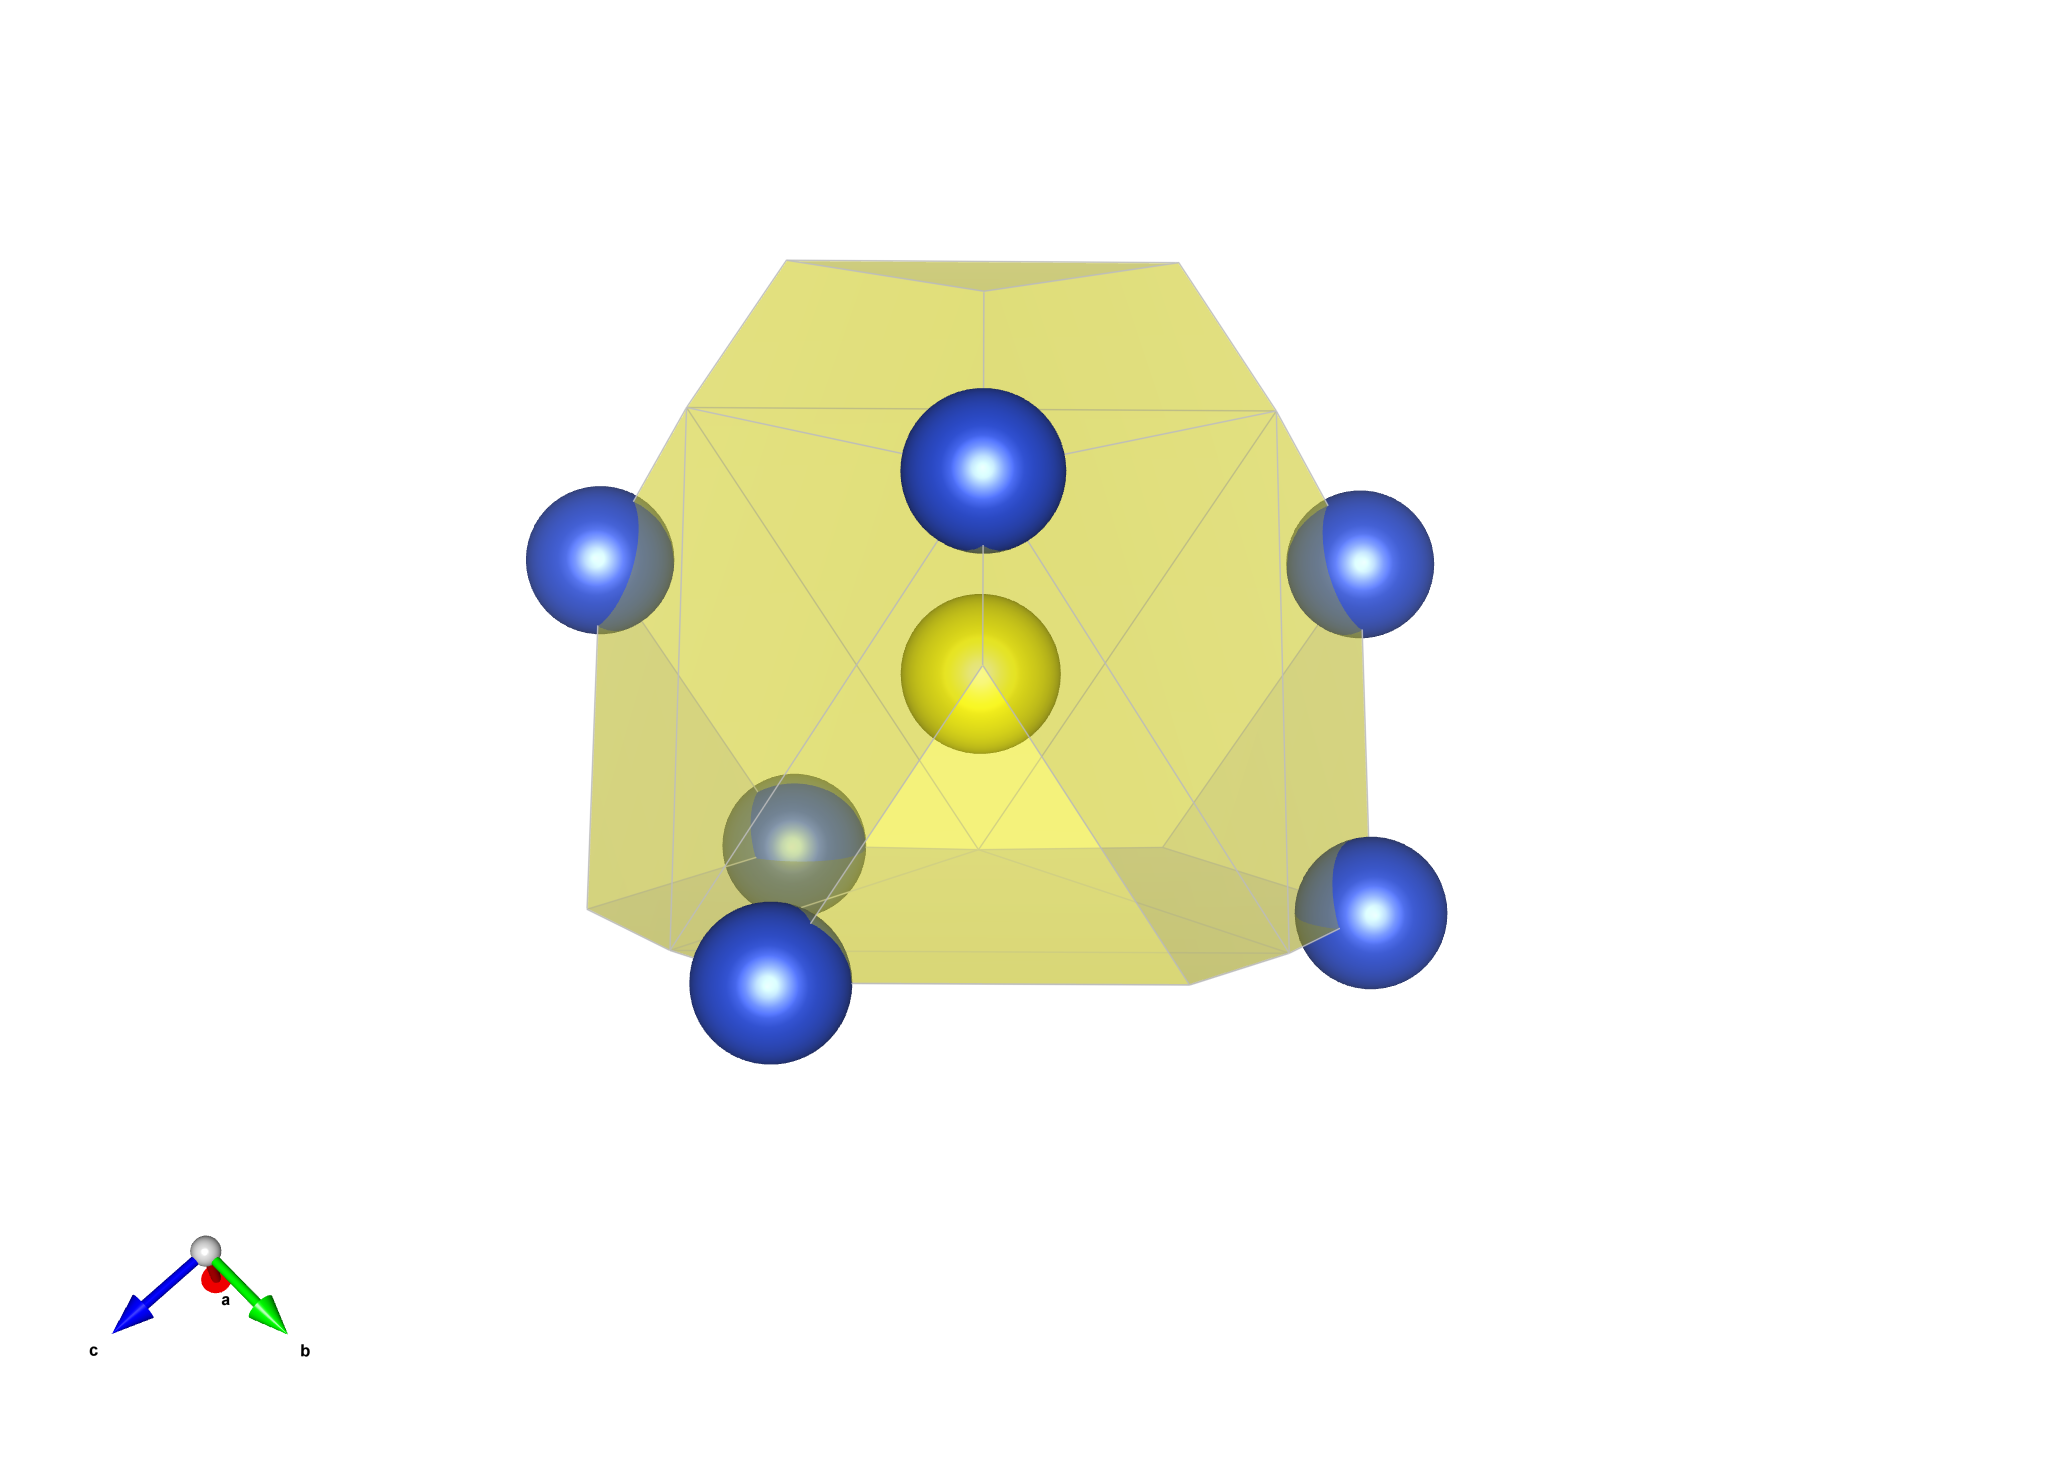
\includegraphics[width=0.9\linewidth]{var_8} \\ в)
  \end{minipage}
						\hfill
 \begin{minipage}[ht]{0.45\linewidth}\centering
    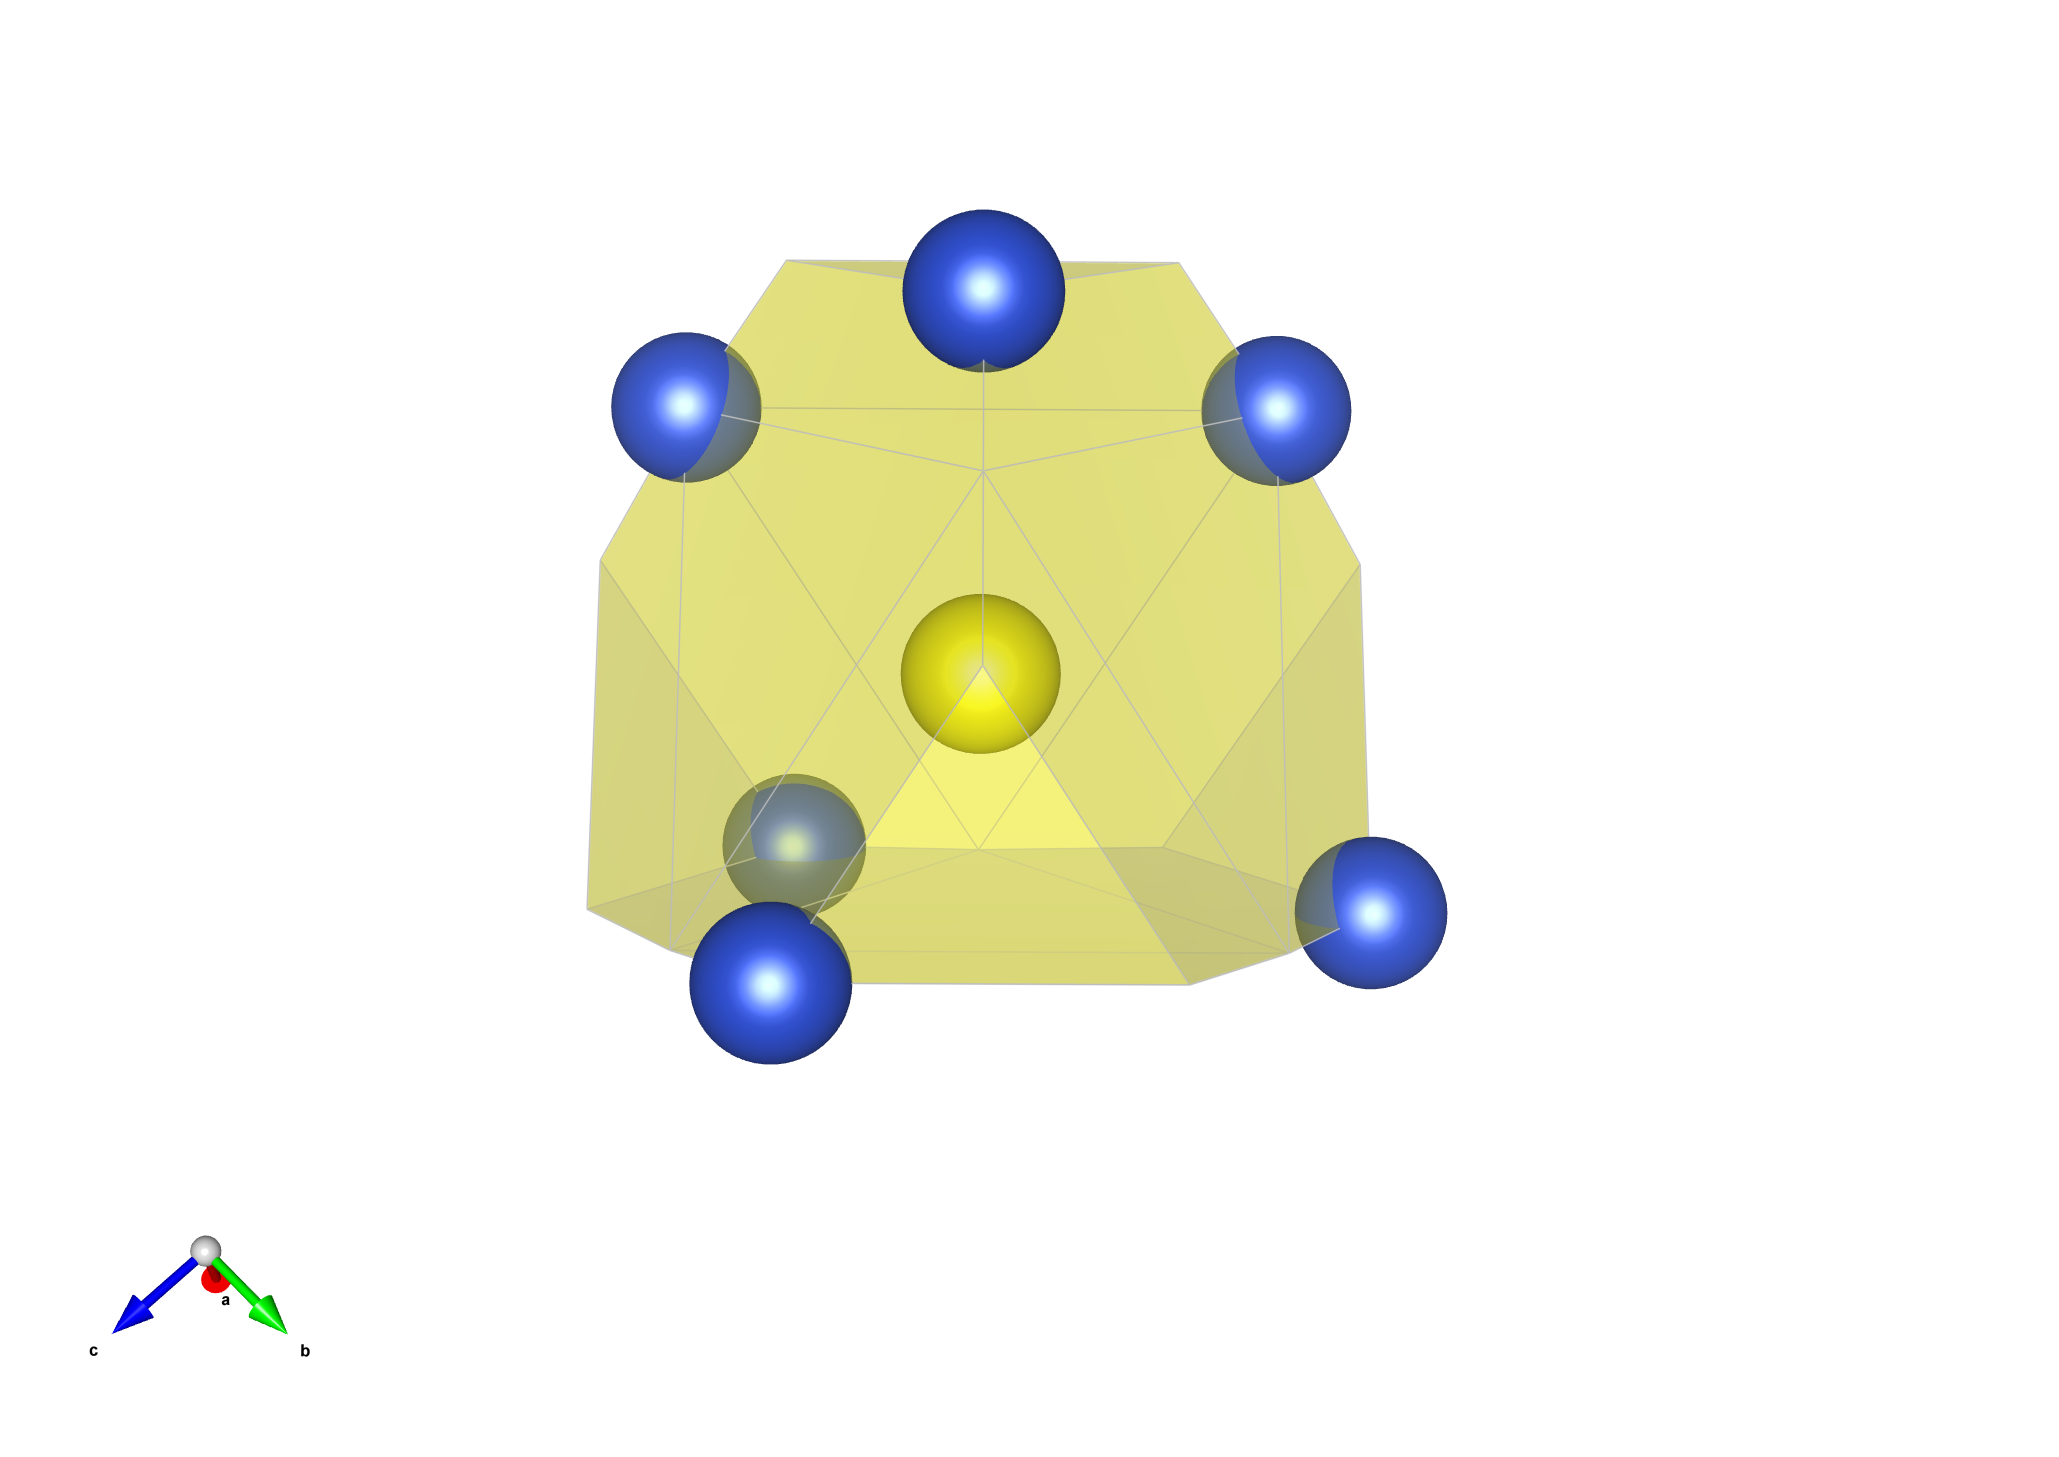
\includegraphics[width=0.9\linewidth]{var_9} \\ г)
  \end{minipage}
\vfill

  \begin{minipage}[ht]{0.45\linewidth}\centering
    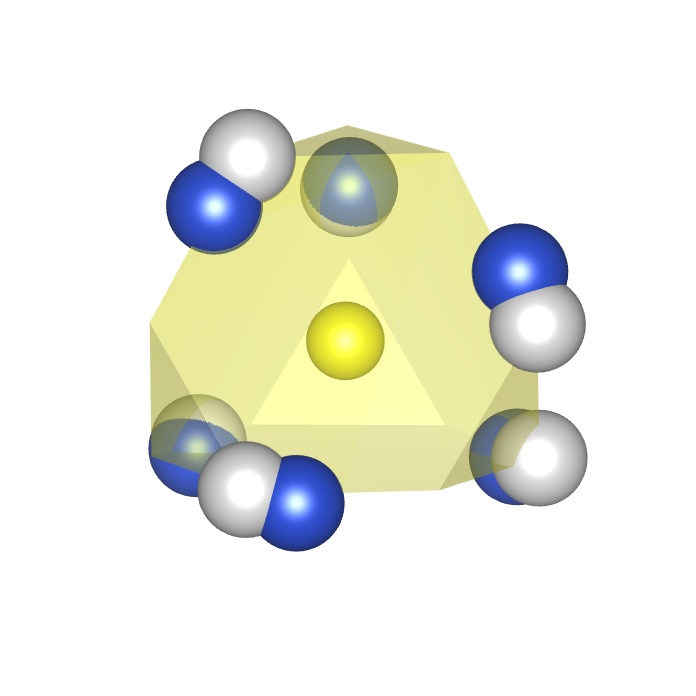
\includegraphics[width=0.9\linewidth]{var_10} \\ д)
  \end{minipage}
						\hfill
 \begin{minipage}[ht]{0.45\linewidth}\centering
    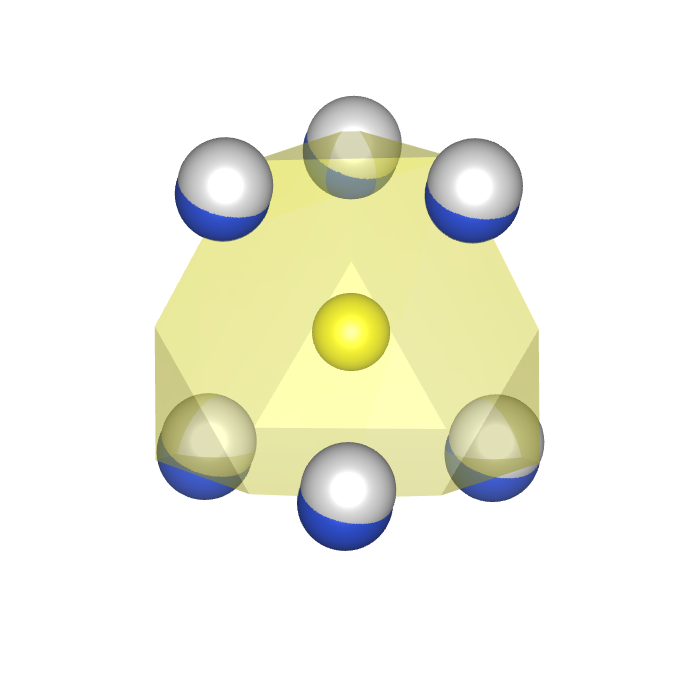
\includegraphics[width=0.9\linewidth]{var_11} \\ е)
  \end{minipage}
      \caption[Изображения лавесовских полиэдров синтетического теннантита Cu\textsubscript{12}As\textsubscript{4}S\textsubscript{13}, для которых рассчитывалась энергия элементарной ячейки. Варианты с 6 по 11 включительно]{Изображения лавесовских полиэдров синтетического теннантита Cu\textsubscript{12}As\textsubscript{4}S\textsubscript{13}, для которых рассчитывалась энергия элементарной ячейки. Варианты с 6 по 11 включительно}
    \label{img:laves2}
\end{figure}



\begin{figure}[p!]
  \begin{minipage}[ht]{0.45\linewidth}\centering
    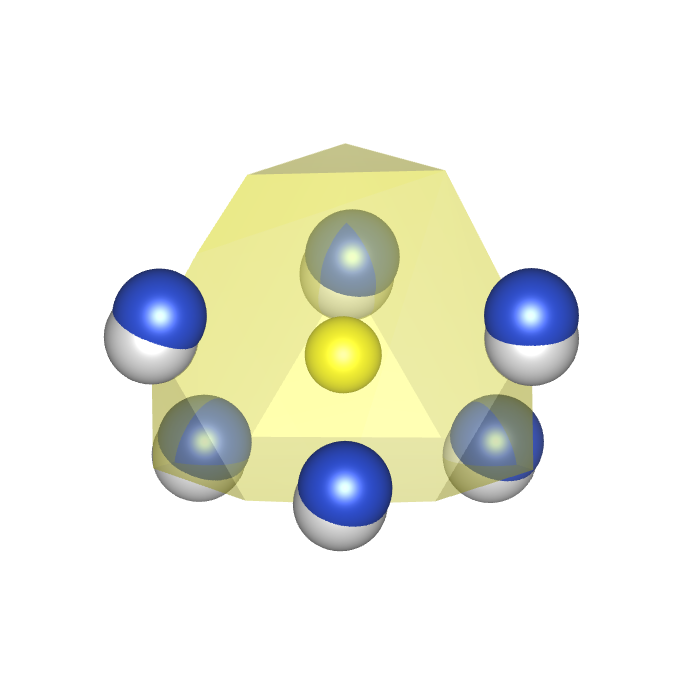
\includegraphics[width=0.9\linewidth]{var_12} \\ а)
  \end{minipage}
\hfill
 \begin{minipage}[ht]{0.45\linewidth}\centering
    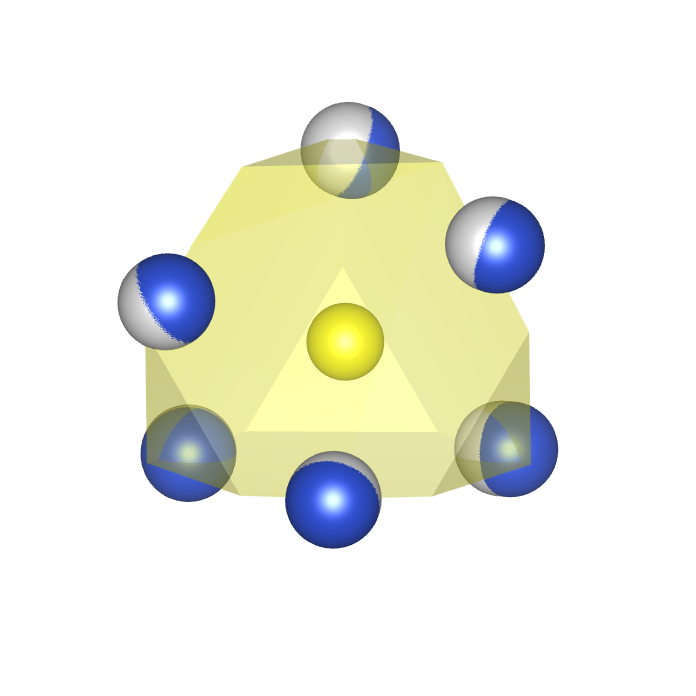
\includegraphics[width=0.9\linewidth]{var_13} \\ б)
  \end{minipage}
\vfill
  \begin{minipage}[ht]{0.45\linewidth}\centering
    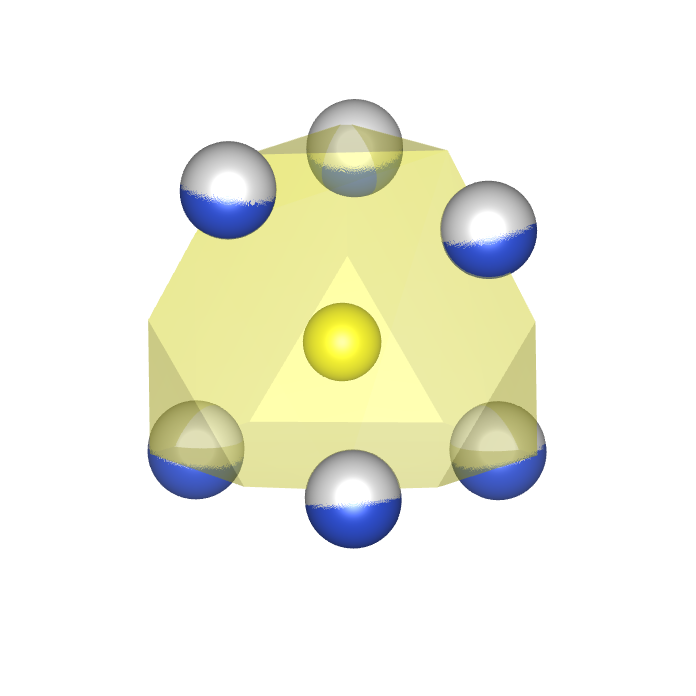
\includegraphics[width=0.9\linewidth]{var_14} \\ в)
  \end{minipage}
	\hfill
 \begin{minipage}[ht]{0.45\linewidth}\centering
    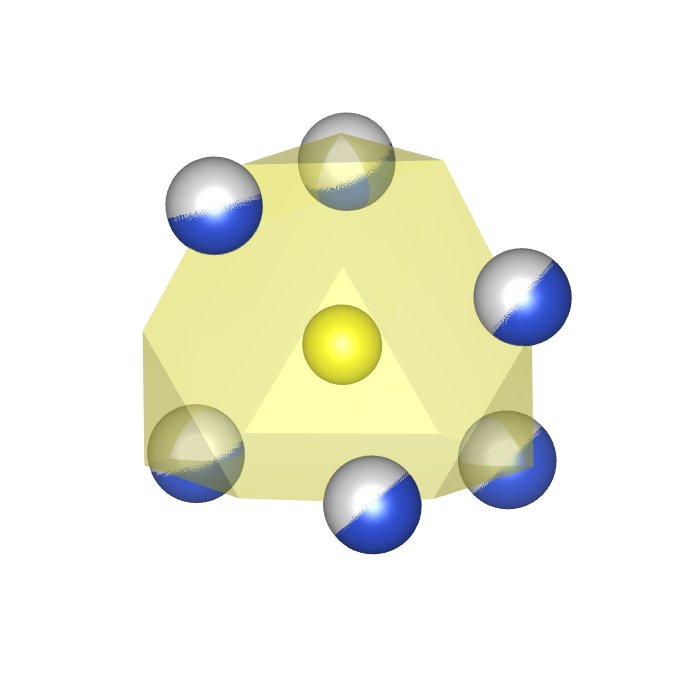
\includegraphics[width=0.9\linewidth]{var_15} \\ г)
  \end{minipage}
\vfill

  \begin{minipage}[ht]{0.45\linewidth}\centering

  \end{minipage}
						\hfill
 \begin{minipage}[ht]{0.45\linewidth}\centering

  \end{minipage}
      \caption[Изображения лавесовских полиэдров синтетического теннантита Cu\textsubscript{12}As\textsubscript{4}S\textsubscript{13}, для которых рассчитывалась энергия элементарной ячейки. Варианты с 12 по 15 включительно]{Изображения лавесовских полиэдров синтетического теннантита Cu\textsubscript{12}As\textsubscript{4}S\textsubscript{13}, для которых рассчитывалась энергия элементарной ячейки. Варианты с 6 по 11 включительно}
    \label{img:laves3}
\end{figure}


\begin{figure}[p!]
  \begin{minipage}[ht]{0.45\linewidth}\centering
    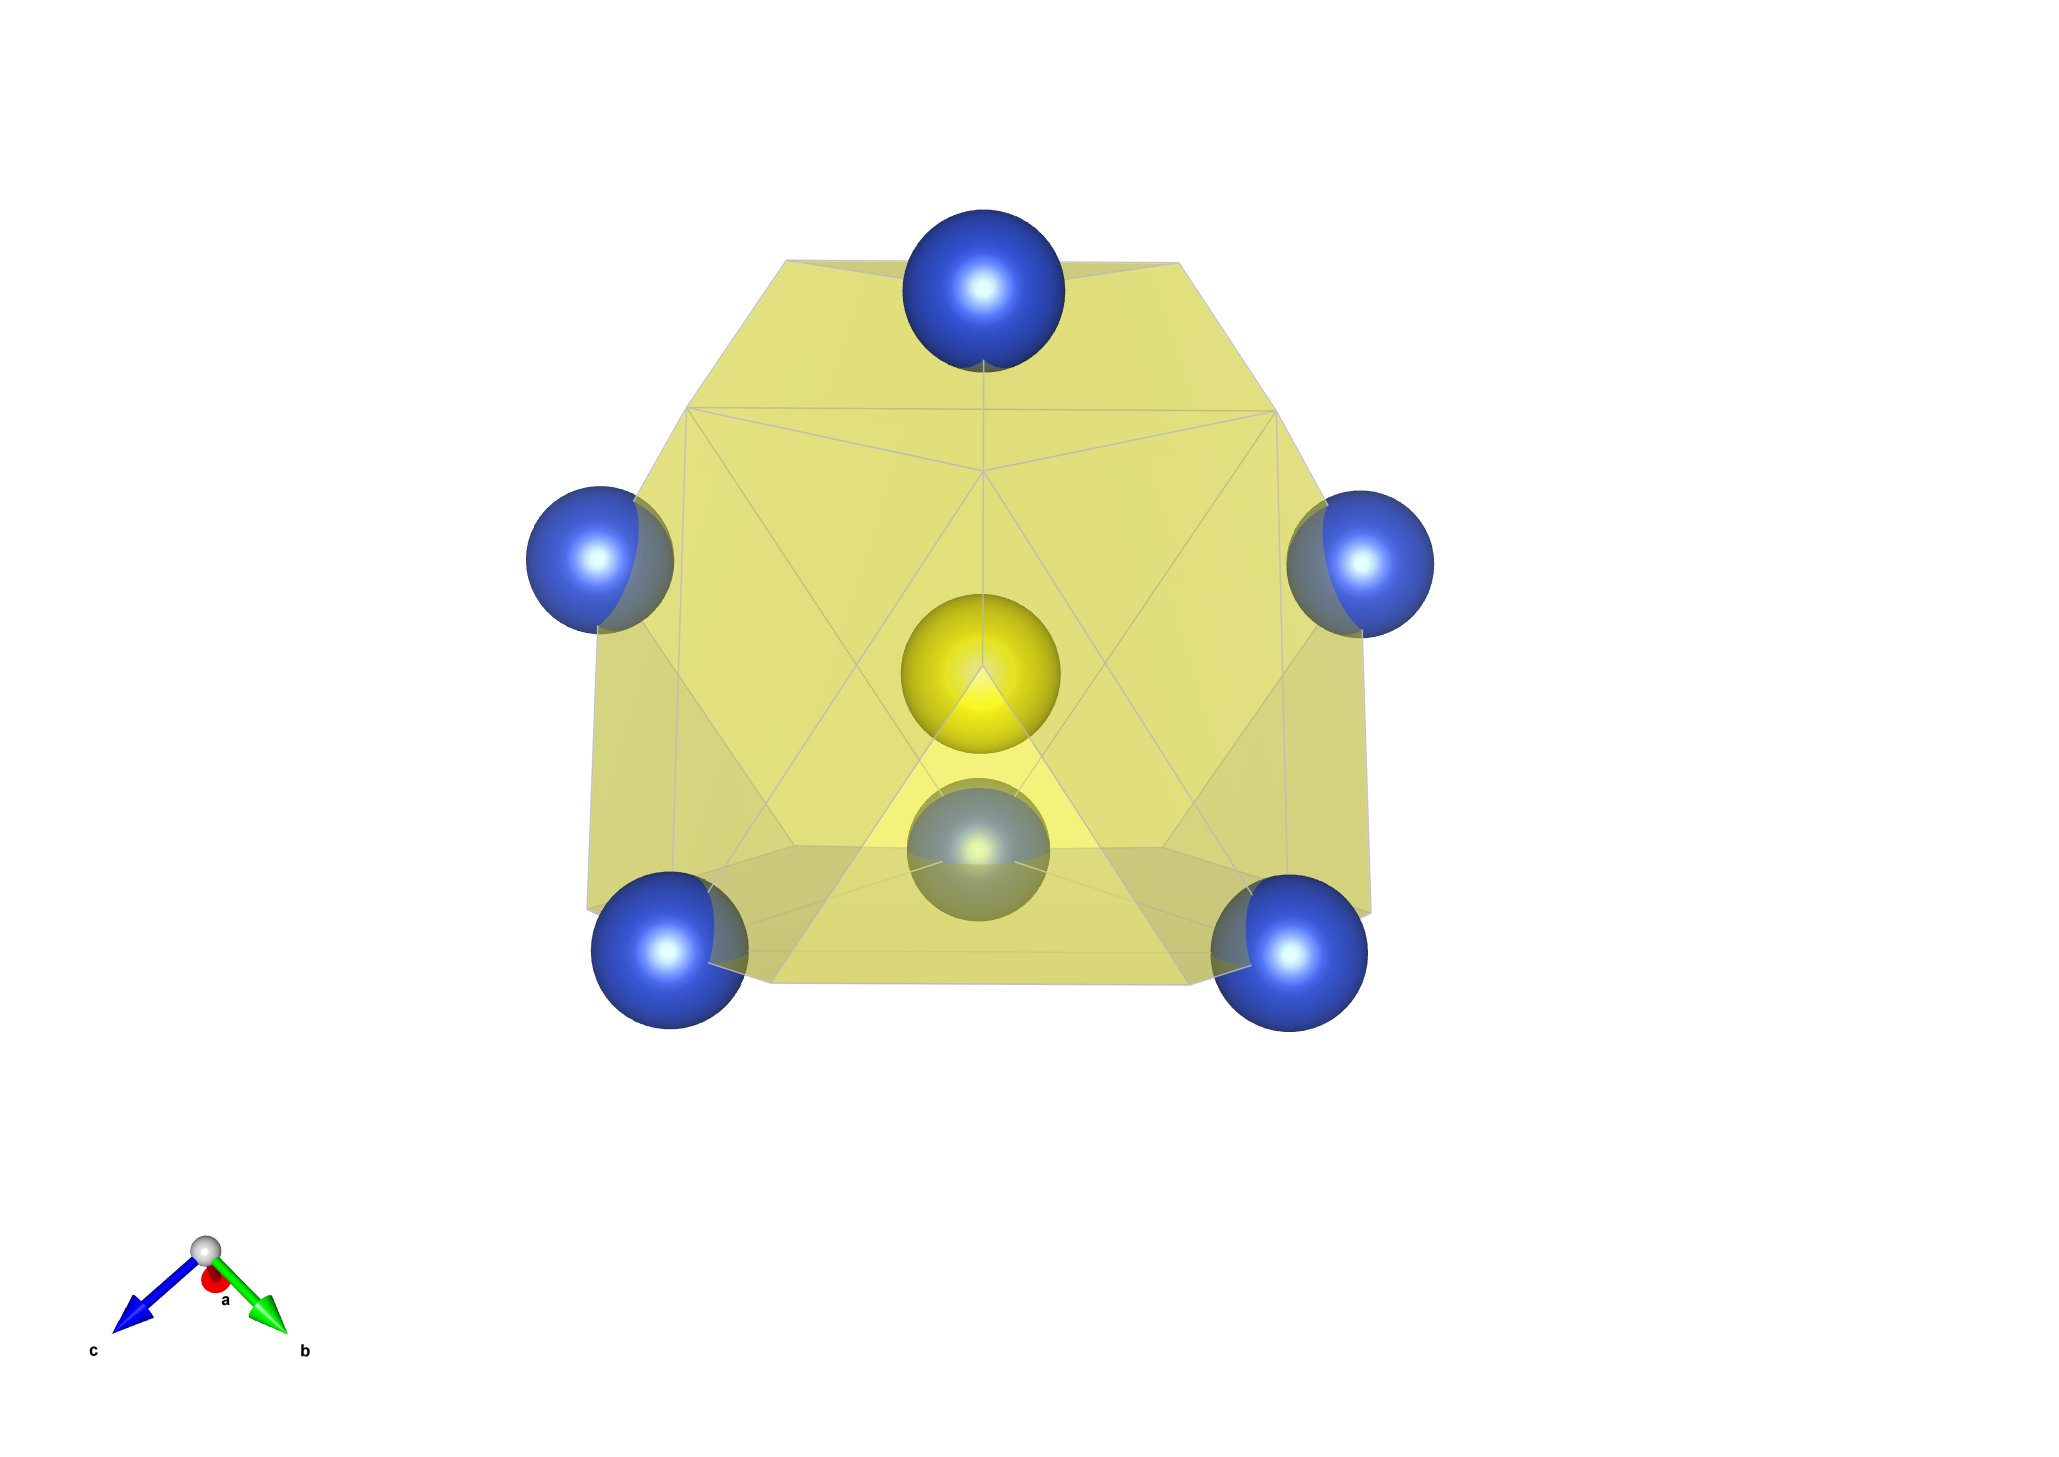
\includegraphics[width=0.9\linewidth]{var_16} \\ а)
  \end{minipage}
						\hfill
 \begin{minipage}[ht]{0.45\linewidth}\centering
    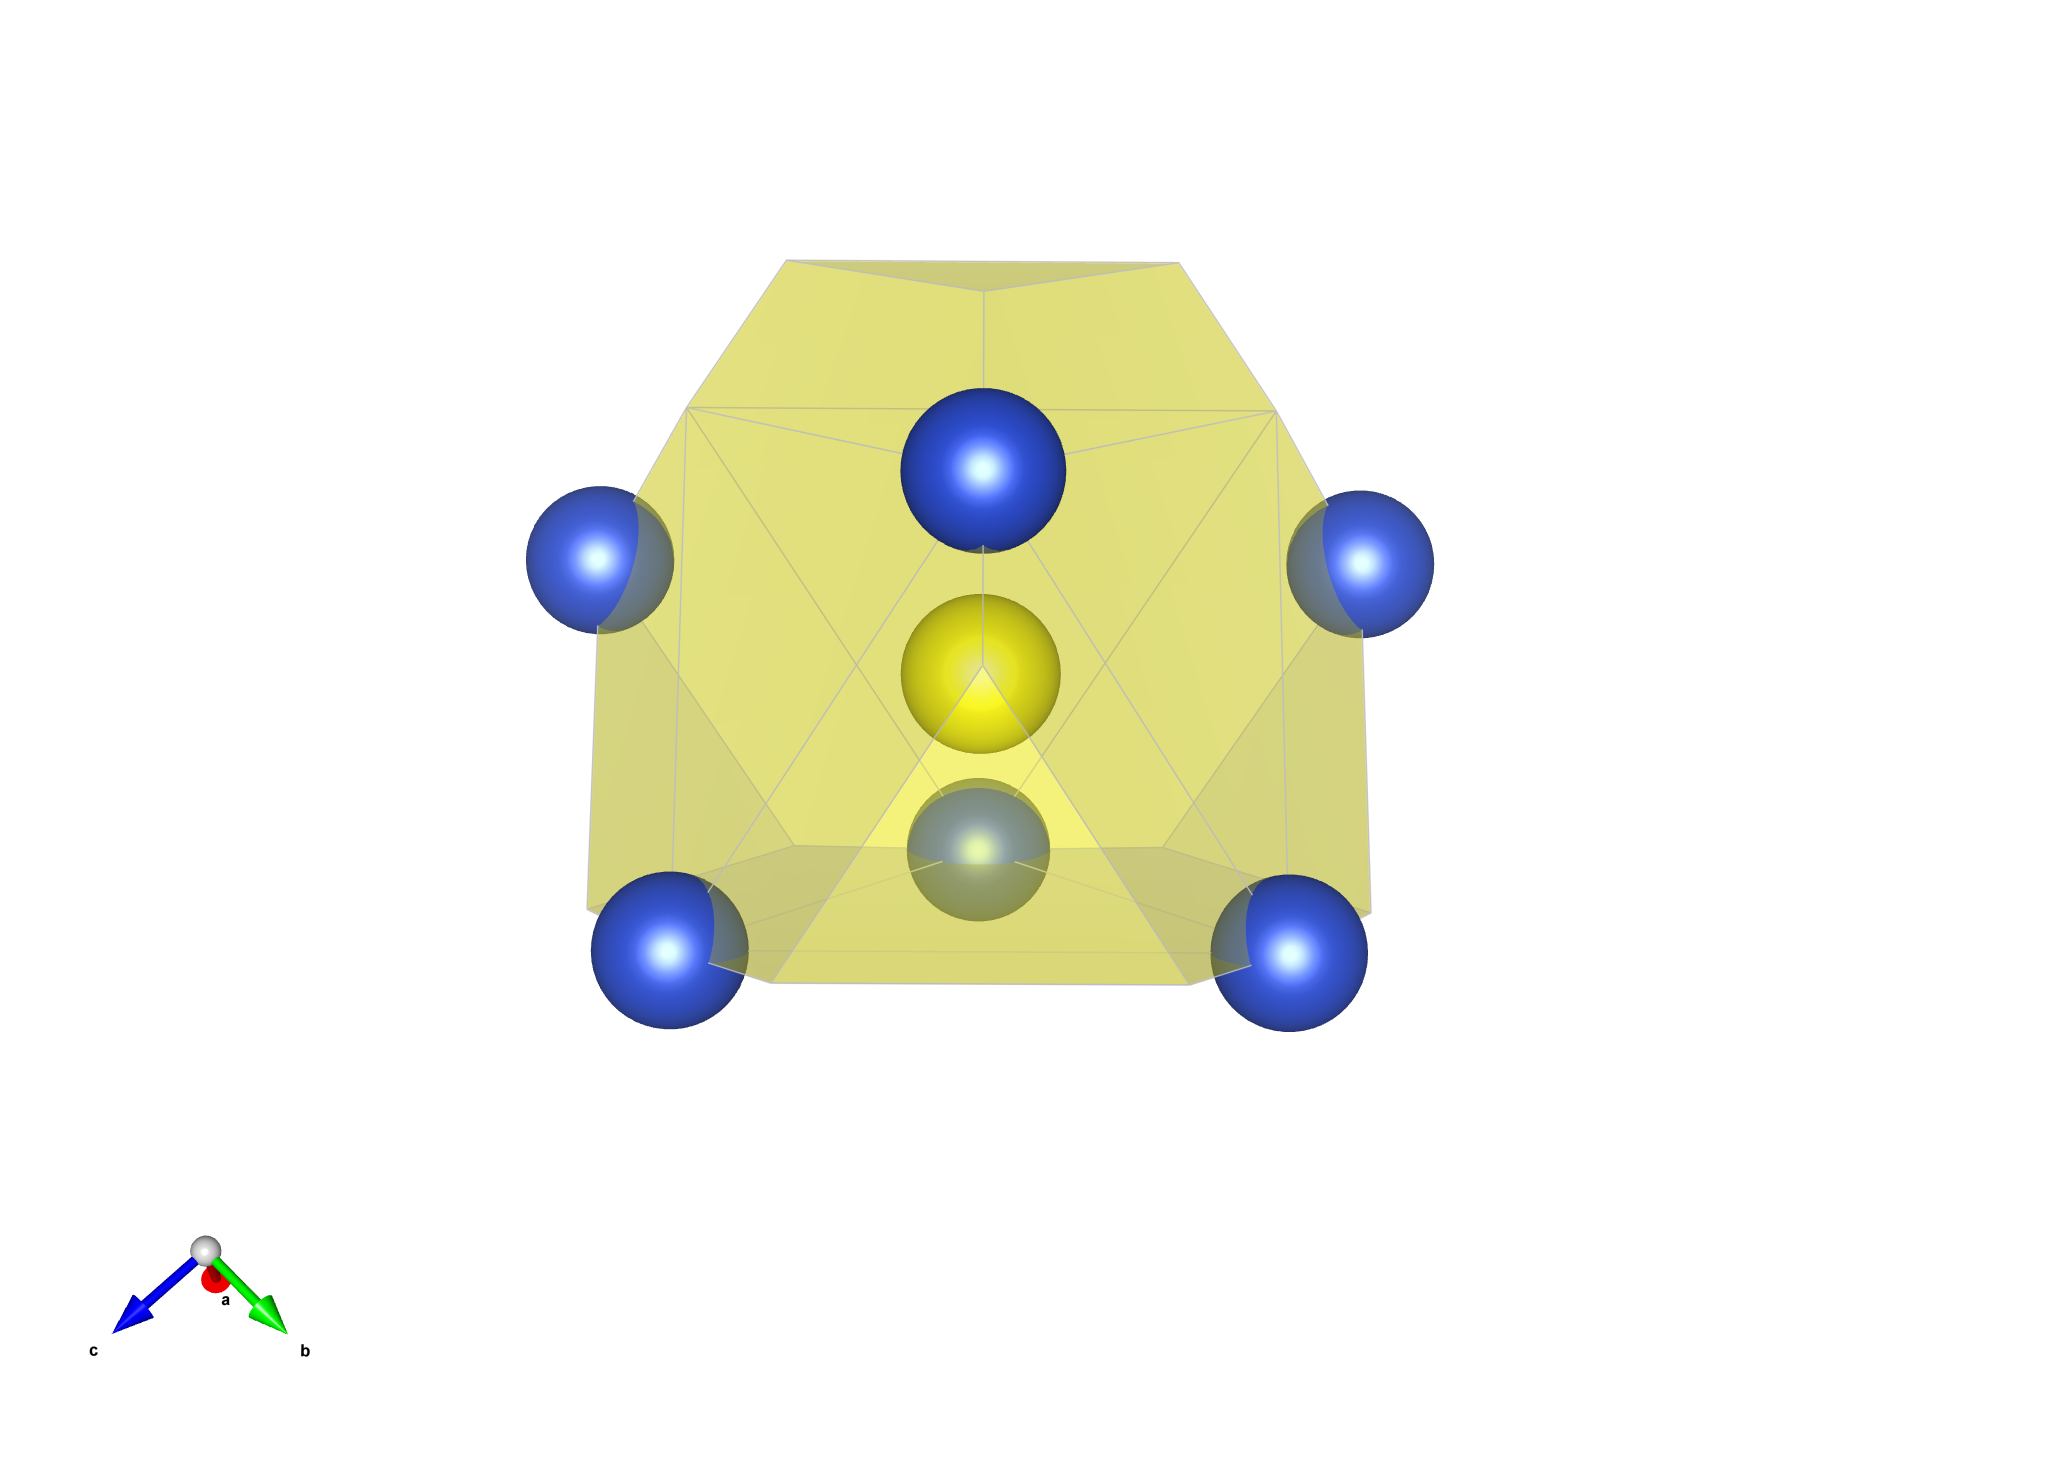
\includegraphics[width=0.9\linewidth]{var_17} \\ б)
  \end{minipage}
\vfill

  \begin{minipage}[ht]{0.45\linewidth}\centering
    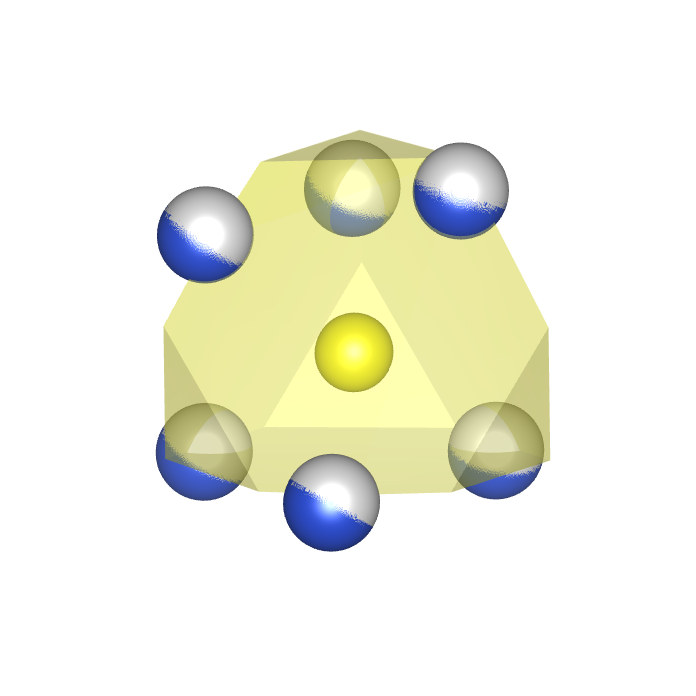
\includegraphics[width=0.9\linewidth]{var_18} \\ в)
  \end{minipage}
						\hfill
 \begin{minipage}[ht]{0.45\linewidth}\centering
    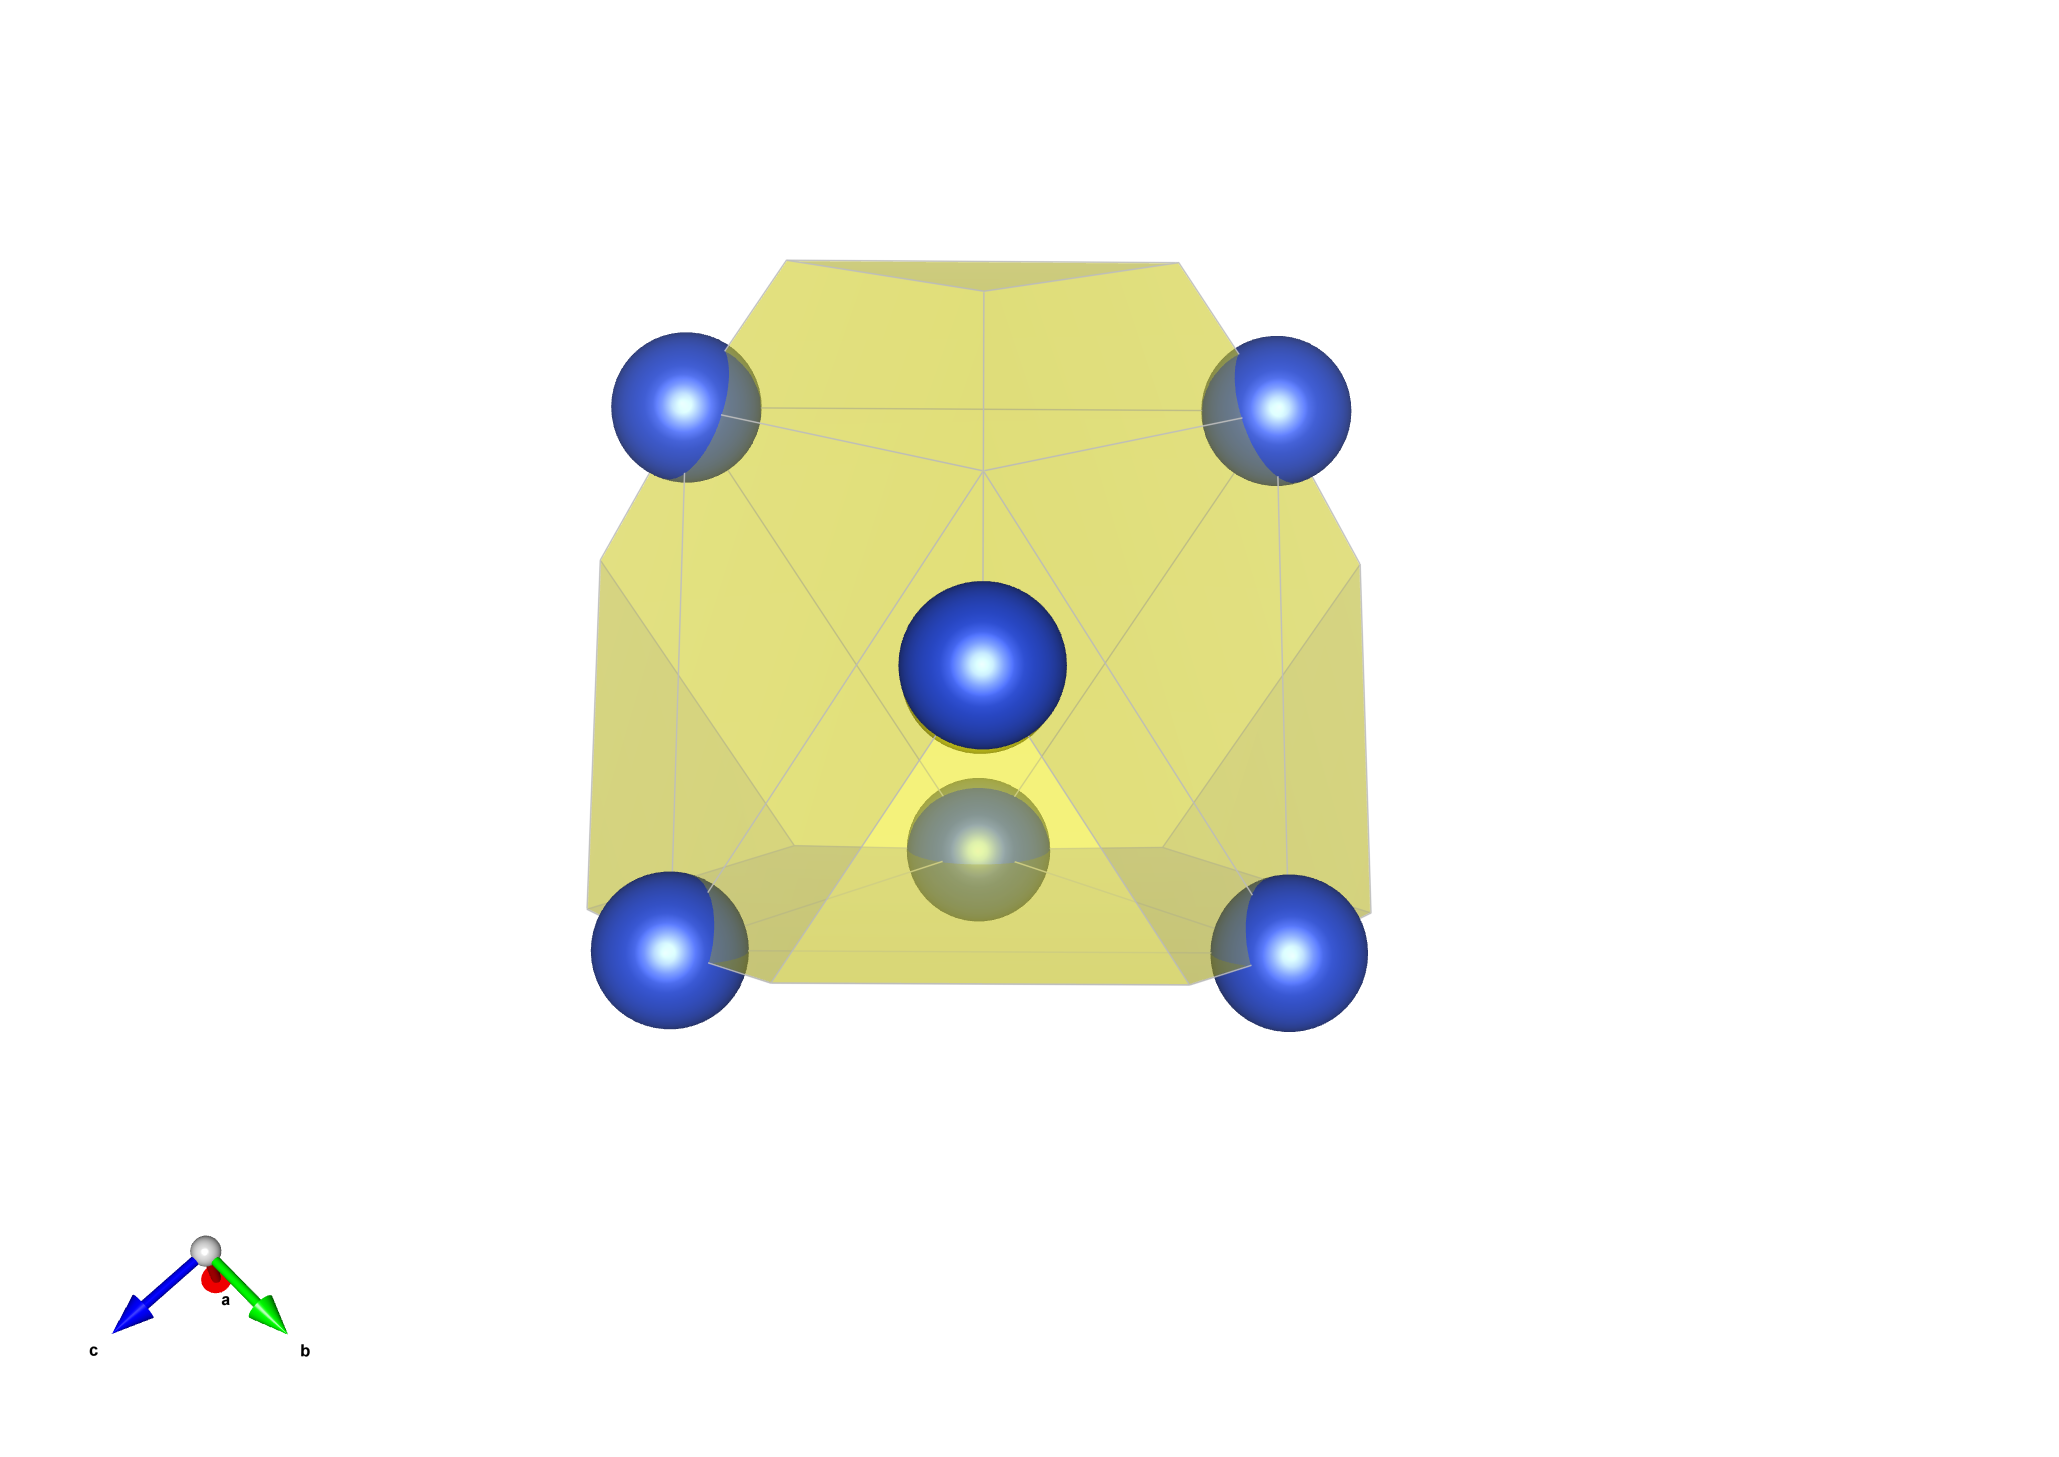
\includegraphics[width=0.9\linewidth]{var_19} \\ г)
  \end{minipage}
\vfill

  \begin{minipage}[ht]{0.45\linewidth}\centering

  \end{minipage}
						\hfill
 \begin{minipage}[ht]{0.45\linewidth}\centering

  \end{minipage}
      \caption[Изображения лавесовских полиэдров синтетического теннантита Cu\textsubscript{12}As\textsubscript{4}S\textsubscript{13}, для которых рассчитывалась энергия элементарной ячейки. Варианты с 16 по 19 включительно]{Изображения лавесовских полиэдров синтетического теннантита Cu\textsubscript{12}As\textsubscript{4}S\textsubscript{13}, для которых рассчитывалась энергия элементарной ячейки. Варианты с 16 по 19 включительно}
    \label{img:laves4}
\end{figure}



\newpage

\clearpage
